\documentclass[12pt]{amsart}
\usepackage{mathtools,amsmath,amsthm,amssymb,amsbsy,amstext,amsopn,enumerate}
\usepackage{xcolor}
\usepackage{graphicx}
\usepackage{microtype}
%\usepackage[centering,margin=1.5in]{geometry}
\usepackage[margin=1in,marginparwidth=0.8in, marginparsep=0.1in]{geometry}
\renewcommand{\baselinestretch}{1.2} % changes page formatting
%\usepackage[colorlinks,
%            linkcolor=black!50!red,
%            citecolor=blue,
%            pdfpagemode=None]{hyperref}o
\usepackage[pagebackref, bookmarks=true, bookmarksopen=true,%
bookmarksdepth=3,bookmarksopenlevel=2,%
colorlinks=true,%
linkcolor=blue,%
citecolor=blue,%
filecolor=blue,%
menucolor=blue,%
urlcolor=blue]{hyperref}
\usepackage{times} % changes font appearance
\usepackage{cleveref}
\usepackage{stmaryrd}
\usepackage{accents}
\usepackage{bbm}
\usepackage{tikz}
\usetikzlibrary{calc,decorations.markings,arrows}
\tikzset{
  singlearrowreversed/.style={draw=none,postaction={decorate,decoration={markings,mark=at position 0.5 with {\arrowreversed[xshift=-2pt]{stealth}}}}},
  singlearrow/.style={draw=none,postaction={decorate,decoration={markings,mark=at position 0.5 with {\arrow[xshift=2pt]{stealth}}}}},
  doublearrow/.style={draw=none,postaction={decorate,decoration={markings,mark=at position 0.25 with {\arrow{stealth}},mark=at position 0.85 with {\arrow{stealth}}}}},
  triplearrow/.style={draw=none,postaction={decorate,decoration={markings,mark=at position 0.1 with {\arrow{stealth}},mark=at position 0.5 with {\arrow{stealth}},mark=at position 0.9 with {\arrow{stealth}}}}},
  dots/.style={draw=none,postaction={decorate,decoration={markings,mark=at position 0.25 with {\draw[fill=black] (0,0) circle (0.75pt);},mark=at position 0.5 with {\draw[fill=black] (0,0) circle (0.75pt);},mark=at position 0.75 with {\draw[fill=black] (0,0) circle (0.75pt);}}}}
}

\usepackage[draft]{say}
\newcommand{\sayHW}[1]{\say[HW]{\color{violet}{\bf HW:}\;#1}}
\newcommand{\saySS}[1]{\say[SS]{\color{blue}{\bf SS:}\;#1}}
\newcommand{\sayDR}[1]{\say[DR]{\color{red}{\bf DR:}\;#1}}

% For setting off new terms
\newcommand{\newword}[1]{\textbf{\emph{#1}}}

% shorthands 
\newcommand{\cA}{\mathcal{A}}
\newcommand{\cAb}{\mathcal{A}_\bullet}
\newcommand{\cC}{\mathcal{C}}
\newcommand{\cT}{\mathcal{T}}

\newcommand{\RR}{\mathbb{R}}
\newcommand{\CC}{\mathbb{C}}
\newcommand{\NN}{\mathbb{N}}
\newcommand{\PP}{\mathbb{P}}
\newcommand{\TT}{\mathbb{T}}
\newcommand{\ZZ}{\mathbb{Z}}
\newcommand{\kk}{\Bbbk}

\newcommand{\bfb}{\mathbf{b}}
\newcommand{\bfc}{\mathbf{c}}
\newcommand{\bfe}{\mathbf{e}}
\newcommand{\bfg}{\mathbf{g}}
\newcommand{\bfi}{\mathbf{i}}

\newcommand{\cE}{\mathcal{E}}
\newcommand{\cF}{\mathcal{F}}
\newcommand{\cN}{\mathcal{N}} % symbol for network
\newcommand{\cP}{\mathcal{P}}
\newcommand{\cQ}{\mathcal{Q}}
\newcommand{\cR}{\mathcal{R}}

\newcommand{\Gr}{\mathrm{Gr}}

\newcommand{\defect}{\operatorname{def}}
\newcommand{\rep}{\operatorname{rep}}
\newcommand{\sgn}{\operatorname{sgn}}
\newcommand{\soc}{\operatorname{soc}}
\newcommand{\supp}{\operatorname{supp}}
\renewcommand{\top}{\operatorname{top}}
\newcommand{\udim}{\underline{\operatorname{dim}}}
\newcommand{\dashname}[1]{\stackrel{#1}{\begin{picture}(22,3)\put(0,2.5){\line(1,0){22}}\end{picture}}}
\renewcommand{\vec}[1]{\accentset{\shortrightarrow}{#1}}
\newcommand{\cev}[1]{\accentset{\shortleftarrow}{#1}}
\renewcommand{\mod}[1]{\langle {#1} \rangle}
\newcommand\onto{\twoheadrightarrow}
\newcommand\into{\hookrightarrow}
\DeclareMathOperator{\Ext}{Ext}
\DeclareMathOperator{\End}{End}
\DeclareMathOperator{\Hom}{Hom}
\DeclareMathOperator{\coind}{coind}
\DeclareMathOperator{\corank}{corank}
%\DeclareMathOperator{\max}{max}

\newcommand{\erase}[1]{{}}

\newcommand{\wh}{\widehat}
\newcommand{\ol}[1]{\overline{#1}}
\newcommand{\dol}[1]{\overline{\overline{#1}}}
\newcommand{\Bpr}{\widetilde{B}_{pr}}
\newcommand{\Bdp}{\widetilde{B}_{dp}}
\newcommand{\Qdp}{Q_{dp}}
\newcommand{\Qrep}{M}
\newcommand{\lvar}{u}

\makeatletter
\newcommand{\@doublebullet}{
  
\begin{tikzpicture}[baseline={(0,-0.8ex)}]
    \fill (0,0.5ex) circle (.4ex);
    \fill (0,-0.5ex) circle (.4ex);
  \end{tikzpicture}
}
\newcommand{\doublebullet}{{\mathrel{\mathchoice
  {\hbox{\fontsize{\tf@size}{\tf@size}\selectfont\@doublebullet}}
  {\hbox{\fontsize{\tf@size}{\tf@size}\selectfont\@doublebullet}}
  {\hbox{\fontsize{\sf@size}{\sf@size}\selectfont\@doublebullet}}
  {\hbox{\fontsize{\ssf@size}{\ssf@size}\selectfont\@doublebullet}}
}}}
\makeatother

% ambients and numbering
\newtheorem{theorem}{Theorem}[section]
\newtheorem{conjecture}[theorem]{Conjecture}
\newtheorem{corollary}[theorem]{Corollary}
\newtheorem{definition}[theorem]{Definition}
\newtheorem{example}[theorem]{Example}
\newtheorem{lemma}[theorem]{Lemma}
\newtheorem{proposition}[theorem]{Proposition}
\newtheorem{scholium}[theorem]{Scholium}
\theoremstyle{remark} 
\newtheorem{remark}[theorem]{Remark}
\numberwithin{equation}{section}
\numberwithin{figure}{section}

\begin{document}
\title{On Generalized Minors and Quiver Representations}
%\title{Regular Representations of Affine Quivers and Level Zero Representations of Affine Lie Groups}

\author[Rupel]{Dylan Rupel}
\address[Dylan Rupel]{University of Notre Dame}
\email{drupel@nd.edu}

\author[Stella]{Salvatore Stella}
\address[Salvatore Stella]{Universit\`a degli studi di Roma ``La Sapienza''}
\email{stella@mat.uniroma1.it}

\author[Williams]{Harold Williams}
\address[Harold Williams]{University of Texas at Austin}
\email{hwilliams@math.utexas.edu}

\begin{abstract}
The cluster algebra of any acyclic quiver is the coordinate ring of a subvariety in a corresponding Kac-Moody group -- the quiver is an orientation of its Dynkin diagram, defining a Coxeter element and thereby a double Bruhat cell.
We interpret cluster variables in this realization in terms of the representation theory of the group and relate this to their interpretation as generating functions associated to quiver representations(**).
We show that cluster variables of preprojective quiver representations are realized by generalized minors of highest-weight group representations (generalizing results of Yang-Zelevinsky in finite type), and that cluster variables of postinjective quiver representations are realized by generalized minors of lowest-weight group representations.
In type $A_n^{\!(1)}$ and several other affine types, we show that cluster variables of regular quiver representations are realized by generalized minors of group representations that are neither highest- nor lowest-weight; we conjecture this holds more generally.
\end{abstract}

\maketitle

\sayDR{(**) We really only do this for regular representations.  Sorry for the funny placement, for some reason there is an error when including these comments in the abstract.}

%%%%%%%%%%%%%%%%%%%%%%
\setcounter{section}{-1}
\section{Todo list}
\begin{itemize}
  \item
    Decide on preprojective/postinjective notation and apply changes through\sayDR{I made the change to post- throughout, please argue if you disagree}
  \item
    Mention cluster categories? 
\item Write out homogeneous element computation.
\item Write out section on other affine types.
\item Check for $\backslash$newword's throughout.
\item Finalize/polish figures in Section 4.2.
\item Do a worked example in Section 4.2 of the main result.
\item Add a table of contents?
\end{itemize}

%%%%%%%%%%%%%%%%%%%%%%
\section{Introduction}

Given a finite quiver $Q$ without oriented cycles, there is an associated group $G$: the Kac-Moody group whose Dynkin diagram is the underlying unoriented graph of $Q$.
The representation theory of $Q$ is connected to $G$ and its Lie algebra in a range of ways; for example, one has the classical result of \cite{BGP73} that if $Q$ is of ADE type, its indecomposable representations are classified by the positive roots of $G$.
In this paper we explore a new relationship, suggested by the results of \cite{YZ08} in finite type.
Broadly speaking, we will be interested in the interplay between the following two trichotomies in the representation theories of $G$ and $Q$.

Recall that the representation theory of $G$ is largely centered around its (dual) categories of highest- and lowest-weight representations \cite{KP83,Kum02}.
These coincide exactly when $G$ is a simple algebraic group, in which case they include all representations of $G$ with finite-dimensional weight spaces.
In general, $G$ has many other such representations which are only well-understood when $G$ is of affine type \cite{Cha86}.
In the affine case, an irreducible representation is highest-weight, lowest-weight, or neither if its level (the character by which $Z(G) \cong \CC^\times$ acts) is positive, negative, or zero respectively.

On the other hand, the representation theory of $Q$ is organized by the Auslander-Reiten translation $\tau: \rep Q \to \rep Q$ \cite{ASS06}.
An indecomposable representation $M$ is projective if and only if $\tau(M) = 0$, and is injective if and only if $M$ is not of the form $\tau(N)$ for any $N$.
With this in mind, one says $M$ is preprojective if $\tau^k(M) = 0$ for some $k\ge 0$, postinjective if it is of the form $\tau^k(I)$ for some injective $I$ and some $k\ge0$, and regular otherwise.
Preprojective and postinjective representations coincide exactly when $Q$ is of ADE type, in which case there are no regular representations.

We connect these two classifications by passing through the cluster algebra $\cA_Q$ \cite{FZ02}.
This is an algebra equipped with a (partial) canonical basis whose elements are called cluster variables.
From the perspective of $G$, an orientation of its Dynkin diagram is equivalent to a choice of Coxeter element $c$ in its Weyl group; the cluster algebra $\cA_Q$ (with suitable frozen variables) is the coordinate ring of the double Bruhat cell 
\[
  G^{c,c^{-1}} := B_+ c B_+ \cap B_- c^{-1} B_- \subset G,
\]
where $B_+$ and $B_-$ are the usual opposite Borel subgroups \cite{BFZ05,Wil13}.
The varieties $G^{c,c^{-1}}$ generalize the space of tridiagonal matrices with determinant equal to one, which they recover when $G=SL_n$ and $c$ is the standard Coxeter element.

From the perspective of $Q$, $\cA_Q$ is a repository for information about the submodule structure in representations of $Q$.
After embedding $\cA_Q$ into the ring of Laurent polynomials in the initial cluster variables, the remaining cluster variables are in bijection with the rigid indecomposable representations of $Q$ \cite{CC,CK}.
This correspondence takes a rigid indecomposable representation $\Qrep$ to the generating function for the Euler characteristics of its varieties of submodules, the resulting expression is called the cluster character of the representation $\Qrep$.
With this in mind we refer to a (non-initial) cluster variable as preprojective, postinjective, or regular according to the classification of its associated representation.
Given the description of $\cA_Q$ as the coordinate ring of $G^{c,c^{-1}}$, we see in particular that representations of $Q$ naturally label functions on a subvariety of $G$.

When $Q$ is of classical ADE type and $G$ a simple algebraic group, Yang and Zelevinsky \cite{YZ08} showed these functions have an interpretation in terms of the representation theory of $G$: they are restrictions of generalized minors, i.e certain functions on $G$ labelled by a group representation $V$ together with a choice of extremal one-dimensional weight space $V_\lambda$.
Their value on $g \in G$ is the ratio of any nonzero $v \in V_\lambda$ with the projection of $gv \in V$ to $V_\lambda$.
Our main result is that cluster variables in $\cA_Q$ are also realized as generalized minors on $G^{c,c^{-1}}$ when $Q$ is not necessarily finite type, and that moreover the resulting correspondence between quiver representations and group representations intertwines the triadic classifications described above.

\begin{theorem}\label{thm:maintheorem}
  Let $Q$ be a finite quiver without oriented cycles and $G^{c,c^{-1}} \subset G$ the associated Coxeter double Bruhat cell.
  \begin{enumerate}
    \item 
      The preprojective and initial cluster variables in $\cA_Q \cong \CC[G^{c,c^{-1}}]$ are restrictions of generalized minors of highest-weight representations of $G$.
      The postinjective cluster variables in $\cA_Q$ are restrictions of generalized minors of lowest-weight representations of $G$.
    \item 
      Suppose $Q$ is an acyclic orientation of an $n$-cycle, so that $G$ is the central extension of the loop group $LSL_n$.
      Then the regular cluster variables in $\cA_Q$ are restrictions of generalized minors of level zero representations of $G$.
  \end{enumerate}
\end{theorem}

Though above we have taken $G$ to be symmetric for simplicity, part (1) also holds in the symmetrizable case upon replacing quiver-theoretic notions with their species-theoretic counterparts.
We emphasize that although the coordinate ring of any double Bruhat cell $G^{u,v}$ is an (upper) cluster algebra, its defining quiver is generally not an orientation of the Dynkin diagram of $G$, and one expects that most cluster variables are not restrictions of minors.

While the proof of (1) is mostly a straightforward generalization of the finite-type case (the required combinatorial analysis is actually simplified by the fact that, ouside of finite-type, preprojectives and postinjectives remain distinct), the proof of (2) requires different methods.
The reason (1) is true is that the preprojective and postinjective cluster variables are determined by an explicit list of relations, and these are implied by certain generalized determinantal identities that hold globally on $G$.
However, these identities depend crucially on the fact that all minors involved are semi-invariants of the standard Borel subgroups and their conjugates.
The minors arising from level zero representations do not have this property and so the relations that determine them cannot be deduced from such identities.

Instead, we study level zero minors on the loop group $LSL_n$ by direct combinatorial means.
The relevant representations are of the form $\big(\!\bigwedge^{\!k}\CC^{n-1}\big)[\lvar^{\pm 1}]$ and thus inherit a natural basis from the standard basis of $\CC^{n-1}$.
In particular, the restrictions to $G^{c,c^{-1}}$ of the level zero minors appearing in (2) can be computed as a weighted sum over collections of pairwise disjoint paths through a directed network on the cylinder, as in [FM,GSV ??].
When $Q$ is an acyclic orientation of an $n$-cycle, its regular representations likewise have a simple combinatorial description, and one can construct by hand a bijection between their subrepresentations and collections of paths in the relevant network.

It would be interesting to find an interpretation of the resulting exchange relations\sayDR{Should we write as many of these as explicitly as we can in the hopes that someone may be able to explain to us how to understand them representation-theoretically?} involving level zero minors as restrictions of minor identities valid on the entire group $G$.
We believe that such identities hold more generally (beyond type $A_{n-1}^{\!(1)}$) and should ultimately lead to a proof of the following.
\sayDR{This can probably be said more cleanly. The first statement needs to be said, do we believe the second?}

\begin{conjecture}\label{conj:mainconjecture}
  Let $Q$ be a finite (valued) quiver without oriented cycles and $G^{c,c^{-1}} \subset G$ the associated Coxeter double Bruhat cell.
  All regular cluster variables are generalized minors of representations that are neither highest- nor lowest-weight.
\end{conjecture}

In addition to verifying the conjecture for all Coxeter elements when $G = LSL_n$, we check a finite list of other affine types, see Section~\ref{sec:othertypes}.
In any affine type, the regular cluster variables can be explicitly enumerated and computed.
One can calculate that if they are restrictions of minors, they must come from an explicitly identifiable level zero representation.
The types checked in Section~\ref{sec:othertypes} are essentially the ones where these minors can be evaluated on $G^{c,c^{-1}}$ knowing only the character of this representation.
Beyond finite and affine types, general weight representations of $G$ are not well-understood and the conjecture is much more speculative.

Finally, in type $A_{n-1}^{\!(1)}$ the following suggestive extension of Theorem~\ref{thm:maintheorem} also holds.
There is a one-parameter family of quiver representations whose dimension vector is the primitive imaginary root.
The cluster character of a generic element of this family is not a cluster variable, but is an element of the generic basis (and presumably of other standard bases as well).
This element too is a level zero generalized minor; with this in mind it is natural to further ask which canonical basis elements other than cluster variables are generalized minors.

\textsc{Acknowledgments}
We would like to thank Giovanni Cerulli Irelli, Corrado de Concini, Misha Gekhtman and Vyjayanthi Chari for helpful discussions and comments.
D.R. is supported by...
S.S. is supported by...
H.W. is supported by...

%\section{Cluster Structures on Coxeter Double Bruhat Cells}
\section{Background on clusters, quivers, and minors}

We collect here some needed material on cluster algebras and representation theory, and lay out the notation we will use.  
We fix throughout an algebraically closed field $\kk$ of characteristic zero. 

\subsection{Cluster Algebras}
An $n\times n$ matrix $B$ is said to be \newword{skew-symmetrizable} if it can be transformed to a skew-symmetric matrix through multiplication by a diagonal matrix. 
For $m \geq n$, the \newword{principal part} of an $m \times n$ matrix is the submatrix formed by its first $n$ rows. 
An \newword{exchange matrix} $\widetilde B$ is an $m\times n$ integer matrix %(where $m\geq n$) 
whose principal part $B$ is skew-symmetrizable. 
%with skew-symmetrizable submatrix $B$ formed by its first $n$ rows.
We will refer to such a $\widetilde B$ as an \newword{extension} of $B$.

Two $m\times n$ exchange matrices $\widetilde B=(b_{ij})$ and $\widetilde B'=(b'_{ij})$ are related by \newword{mutation} at $k \in \{1,\dotsc,n\}$ if their entries satisfy 
\begin{equation}\label{eq:matrix mutation}
  b'_{ij} = \begin{cases}
  -b_{ij} & i = k \text{ or } j = k\\
  b_{ij} + \sgn(b_{ik})[b_{ik}b_{kj}]_+ & \text{otherwise.}
  \end{cases}
\end{equation}
Here and elsewhere we write $[a]_+$ for $\max(a,0)$ and $\sgn(a) \in \{\pm 1,0\}$ for the sign of $a$ where $\sgn(a)=0$ if and only if $a=0$. 
Note that mutation defines an equivalence relation on exchange matrices.

To define the %(geometric type) 
cluster algebra $\cA_{\widetilde B}$ associated to an $m \times n$ exchange matrix $\widetilde B$, we begin with an infinite $n$-ary tree $\TT$ with edges labelled by $\{1,\dotsc,n\}$ so that the edges incident to any given vertex have distinct labels.
Fix a root vertex $t_0 \in\TT$.  Assign an exchange matrix $\widetilde B^t=(b_{ij}^t)$ to each $t \in\TT$ so that:
\begin{itemize}
  \item $\widetilde B^{t_0} = \widetilde B$,
  \item if $t, t' \in\TT$ are joined by an edge labelled $k$, then $\widetilde B^t$ and $\widetilde B^{t'}$ are related by mutation at $k$.
\end{itemize}

Let $\cF$ denote the field of rational functions in formal variables $x_{1}\,\dotsc,x_{m}$ with coefficients in $\kk$. 
The \newword{cluster variables}
\[
%  \mathcal{X}_{\widetilde B} :=
\big\{ x_{i;t}: i \in [1,m], t \in\TT\big\} \subset \cF
\]
are defined recursively as follows. 
The \newword{initial cluster variables} $x_{i;t_0}$ are taken to be the generators $x_i$. 
If $t,t' \in \TT$ are joined by an edge labelled $k$, then $x_{i;t} = x_{i;t'}$ for $i \neq k$ and $x_{k;t}$, $x_{k;t'}$ are related by the \newword{exchange relation} 
\[
  x_{k;t}x_{k;t'} 
  = 
  \prod_{b^t_{ik}>0}x_{i;t}^{b^t_{ik}} 
  + 
  \prod_{b^t_{ik}<0}x_{i;t}^{-b^t_{ik}}.
\]
The variables $x_{n+1;t},\dotsc, x_{m;t}$ do not depend on $t$ and hence are referred to as \newword{frozen variables}. 
We also refer to variables $x_{i;t}$ for $i\in[1,n]$ as \newword{mutable}.

\begin{definition}[\cite{FZ02}]
  The (geometric type) \newword{cluster algebra} $\cA_{\widetilde B}$ is the $\kk$-subalgebra of $\cF$ generated by the set of all cluster variables.% $\mathcal{X}_{\widetilde B}$.
\end{definition}

For each $t \in\TT$ and $1 \leq i \leq n$ there is an auxiliary pair of integer vectors depending only on the principal part $B$, namely the \newword{$\bfc$-vector} $\alpha_{i;t} \in \ZZ^n$ and the \newword{$\bfg$-vector} $\lambda_{i;t} \in \ZZ^n$. 
We write $C_t^B$ and $G_t^B$ for the matrices whose $i$-th columns are $\alpha_{i;t}$ and $\lambda_{i;t}$, respectively.
To define these vectors, consider the exchange matrix $$\Bpr := \begin{bmatrix} B \\ Id_n \end{bmatrix},$$ which is said to have \newword{principal coefficients}. 
For $t\in\TT$, if $\Bpr^t$ is the exchange matrix obtained by mutations from $\Bpr^{t_0}=\Bpr$, then $C_t^B$ is defined to be the bottom $n \times n$ submatrix of $\Bpr^t$. 

Given the matrix of $\bfc$-vectors at a given $t\in\TT$, we may define the matrix of $\bfg$-vectors at the same vertex $t$ by
\begin{equation}
  \label{eq:g-vectors_from_c-vectors}
  (G_t^B)^T = (C_t^{-B^T})^{-1},
\end{equation}
where $B^T$ is the transpose of $B$. 
Note that this is not the the standard definition, but the above characterization (due to \cite[Theorem 1.2]{NZ12} and the sign-coherence result of [DWZ, GHKK]) is what we will use in Section~\ref{sec:bipartite_belt}. 
The basic role of $\bfg$-vectors is that they provide natural labels of cluster variables: two cluster variables $x_{i;t}$ and $x_{j;t'}$ coincide in $\cA_{\widetilde B}$ if and only if $\lambda_{i;t}$ and $\lambda_{i;t'}$ coincide in $\ZZ^n$ [DWZ, GHKK].
%\saySS{Citation Needed. This is Conjecture 7.10 (1) in CA4 and conjecture 1.5 in quiver with potentials (proved there for skew-symmetric); this also follows immediately from the fact that cluster variables are in the theta basis and theta basis elements are parametrized by g-vectors.}

We say a skew-symmetrizable matrix is \newword{acyclic} if it can be conjugated by a permutation matrix so that the entries above the diagonal all become nonnegative.
In other words, $B$ is acyclic if there is a permutation $\sigma \in S_n$ such that $b_{\sigma_i \sigma_j} \geq 0$ when $i < j$.
The permutation $\sigma$, when it exists, needs not be unique; nonetheless the choice of which permutation we use does not matter in the following so we fix one once and for all.
%\saySS{This is redundant but we need the permutation to talk about the acyclic belt}
The terminology is justified by the skew-symmetric case: the data of a skew-symmetric matrix $B$ is the same as that of a quiver $Q := Q_B$ with vertices indexed by the columns of $B$ and $[-B_{ij}]_+$ arrows to vertex $i$ from vertex $j$; the skew-symmetric matrix is acyclic exactly when this quiver has no oriented cycles. We call an exchange matrix \newword{acyclic} if its principal part is acyclic. 

\begin{figure}%[h]
  \centering
  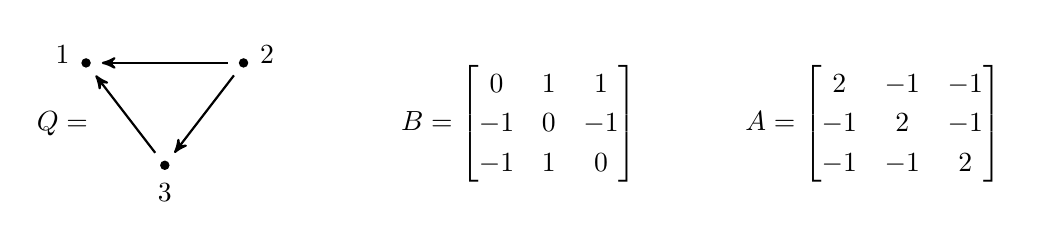
\begin{tikzpicture}
    \node (l) [matrix] at (0,0) {
      \coordinate (a) at (0,0); 
      \coordinate (b) at (2,0); 
      \coordinate (c) at (1,-1.3);
      \foreach \c in {a,b,c} {\fill (\c) circle (.06);}
      \foreach \c/\d in {b/a,b/c,c/a} {\draw[thick,-stealth',shorten <=2mm,shorten >=2mm] (\c) to (\d);}
      \node (alabel) at ($(a)+(-.3,.1)$) {1};
      \node (blabel) at ($(b)+(.3,.1)$) {2};
      \node (clabel) at ($(c)+(0,-.35)$) {3};
    \\
    };
    \node (Q) at (-1.3,0) {$Q =$};
    \node (m) at (4.5,0) {$B = \begin{bmatrix} 0 & 1 & 1 \\ -1 & 0 & -1 \\ -1 & 1 & 0 \end{bmatrix}$};
    \node (r) at (9,0) {$A = \begin{bmatrix} 2 & -1 & -1 \\ -1 & 2 & -1 \\ -1 & -1 & 2 \end{bmatrix}$};
  \end{tikzpicture}
  \caption{
    An acyclic skew-symmetric matrix $B$, its Cartan companion $A$, and the corresponding quiver $Q$. 
    The vertex labels of $Q$ correspond to the row/column labels of $B$ and $A$, and the Coxeter element associated to $B$ and $Q$ is $c = s_1 s_3 s_2$.
  }
  \label{fig:matrices}
\end{figure}  

The cluster algebra associated to an $m\times n$ acyclic exchange matrix of rank $n$ is especially well-behaved: it is finitely generated as a $\kk$-algebra and coincides with its upper cluster algebra \cite{BFZ05}.
For such cluster algebras we will concern ourself with a specific sequence of nodes in $\TT$ and the cluster variables associated to them.

Recall that $t_0$ is the root of $\TT$.  Fix an acyclic skew-symmetrizable matrix $B$ and the corresponding permutation $\sigma$ as above.
Write $t_m:m\in\ZZ$ for the nodes of $\TT$ lying along the unique path 
\begin{equation}
  \cdots
  \dashname{\sigma_n}
  t_{-n}
  \dashname{\sigma_1}
  \cdots
  \dashname{\sigma_{n-1}}
  t_{-1}
  \dashname{\sigma_n}
  t_0
  \dashname{\sigma_1}
  t_1
  \dashname{\sigma_2}
  \cdots
  \dashname{\sigma_n}
  t_n
  \dashname{\sigma_1}
  \cdots
\end{equation}
This, in general, is only a subpath in what is called the \newword{acyclic belt} (the subgraph of $\TT$ consisting of all the nodes whose attached exchange matrices are acyclic).
Indeed it is straightforward to observe that all the matrices $B^{t_m}$ are acyclic, it is less obvious but ultimately true that if $B^t$ is acyclic for some $t\in\TT$ then all cluster variables $x_{i;t}$ are realized in the above path.
\saySS{Citation needed.}\sayDR{The closest reference I know of is Cor. 4 in ``From Triangulated Categories to Cluster Algebras II'' by Caldero and Keller, though one has to look into the proof a little and note that the cluster variables in the acyclic belt sweep out the entire transjective component of the AR quiver for the cluster category.}
We will refer to the non-initial cluster variables $x_{i;t_m}$ with $m>0$ (resp. $m<0$) as \newword{preprojective} (resp. \newword{postinjective}).
This terminology will be justified in the next section.

\subsection{Quiver representations and cluster characters}\label{sec:quiverbackground}
A \newword{quiver} $Q=(Q_0,Q_1,s,t)$ with $n$ vertices consists of a set $Q_0=\{1,2,\ldots,n\}$ of vertices, a set $Q_1$ of arrows, and maps $s,t:Q_1\to Q_0$ giving the source and target of an arrow.  
A \newword{$\kk$-representation} $M=(M_i,M_a)$ of $Q$ consists of a $\kk$-vector space $M_i$ for each $i\in Q_0$ and a $\kk$-linear map $M_a:M_{s(a)}\to M_{t(a)}$ for each arrow $a\in Q_1$.  
A morphism of representation $\theta:M\to N$ consists of a collection of $\kk$-linear maps $\theta_i:M_i\to N_i$ so that $\theta_{t(a)}\circ M_a=N_a\circ \theta_{s(a)}$ for each arrow $a\in Q_1$.  
The space of all such homomorphisms will be denoted $\Hom_Q(M,N)$.

When the quiver $Q$ is \newword{acyclic} (i.e. has no oriented cycles), its category $\rep_\kk(Q)$ of finite-dimensional representations is particularly nice and thus we assume $Q$ is acyclic throughout.  
In this case, it is well-known that $\rep_\kk(Q)$ is a hereditary, abelian, length category with finitely many simple objects.  
When $Q$ is an orientation of a simply-laced finite-type Dynkin diagram, $\rep_\kk(Q)$ contains only finitely many indecomposable representations.

Write $\kk Q$ for the \newword{path algebra} of $Q$, this is the $\kk$-vector space with basis given by paths (including the trivial paths) in $Q$.  
The vector space $\kk Q$ has a multiplication given by concatenation of paths and one may identify the module category of $\kk Q$ with $\rep_\kk(Q)$, however we will not use this here.  
The path algebra $\kk Q$ is naturally considered as a representation of $Q$ where the vector space at vertex $i$ is spanned by all paths in $Q$ ending at $i$ and the action of an arrow $a$ is by concatenation.  The \newword{projective} representations of $Q$ are exactly the indecomposable summands of $\kk Q$.

Given a representation $M\in\rep_\kk(Q)$ and a projective presentation $0\to P_1\to P_0\to M\to 0$ (which may always be chosen to terminate after two terms since $\rep_\kk(Q)$ is hereditary), we define the \newword{Auslander-Reiten translate} $\tau(M)\in\rep_\kk(Q)$ via the short exact sequence
\begin{equation}\label{eq:AR translation}
  0\longrightarrow \tau(M)\longrightarrow D\Hom_Q(P_1,\kk Q)\longrightarrow D\Hom_Q(P_0,\kk Q)\longrightarrow 0,
\end{equation}
where $D=\Hom(-,\kk)$ is the standard $\kk$-linear duality functor.

The AR translation $\tau$ strongly controls the representation theory of $Q$: a representation $P$ is projective if and only if $\tau(P)=0$ while a representation $I$ is injective if and only if it is not of the form $\tau(M)$ for any $M$.  
Call a representation $M$ \newword{preprojective} if $\tau^k(M)$ is projective for some $k\ge0$, \newword{postinjective} if there is an injective representation $I$ so that $M=\tau^k(I)$ for some $k\ge0$, and \newword{regular} otherwise.  
When $Q$ is an orientation of a simply-laced finite-type Dynkin diagram, the injective representations are preprojective (hence projective representations are postinjective) and there are no regular representations.  

Write $\cQ$ for the \newword{Grothendieck group} of $\rep_\kk(Q)$ and note that $\cQ\simeq \ZZ^n$ is a free abelian group generated by the classes $[S_i]$ of the vertex-simple representations of $Q$.  
For $M\in\rep_\kk(Q)$ we thus call $[M]\in\cQ$ its \newword{dimension vector}.  
Since $\rep_\kk(Q)$ is hereditary, the \newword{Euler-Ringel form} \[\langle M,N\rangle:=\dim_\kk\Hom(M,N)-\dim_\kk\Ext^1(M,N)\] only depends on the dimension vectors of $M$ and $N$.  
In particular, the Euler-Ringel form is completely determined by the pairings of vertex-simple representations:
\[\langle S_i,S_j\rangle=\begin{cases}1 & \text{if $i=j$;}\\ -1 & \text{if $i\to j\in Q_1$;}\\ 0 & \text{otherwise.}\end{cases}\]

\saySS{Say something to the effect that $Q$ comes from $B$. Otherwise define $\mathcal{A}_Q$ somewhere.}
\saySS{I am confused here: do we allow coefficients in $\mathcal{A}_Q$? if so then we need to talk about quiver with frozen vertices, if not then we need to change the definition below and replace $m$ by $n$}
\sayDR{We should definitely allow quivers with frozen vertices and make explicit that we only care about representations supported on the principal part of the ice quiver}
If $Q$ is a finite quiver without oriented cycles, the non-initial cluster variables in $\cA_Q$ are in bijection with the rigid indecomposable representations of $Q$ \cite{CC,CK}. The bijection is given by associating to a representation $M$ a generating function encoding its submodule structure, referred to as its \newword{cluster character} or Caldero-Chapoton function. 

The definition of the cluster character involves the \newword{coindex} $\coind(M) \in \ZZ^n$, taken as an element of the weight lattice for the associated Cartan matrix (see Section~\ref{sec:group background}). If
\[
0 \to M \to \bigoplus I_j^{a_j} \to \bigoplus I_j^{b_j} \to 0
\]
is an injective resolution of $M$, then $\coind(M)$ is the element of $\ZZ^n$ whose $j$-th component is $a_j - b_j$. Below we write $x^{-\coind(M)}$ for the monomial $\prod x_j^{b_j - a_j}$. 

Given a dimension vector $e \in \NN^n$, the \newword{quiver Grassmannian} $\Gr_eM$ is the variety of $e$-dimensional submodules of $M$. We write $\chi(\Gr_eM)$ for its Euler characteristic (formally, in \'etale cohomology with compact supports), and write $\hat{y}^e$ for the monomial $\prod_j \hat{y}_j^{e_j}$, where $e_j$ is the $j$-th component of $e \in \NN^n$ and we write $\hat{y}_j$ for the monomial $\prod\limits_{i=1}^m x_i^{b_{ij}}$.

\begin{definition}
The cluster character of a representation $M$ of $Q$ is
\begin{equation}\label{eq:cc formula}
  x_M := x^{-\coind(M)} \sum_{e \in \NN^n}\chi(\Gr_e M) \hat{y}^e \in \kk[x_1^{\pm 1},\dotsc,x_m^{\pm 1}]
\end{equation}
\end{definition}

Recall that a representation $M$ of $Q$ is \newword{rigid} if $\Ext^1(M,M) = 0$. 


\begin{theorem}\label{thm:CCbijection}\cite{CC,CK}
The assignment $M \mapsto x_M$ defines a bijection between the set of rigid indecomposable representations of $Q$ and the set of non-initial cluster variables in $\cA_Q$. 
\end{theorem}

Thus we refer to non-initial cluster variables of $\cA_Q$ as preprojective, postinjective, or regular if they come from a quiver representation of the corresponding type.

*****TO DO: Characterization of these via acyclic belt.

Theorem~\ref{thm:CCbijection} generalizes to the case of skew-symmetrizable matrices by replacing quiver representations with representations of valued quivers or species. We refer to \cite{Ru15} for details, though we will not make direct use of this here. 


%\section{Kac-Moody Groups, double Bruhat cells, and generalized minors}

%\subsection{PROVISIONAL: Generalities and main theorem}
%Things to do here:
%\begin{itemize}
%  \item
%    Introduce KM goups
%  \item
%    Say we restrict to derived subgroups (mention that this is just a trick to get rid of some irrelevant coefficients and that we could do without at the cost of heavier notation) 
%  \item
%    define generalized minors
%  \item
%    recall double bruhat decomposition
%  \item
%    Decide if, for the general and preproj/postinj sections, we assume $c=s_1\cdots s_n$ and permute the rows and columns of $A$ and $B$ accordingly. 
%    If not introduce $\prec_c$ and revisit all the statements.
%    If we do not make this assumption the explicit formulas in the next subsection (together with the various proofs in the preproj/postinj section) need to be altered significantly.
%  \item
%    prove thm: $G^{c,c^{-1}}$ is upper cluster algebra with coefficients $\Delta$ (Basically cite Harold)
%  \item
%    prove prop: we can rescale coefficients to have principal. 
%    This is needed because Harold's theorem says that $\CC[G^{c,c^{-1}}]$ is a cluster algebra with a different set of coefficients.
%    Use the notation $z_i$ and $z_{-i}$ for the new coefficients.
%    The choice of having the same letter and $\pm$ indices is justified by this explicit computation
%    \begin{eqnarray}
%      z_i
%      =
%      \Delta_{c\omega_i}^{\omega_i}
%      \prod_{ j <i}\big(\Delta_{c\omega_ j }^{\omega_ j }\big)^{a_{ j  i}}
%      &=&
%      t_i
%      h^{\omega_i}\prod_{ j <i}h^{a_{ j  i}\omega_ j }\\
%      z_{-i}
%      =
%      \Delta_{\omega_i}^{c\omega_i}
%      \prod_{ j <i}\big(\Delta_{\omega_ j }^{c\omega_ j }\big)^{a_{ j  i}}
%      &=&
%      t_{-i}
%      h^{\omega_i}\prod_{ j <i}h^{a_{ j  i}\omega_ j }
%    \end{eqnarray}
%    Not having picked the letter $y$ should help to distinguish principal coefficients from doubled principal coefficients.
%    I am partially satisfied by this choice; for uniformity with cluster variables I would rather have some capital/greek capital letter for the coefficients of $\CC[G^{c,c^{-1}}]$.
%  \item
%    mention that, since the algebra is acyclic this is a cluster algebra and not just an upper cluster algebra
%  \item
%    Do we want to even mention $L^{c,c^{-1}}$?
%  \item
%    anything else?
%  \item
%    Profit
%\end{itemize}


\subsection{Kac-Moody groups and generalized minors}\label{sec:group background}

For each symmetrizable Cartan matrix $A$ there is an associated Kac-Moody group $\widehat{G}:=\widehat{G}_A$. 
It has several variants, and we consider the minimal version studied in \cite{KP83} and \cite[Sec. 7.4]{Kum02}. 
This is an ind-algebraic group whose derived subgroup $G$ is generated by coroot subgroups $\varphi_i: SL_2 \into G$ for $1 \leq i \leq n$. Starting from $G$, the larger group $\widehat{G}$ is obtained as a semidirect product with an algebraic torus of dimension equal to the corank of $A$.
%isomorphic to  $G \rtimes (\kk^\times)^{\corank(A)}$. 


When $A$ is of finite type, $G \cong \widehat{G}$ is a simply-connected semisimple algebraic group. When $A$ is of (untwisted) affine type, $G$ can be identified with the universal central extension of the group $LG^\circ$ of algebraic loops (that is, regular maps from $\kk^\times$) into some simply-connected semisimple algebraic group $G^\circ$; in this case $\widehat{G}$ is obtained by adjoining a factor of $\kk^\times$ acting by loop rotations.


For $t \in \kk^\times$ and $1 \leq i \leq n$ we adopt the notation 
\begin{gather}
x_{i}(t):=\varphi_i\begin{pmatrix} 1 & t \\ 0 & 1\end{pmatrix} \quad  
t^{\alpha_i^\vee}:=\varphi_i\begin{pmatrix}t & 0 \\ 0 & t^{-1}\end{pmatrix} \quad
x_{\ol{\imath}}(t):=\varphi_i\begin{pmatrix} 1 & 0 \\ t & 1\end{pmatrix} \\
\ol{s_{\imath}} := \varphi_i \begin{pmatrix} 0 & -1 \\ 1 & 0 \end{pmatrix} \quad
\dol{s_{i}} := \varphi_i \begin{pmatrix} 0 & 1 \\ -1 & 0 \end{pmatrix},
\end{gather}%\sayDR{Are the $\dol{s_{i}}$ needed?}\sayHW{Maybe not -- check during wrap-up}
By extension for any $w$ in the Weyl group $W$ of $\widehat{G}$ we set \[\ol{w} := \ol{s_{i_1}}\cdots\ol{s_{i_k}}, \quad \quad \dol{w} := \dol{s_{i_1}}\cdots\dol{s_{i_k}},\] where $s_{i_1}\cdots s_{i_k}$ is any reduced word for $w$. 
We write $H$ for the ($n$-dimensional) Cartan subgroup of $G$, likewise $\widehat{H}$ for the Cartan subgroup of $\widehat{G}$ (it is isomorphic to $H \times (\kk^\times)^{\corank(A)}$). We let $\kk[\widehat{G}]$ denote the (complete topological) algebra of regular functions on $\widehat{G}$.
%The Cartan subgroup $H$ of $G$ (resp. $\widehat{H}$ of $\widehat{G}$) is $n$-dimensional (resp. ($n + \corank(A)$)-dimensional). 

We have weight lattices $\widehat{P} = \Hom(\widehat{H},\kk^\times)$ and $P = \Hom(H,\kk^\times)$, and write the value of $\lambda \in P$ on $h \in H$ as $h^\lambda$ (likewise for $\lambda \in \widehat{P}$ and $h \in \widehat{H}$). The fundamental weights $\omega_1,\dotsc,\omega_n \in P$ are defined by $(t^{\alpha_i^\vee})^{\omega_j} = t^{\delta_{ij}}$. The inclusion $H \into \widehat{H}$ induces a projection $\widehat{P} \onto P$, and we fix once and for all a splitting $P \into \widehat{P}$ (this is equivalent to fixing an isomorphism $\widehat{G} \cong G \rtimes (\kk^\times)^{\corank(A)}$). Note that while $\widehat{P} \onto P$ is $W$-equivariant, the splitting will generally not be.

%We denote its ($n$-dimensional) Cartan subgroup by $H$, its standard opposite Borel subgroups by $B_\pm$, and its root and weight lattices by $Q \subset P = \Hom(H,\kk^\times)$. 
%When $A$ is of (untwisted) affine type, $G$ is the universal central extension of the group of regular maps from $\kk^\times$ to a simple algebraic group $G^\circ$. 

%The group $G$ is the derived subgroup of a larger group $\widehat{G}$, which is the semidirect product of $G$ with an algebraic torus of dimension equal to $n$ minus the rank of $A$; in the affine case this is the group that also includes a copy of $\kk^\times$ acting by loop rotations. We write $\widehat{H}$ for its Cartan subgroup (which contains $H$), $\widehat{P}$ for the extended weight lattice $\Hom(\widehat{H},\kk^\times)$, and fix once and for all a splitting $P \into \widehat{P}$ of the natural map $\widehat{P} \onto P$.

%Given a symmetrizable Cartan matrix $A$, there is an associated Kac-Moody group $G:=G_A$. 
%It has several variants, and we consider the minimal version studied in [KP]. 
%This is an ind-algebraic group generated by coroot subgroups $\varphi_i: SL_2 \into G$. 
%We denote its ($n$-dimensional) Cartan subgroup by $H$, its standard opposite Borel subgroups by $B_\pm$, and its root and weight lattices by $Q \subset P = \Hom(H,\kk^\times)$. 
%When $A$ is of (untwisted) affine type, $G$ is the universal central extension of the group of regular maps from $\kk^\times$ to a simple algebraic group $G^\circ$. 

%The group $G$ is the derived subgroup of a larger group $\widehat{G}$, which is the semidirect product of $G$ with an algebraic torus of dimension equal to $n$ minus the rank of $A$; in the affine case this is the group that also includes a copy of $\kk^\times$ acting by loop rotations. We write $\widehat{H}$ for its Cartan subgroup (which contains $H$), $\widehat{P}$ for the extended weight lattice $\Hom(\widehat{H},\kk^\times)$, and fix once and for all a splitting $P \into \widehat{P}$ of the natural map $\widehat{P} \onto P$.

Generalized minors are certain functions on $\widehat{G}$, recovering the usual notion of minors when $\widehat{G} \cong SL_n$. 
The general definition involves the representation theory of $\widehat{G}$. %This discussion involves the weight lattices $\widehat{P} = \Hom(\widehat{H},\kk^\times) \onto P = \Hom(H,\kk^\times)$, and we fix once and for all a splitting $P \into \widehat{P}$ (this is equivalent to fixing an isomorphism $\widehat{G} \cong G \rtimes (\kk^\times)^{\corank(A)}$). 
By a weight representation $V$ of $\widehat{G}$ we will always mean an algebraic representation that splits as a direct sum
\[
V = \bigoplus_{\lambda \in \widehat{P}} V_\lambda
\]
of finite-dimensional weight spaces under the action of $\widehat{H}$. Note that the weight spaces of $V$ as a $G$-representation are not necessarily finite-dimensional, as the weight decomposition of the $\widehat{H}$-action is finer than that of the $H$-action. 


%We will be interested in principal generalized minors on $G$, and to define these we recall a little representation theory. Let $P$ be the weight lattice $\Hom(H,\kk^\times)$, and $Q \subset P$ the root lattice of $G$. Let $P^+ \subset P$ denote the set of dominant weights, which are nonnegative integral combinations of the fundamental weights $\omega_1,\dotsc,\omega_n$. Each $\lambda \in P^+$ labels an irreducible highest-weight representation $L(\lambda)$ of $\widehat{G}$. This is a weight representation with finite-dimensional weight spaces; the weights that appear lie in the convex hull of the (infinite) Weyl group orbit of $\lambda$ in $P$. 

A weight $\lambda \in \widehat{P}$ is dominant if $(t^{\alpha_i^\vee})^\lambda$ is a nonnegative power of $t$ for all $1 \leq i \leq n$, and we denote the set of dominant weights by $\widehat{P}^+$. 
%The cone $\widehat{P}^+ \subset \widehat{P}$ of dominant weights consists of wei
%Let $\widehat{P}^+=\{\lambda \in \widehat{P}: \lambda(\alpha_i^\vee)>0\} \subset \widehat{P}$ denote the cone of dominant (integral) weights.  
To each $\lambda \in \widehat{P}^+$ is an associated irreducible highest-weight representation $V(\lambda)$ of $\widehat{G}$. 
Similarly, for each $\lambda \in -\widehat{P}^+$ there is an irreducible lowest-weight representation $V(\lambda)$ of $\widehat{G}$.
For any $w\in W$ and $\lambda\in\pm\widehat{P}^+$, the weight space $V(\lambda)_{w\lambda}$ is one-dimensional and thus we also write $V(w\lambda)$ for the representation $V(\lambda)$.
The Tits cone $$X = \{w\lambda : w \in W, \lambda \in \widehat{P}^+\}$$ is the set of weights which can be obtained from a dominant weight by the action of the Weyl group. 
Thus each weight $\lambda\in X \cup -X$ determines an irreducible (highest- or lowest-) weight representation $V(\lambda)$ of $\widehat{G}$ whose weight space $V(\lambda)_\lambda$ is one-dimensional.
Note that highest- and lowest-weight representations are distinct classes unless $A$ is of finite-type.

When $A$ is of (untwisted) affine type, identifying $G$ with a central extension of $LG^\circ$ fixes a splitting $P \cong P^\circ \oplus \ZZ \kappa$, %\sayDR{Should this have $\ZZ\kappa$ so that $P$ is a lattice?} 
where $P^\circ$ is the weight lattice of the underlying semisimple group $G^\circ$ and $\kk \kappa = \Hom( Z(G),\kk^\times)$.
Above this we have the splitting $\widehat{P} \cong P \oplus \ZZ \delta$, where $\delta$ is a character of the $\kk^\times$ acting by loop rotations. 
A weight $\lambda \in \widehat{P}$ is in the complement of $X \cup -X$ if and only if it lies in $P^\circ \oplus \ZZ \delta$. 
Following the above notation, for $\lambda^\circ\in P^\circ$ we have an irreducible $G^\circ$-representation $V(\lambda^\circ)$ whose highest weight is conjugate to $\lambda^\circ$ under the Weyl group of $G^\circ$. 
%For such $\lambda$, we write $V(\lambda)^\circ$ for the irreducible $G^\circ$ representation whose highest weight is conjugate to the $P^\circ$ component of $\lambda$ under the Weyl group of $G^\circ$. 
With this in hand we extend our association of an irreducible $\widehat{G}$-representation $V(\lambda)$ to all $\lambda \in \widehat{P}$: when $\lambda \in \widehat{P} \smallsetminus(X \cup -X)$ we set $V(\lambda) := V(\lambda^\circ)[z^{\pm 1}]$, \sayDR{Should we mention somewhere that all $\lambda^\circ+r\delta$ are in the same Weyl group orbit?} the space of algebraic loops in $V(\lambda^\circ)$, where $\lambda^\circ$ is the $P^\circ$-component of $\lambda$. 
The level of an irreducible $\widehat{G}$-representation is the character by which $Z(G) = Z(\widehat{G}) \cong \kk^\times$ acts; the level of $V(\lambda)$ is positive if $\lambda \in X$, negative if $\lambda \in -X$, and zero if $\lambda \in \widehat{P} \smallsetminus(X \cup -X)$. 
%or zero if $\lambda \in X$, $\lambda \in -X$, or $\lambda \in \widehat{P} \smallsetminus (X \cup -X)$, respectively.
%the level of $V(\lambda)$ is positive, negative, or zero if $\lambda \in X$, $\lambda \in -X$, or $\lambda \in \widehat{P} \smallsetminus (X \cup -X)$, respectively.

\begin{definition}\label{def:minors}
Let $V$ be a weight representation of $\widehat{G}$ and $\lambda \in \widehat{P}$ a weight for which the weight space $V_\lambda$ is one-dimensional. The principal generalized minor $\Delta_{(V,\lambda)} \in \kk[\widehat{G}]$ is the function 
\[
g \mapsto \pi_\lambda(gv_\lambda)/v_\lambda,
\]
where $\pi_\lambda:V \onto V_\lambda$ is the projection whose kernel is the direct sum of the other weight spaces, and $v_\lambda \in V_\lambda$ is any nonzero vector. When $\lambda \in X \cup -X$, or when $\widehat{G}$ is of untwisted affine type and $\lambda$ is arbitrary, we simply write $\Delta_\lambda$ for $\Delta_{(V(\lambda),\lambda)}$. When $\lambda \in \widehat{P}^+$, $\lambda' = u\lambda$, and $\lambda'' = v\lambda$, the generalized minor $\Delta^{\lambda'}_{\lambda''}$ is the function $g \mapsto \Delta_\lambda(\ol{u}^{-1}g\ol{v})$. When $\lambda \in -\widehat{P}^+$, $\lambda' = u\lambda$, and $\lambda'' = v\lambda$, then $\Delta^{\lambda'}_{\lambda''}$ is the function $g \mapsto \Delta_\lambda(\dol{u}^{-1}g\dol{v})$.
%When $\lambda \in X \cup -X$ and $\lambda' = w \lambda$, the generalized minor $\Delta^{\lambda}_{\lambda'}$ is the function $g \mapsto \Delta_\lambda(g\ol{w})$. 
%Given $\lambda \in X \cup -X$, the principal generalized minor $\Delta_\lambda \in \kk[G]$ is the function
%\[
%g \mapsto \pi_\lambda(gv_\lambda)/v_\lambda \in \kk.
%\]
%That is, its value at $g$ is a diagonal matrix coefficient in a matrix by which $g$ acts on $L(\lambda)$.
%Let $\lambda \in P^+$ be a dominant weight and $\lambda_1 = w_1\lambda$, $\lambda_2 = w_2 \lambda \in X$ be any two conjugates under the Weyl group. The 
\end{definition}

In other words, if we use a weight basis of $V$ to write the action of $g$ as a matrix, $\Delta_{(V,\lambda)}(g)$ is the diagonal entry corresponding to $V_\lambda$. Similarly, $\Delta^{\lambda'}_{\lambda''}(g)$ is the matrix entry whose row corresponds to $V_{\lambda''}$ and whose column corresponds to $V_{\lambda'}$ (up to an overall scalar fixed by the chosen representatives of $u$, $v \in G$). While we have apparently given two definitions of $\Delta^{\lambda'}_{\lambda''}$ in finite type (depending on whether we regard $\lambda'$, $\lambda''$ as conjugate to a dominant or anti-dominant weight), the reader may check that these definitions agree in this case. \sayHW{This could be made into a lemma}
\saySS{Or we could say ``this is the rationale behind of prop bla in [BFZ]''}
\sayHW{I'm not sure I understand this statement -- there are no potentially conflicting definitions presented in BFZ, so this issue does not arise}

\begin{remark}
When $\widehat{G}$ is of affine type, the representations $V(\lambda)$ with $\lambda \in \widehat{P}\smallsetminus(X \cup - X)$ are not the only irreducible level zero weight representations. The set of all such representations is parametrized by pairs $(\{\lambda_1,\dotsc,\lambda_m\},\{a_1,\dotsc,a_m\})$ of a tuple of dominant weights of $G^\circ$ and a tuple of elements of $\kk^\times$ \cite{CP86}. As a vector space the associated representation is the space of Laurent polynomials valued in the tensor product of the $V(\lambda_i^\circ)$, and the scalars $a_i$ rescale the action of $G^\circ$-valued loops on each factor.
\end{remark}

A crucial feature of generalized minors is the following generalized determinantal identity:

\begin{proposition}\cite{FZ99,Wil13}
  \label{prop:fundid}
  Suppose $u,v \in W$ and $1 \leq i \leq n$ are such that $\ell(u)<\ell(us_i)$ and $\ell(v)<\ell(vs_i)$. 
  Then 
  \begin{equation}
    \label{eq:fundid}
    \Delta_{u\omega_i}^{v\omega_i} \Delta_{us_i\omega_i}^{vs_i\omega_i} 
    =
    \prod_{\stackrel{1\leq j \leq n}{j\neq i}}\left(\Delta_{u\omega_j}^{v\omega_j}\right)^{-a_{ji}}
    +
    \Delta_{us_i\omega_i}^{v\omega_i} \Delta_{u\omega_i}^{vs_i\omega_i}
  \end{equation}
is satisfied on $G$.
\end{proposition}

While the above identity on $G$ is the one we use directly, we note that it restricts from a similar one on $\widehat{G}$ that also involves the characters of $\widehat{G}/G$.

\subsection{Acyclic cluster algebras from double Bruhat cells}

The data of an $n\times n$ acyclic skew-symmetrizable matrix $B$ is equivalent to the data of a symmetrizable Cartan matrix $A$ (the \newword{Cartan companion} of $B$) together with a reduced word $(\sigma_1,\ldots,\sigma_n)$ for a Coxeter element $c$ of its Weyl group.
The Cartan matrix is obtained from $B$ by making all its entries negative without changing their absolute values, then setting each diagonal entry equal to two; see Figure~\ref{fig:matrices}.
The reduced word $(\sigma_1,\ldots,\sigma_n)$ for $c$ is equivalent to a permutation $\sigma \in S_n$ which satisfies the following property: $b_{\sigma_i \sigma_j} \geq 0$ when $i < j$, such a permutation exists since $B$ is acyclic (choosing a different permutation with the above property defines the same Coxeter element via a different reduced word).
Conversely, any acyclic skew-symmetrizable matrix can be obtained from a Cartan matrix and a reduced word for a Coxeter element $c$ by assigning signs to the off-diagonal entries of $B$ according to the reduced word of $c$.

We can realize the cluster algebra associated to the acyclic matrix $B$ geometrically in terms of the Kac-Moody group $G$ associated to $A$. More precisely, through the group we naturally find the algebra associated to the exchange matrix
\[
\Bdp := \begin{bmatrix} B \\ Id_n \\ Id_n \end{bmatrix},
\]
which we say has \newword{doubled principal coefficients}. When working with the cluster algebra $\cA_{\Bdp}$ we will denote the frozen variables $x_{i+n}$ and $x_{i+2n}$ for $1 \leq i \leq n$ by $z_i$ and $z_{\ol{\imath}}$, respectively

%The goal of this section is to realize geometrically the ``doubled principal coefficients'' cluster algebra $\cA_{\widetilde B_{\doublebullet}}$, given by the $3n\times n$ extensions $\widetilde B_{\doublebullet}$ of $B$ by two identity matrices, in terms of the derived Kac-Moody group $G$ associated to $A$. 
%\saySS{Giovanni suggested to use two bullets one on top of the other for doubled principal coefficients. The standard notation for principal coefficients is a single bullet so it sounded like a good idea to stack two bullets.}
%To emphasize that we get two copies of each frozen cluster variable, and to suggestively record their values, we will denote $x_{i+n}$ and $x_{i+2n}$ by $z_i$ and $z_{-i}$, respectively for $1 \leq i \leq n$. 

We recall the double Bruhat decomposition
\[
G = \bigsqcup_{u,v \in W} G^{u,v},\quad G^{u,v} : = B_+ u B_+ \cap B_- v B_-
\]
of $G$, where $B_{\pm}$ are the standard opposite Borel subgroups of $G$. 
Each $G^{u,v}$ is a smooth affine variety of dimension $n + \ell(u) + \ell(v)$, where $\ell(u)$, $\ell(v)$ are the lengths of $u$ and $v$ \cite{FZ99,Wil13}. 
The coordinate ring of $G^{u,v}$ is an upper cluster algebra and a finite subset of its clusters are in correspondence with shuffles of reduced words for $u$ and $v$ \cite{BFZ05,Wil13}. 
\begin{remark}
Each $G^{u,v}$ is the intersection of $G \subset \widehat{G}$ with the double Bruhat cell $\widehat{G}^{u,v}$ of $\widehat{G}$. 
The coordinate ring of the latter is also an upper cluster algebra whose initial exchange matrix has the same principal part, but with $\corank(A)$ additional frozen variables: $G^{u,v}$ is the locus where these are equal to one.
\end{remark}

\begin{theorem}
  \label{thm:coordring}
  Let $B$ be an acyclic skew-symmetrizable matrix, $G$ the Kac-Moody group of its Cartan companion $A$, and $c$ the associated Coxeter element. 
  There is an isomorphism $\cA_{\Bdp} \cong \kk[G^{c,c^{-1}}]$ that identifies the initial cluster variables with restrictions of the following monomials in generalized minors
  \begin{equation}
    \label{eq:initialcluster}
    x_i = \Delta_{\omega_i},
    \quad 
    z_i = \Delta^{\omega_i}_{ c\omega_i} \prod_{j < i}(\Delta^{\omega_j}_{c \omega_j})^{a_{ji}},
    \quad 
    z_{\ol{\imath}} = \Delta^{c \omega_i}_{\omega_i} \prod_{j < i}(\Delta^{c \omega_j}_{\omega_j})^{a_{ji}}.
  \end{equation}
\end{theorem}
\begin{proof}
  Specializing \cite[Theorem 2.10]{BFZ05} and \cite[Theorem 4.9]{Wil13} to the case at hand we get that $\kk[G^{c,c^{-1}}]$ is the upper cluster algebra with initial cluster variables $\Delta_{\omega_i}$, frozen variables $\Delta_{c\omega_i}^{\omega_i}$ and $\Delta_{\omega_i}^{c\omega_i}$, and initial exchange matrix obtained by extending $B$ with two copies of the matrix $1-[B]_+$ (here we denote by $1$ the identity matrix and we apply $[\,\cdot\,]_+$ entrywise).
  \saySS{BIG FAT WARNING: the two theorems use opposite conventions for associating an exchange matrix to a double reduce word! My feeling is that we should say much more in the proof of this theorem but I have no clue on how to do it and still sweep under the rug the issue with conventions.}

  This exchange matrix is acyclic by hypothesis and has full rank.  Thus, following \cite[Corollary 1.19]{BFZ05}, $\kk[G^{c,c^{-1}}]$ is a cluster algebra.

  The cluster structure we obtain in this way is not quite the one in the statement of the theorem; the two are nonetheless strictly related. 
  Indeed, since the variables $z_i$ are obtained from the minors $\Delta^{\omega_j}_{ c\omega_j}$ by an invertible monomial transformation (and the variables $z_{\ol{\imath}}$ are obtained similarly from the minors $\Delta^{c \omega_j}_{\omega_j}$), we can use separation of additions to rescale all the cluster variables in $\kk[G^{c,c^{-1}}]$ and establish the desired isomorphism (Cf. \cite[Proposition 4.5]{YZ08}).
  \saySS{The proof of this theorem should now be correct but I am quite unhappy because it is vague and it uses some results without recalling all the required details. Can you improve what I did in any way?}
\end{proof}
\begin{remark}
  One could consider the $2n$-dimensional subvariety $L^{c,c^{-1}} \subset G^{c,c^{-1}}$ where $z_{\ol{1}},\dotsc,z_{\ol{n}}$ are equal to one; this is the reduced double Bruhat cell studied in \cite{YZ08}. 
  In particular, $\kk[L^{c,c^{-1}}]$ is the cluster algebra with principal coefficients associated to $B$, and our results immediately translate to statements in the principal coefficients case by specializing $z_{\ol{1}},\dotsc,z_{\ol{n}}$ to one. 
%While this has a prominent role from the cluster algebra point of view, we prefer to work with doubled principal coefficients not to break the symmetry in the definition of the variety at hand.
%All our results restrict to the principal coefficients case by specializing $z_{-1},\dotsc,z_{-n}$ to one.
\end{remark}

\saySS{Shall we move this to section 3?}\sayHW{I don't feel too strongly, but stating this first here and then referencing it in section 3 makes sense to me in that this is indeed background material} 
In computing various relations in $\kk[G^{c,c^{-1}}]$ we will make extensive use of the fact that a generic element $g$ of $G^{c,c^{-1}}$ can be factored as
\begin{equation}
  \label{eq:generic_element}
  g=x_{\ol{\sigma_1}}(t_{\ol{1}}) \cdots x_{\ol{\sigma_n}}(t_{\ol{n}}) h x_{\sigma_n}(t_n) \cdots x_{\sigma_1}(t_1)
\end{equation}
for some $h \in H$ and $t_i, t_{\ol{\imath}} \in \kk^\times$ \cite{FZ99,Wil13}. 
For example, with respect to such a factorization it is clear that we have $\Delta_\lambda(g) = h^\lambda$ for any dominant weight $\lambda \in \widehat{P}^+$.
In particular, the initial mutable cluster variables of $\cA_{\Bdp}$ evaluate as $x_i(g)=h^{\omega_i}$.
Some similar computations are collected in Lemma~\ref{lemma:coefficients_values}. 
%Here we write 
%\begin{equation}
%  x_{-i}(t):=\varphi_i\left(\begin{array}{cc}1 & 0 \\ t & 1\end{array}\right)
%  \quad
%  \quad
%  x_i(t):=\varphi_i\left(\begin{array}{cc}1 & t \\ 0 & 1\end{array}\right)
%\end{equation}
%and for $t \in \kk^\times$
%\begin{equation}
%  t^{\alpha_i^\vee}:=\varphi_i\left(\begin{array}{cc}t & 0 \\ 0 & t^{-1}\end{array}\right)
%\end{equation}

%\saySS{This should cover all the minors we care about; please correct me if I am mistaken}
%Given $u,v\in W$ and $\lambda$ a weight, we denote by $\Delta_{u\lambda}^{v\lambda}$ the matrix coefficient 
%\begin{equation}
%  \Delta_{u\lambda}^{v\lambda}(g) 
%  := 
%  \left(\left[ \overline{u}^{-1}g\overline{v} \right]_0\right)^\lambda
%\end{equation}
%When $u=v$ above, we will write $\Delta_{u\lambda}$ instead of $\Delta_{u\lambda}^{u\lambda}$.

%\begin{proposition}\say[Group]{We need to think carefully about the change of coefficents, keeping in mind [Yang-Zelevinsky: p. 21] at the end of Sec. 4 and [Berenstein-Rupel: Lemma 6.8].}

%\begin{proposition}
%Let $G$ be a Kac-Moody group, let $c$ be a Coxeter element of its Weyl group, and $B_c$ the associated exchange matrix.  The coordinate ring of the double Bruhat cell $G^{c,c^{-1}}$ is an upper cluster algebra of type $B_c$ with coefficients.  The coordinate ring of the reduced double Bruhat cell $L^{c,c^{-1}}$ is an upper cluster algebra of type $B_c$ with principal coefficients.
%\end{proposition}
%\begin{proof}
%\begin{enumerate}
%\item Cite other papers.
%\item Generalities on reducing double Bruhat cells and forgetting coefficients.
%\item Redo Yang-Zelevinsky change of coefficients.
%\end{enumerate}
%\end{proof}

%\begin{proposition}
%Let $G$ be a Kac-Moody group, let $c$ be a Coxeter element of its Weyl group, and $B_c$ the associated exchange matrix.  All initial and preprojective cluster variables in the coordinate ring of $G^{c,c^{-1}}$ are restrictions of principal minors of highest weight representations.  Their $g$-vectors are of the form $\dotsc$, and the cluster variable with $g$-vector $g = (g_1,\dotsc,g_n)$ is the restriction of the principal minor of weight $\sum g_i \omega_i$.
%\end{proposition}
%\begin{proof}
%\begin{enumerate}
%\item Redo Yang-Zelevinsky computation of the exchange relations among preprojective minors.
%\end{enumerate}
%\end{proof}

%\begin{proposition}
%Let $G$ be a Kac-Moody group, let $c$ be a Coxeter element of its Weyl group, and $B_c$ the associated exchange matrix.  All postinjective cluster variables in the coordinate ring of $G^{c,c^{-1}}$ are restrictions of principal minors of lowest weight representations.  Their $g$-vectors are of the form $\dotsc$, and the cluster variable with $g$-vector $g = (g_1,\dotsc,g_n)$ is the restriction of the principal minor of weight $\sum g_i \omega_i$.
%\end{proposition}
%\begin{proof}
%\begin{enumerate}
%\item Compute change of coordinates between oppositely shuffled parametrizations.
%\item Use this to show antifundamental minors are mutations of fundamental ones.
%\item Think about coefficients in oppositely shuffled parametrization.
%\item Show negative version of generalized minor identities reduce to exchange relations among postinjective minors.
%\end{enumerate}
%\end{proof}


%\subsection{Explicit computations}
%\saySS{This subsection is written assuming $c=s_1\cdots s_n$}
%\saySS{the rationale of this subsection is to introduce the notation for the generic element of $G^{c,c^{-1}}$ that we use in both the preproj/postinj and the regular sections. With the excuse, having showed that we have a cluster algebra by pinpointing generalized minors it sounds like a good idea to say what are they.}
%For later use we record here the values that both the initial cluster variables and the coefficients of $\CC[G^{c,c^{-1}}]$ assume on the generic element of $G^{c,c^{-1}}$.
%In most cases to obtain these formulas it suffices to perform a straightforward computation in the relevant representation (either $L_{\omega_i}$ or $L_{-\omega_i}$) so we will omit proofs.

%For $i\in[1,n]$ let $\varphi_i:SL_2\rightarrow G$ denote the canonical embedding corresponding to the simple root $\alpha_i$. 
%For $t\in\CC$ 
%Here we write 
%\begin{equation}
%  x_{-i}(t):=\varphi_i\left(\begin{array}{cc}1 & 0 \\ t & 1\end{array}\right)
%  \quad
%  \quad
%  x_i(t):=\varphi_i\left(\begin{array}{cc}1 & t \\ 0 & 1\end{array}\right)
%\end{equation}
%and for $t \in \kk^\times$
%\begin{equation}
%  t^{\alpha_i^\vee}:=\varphi_i\left(\begin{array}{cc}t & 0 \\ 0 & t^{-1}\end{array}\right)
%\end{equation}
%so that the generic element of $G^{c,c^{-1}}$ is
%\begin{equation}
%  \label{eq:generic_element}
%  g=x_{-1}(t_{-1}) \cdots x_{-n}(t_{-n}) h x_n(t_n) \cdots x_1(t_1)
%\end{equation}
%with $h\in H$ and $t_{\pm i} \in \CC$ (cf. \cite[Proposition 3.2]{Wil13} were we prefer to place the torus part in central position using the classical commutation relations \cite[(2.5)]{FZ99}).

%\begin{lemma}
%  \label{lemma:initial_cluster_variables}
%  On the generic element $g$ of $G^{c,c^{-1}}$ expressed as in \Cref{eq:generic_element} the initial cluster variables of $\CC[G^{c,c^{-1}}]$ assume the following values:
%  \begin{equation}
%    \Delta_{\omega_i}(g) = h^{\omega_i}
%  \end{equation}
%\end{lemma}

%Keeping in mind that for any $k\geq0$ the word $c^k$ is reduced (cf. \cite{Spe09}), we also get the following.

%\begin{lemma}
%  \label{lemma:coefficient_computations}
%  On the generic element $g$ of $G^{c,c^{-1}}$ expressed as in \Cref{eq:generic_element} the following can be computed explicitly for any $k\geq 0$:
%  \begin{eqnarray}
%    \Delta^{c^{k+1}\omega_j}_{c^k\omega_j}(g) &=& h^{c^k\omega_j}\prod_{i=1}^n t_{-i}^{[c^k\beta_j^+:\alpha_i]}\\
%    \Delta^{c^k\omega_j}_{c^{k+1}\omega_j}(g) &=& h^{c^k\omega_j}\prod_{i=1}^n t_{i}^{[c^%k\beta_j^+:\alpha_i]}\\
%    \Delta^{-c^{-k-1}\omega_j}_{-c^{-k}\omega_j}(g) &=& h^{-c^{-k-1}\omega_j}\prod_{i=1}^n% t_{i}^{[c^{-k}\beta_j^-:\alpha_i]}\\
%    \Delta^{-c^{-k}\omega_j}_{-c^{-k-1}\omega_j}(g) &=& h^{-c^{-k-1}\omega_j}\prod_{i=1}^n% t_{-i}^{[c^{-k}\beta_j^-:\alpha_i]}
%  \end{eqnarray}
%\end{lemma}

%Finally we can explicitly compute the value of $z_i$ and $z_{-i}$.
%\begin{lemma}
%  \label{lemma:coefficients_values}
%  On the generic element $g$ of $G^{c,c^{-1}}$ expressed as in \Cref{eq:generic_element} we can explicitly compute
%  \begin{eqnarray}
%    z_i(g)
%    &=&
%    t_i
%    h^{\omega_i}\prod_{ j <i}h^{a_{ j  i}\omega_ j }\\
%    z_{-i}(g)
%    &=&
%    t_{-i}
%    h^{\omega_i}\prod_{ j <i}h^{a_{ j  i}\omega_ j }
%  \end{eqnarray}
%\end{lemma}
%\begin{proof}
%  We will only concern ourself with the first identity, the other being derived% exactly in the same way.
%  Recall the definition of $z_i$
%  \saySS{Add the relevant reference once it is in place}
%  \[
%    z_i 
%    =
%    \Delta_{c\omega_i}^{\omega_i}
%    \prod_{ j <i}\big(\Delta_{c\omega_ j }^{\omega_ j }\big)^{a_{ j  i}}
%  \]
%  and substitute the values computed in \Cref{lemma:coefficient_computations} to get
%  \[
%    z_i(g)
%    =
%    \left(h^{\omega_i}\prod_{\ell =1}^n t_{\ell}^{[\beta_i^+:\alpha_\ell]}\right)
%    \prod_{j<i}\left(h^{\omega_j}\prod_{\ell=1}^n t_{\ell}^{[\beta_j^+:\alpha_\ell]}\right)^{a_{ji}}.
%  \]
%  To establish our result we need to verify that
%  \saySS{This should be changed to Harold's boolean notation}
%  \[
%    [\beta_i^+:\alpha_\ell]+\sum_{j<i}a_{ji}[\beta_j^+:\alpha_\ell]
%    =
%    \begin{cases}
%      1 & \text{ if $i=\ell$}\\
%      0 & \text{ otherwise.}
%    \end{cases}
%  \]
%  Summing up over $\ell$ we get
%  \[
%    \beta_i^++\sum_{j<i}a_{ji}\beta_j^+
%    =
%    \alpha_i
%  \]
%  which holds by telescoping.
%\end{proof}

%%%%%%%%%%%%%%%%%%%%%%%%%%%%%%%%%%%%%%%%%%%%%%
\section{Preprojective and postinjective cluster variables as minors}
In this section we prove that when $B$ is any acyclic skew-symmetrizable matrix, the identification $\cA_{\Bdp} \cong \kk[G^{c,c^{-1}}]$ of \Cref{thm:coordring} realizes preprojective and postinjective cluster variables as restrictions of some highest- and lowest-weight minors, respectively. 
For our argument we will first deduce a parametrization of such cluster variables, together with a list of exchange relations they satisfy, from an explicit description of all the $\bfg$-vectors and $\bfc$-vectors in the acyclic belt.
The identification with minors will then follow by comparing these relations with restrictions  to $G^{c,c^{-1}}$ of the generalized determinantal identities of \Cref{prop:fundid}.

\subsection{Cluster variables in the bipartite belt}
\label{sec:bipartite_belt}
Recall from the definition of acyclic matrix that there exists $\sigma\in S_n$ such that $b_{\sigma_i,\sigma_j}\geq 0$ whenever $i<j$. 
To simplify our notation, in this section, we will assume that $\sigma$ is the identity permutation by relabelling rows and columns of $B$ as needed.
Moreover, since our claim is already established in \cite{YZ08} for the simply-connected semisimple group case,  we will also assume that the Cartan companion $A$ of $B$ is not of finite type.
\saySS{For uniformity, if you want, we could cover also finite type here if we use $w_0$ in place of $c^\infty$. It is not clear to me that it is worth doing even though it will make life more uniform. Maybe we should add a comment here.}

In view of these assumptions, the Coxeter element associated to $B$ is $c=s_1\cdots s_n$ and any prefix of the word $c^\infty$ is reduced (cf. \cite{Spe09}). 
Therefore the acyclic belt becomes
\begin{equation}
  \cdots
  \dashname{n}
  t_{-n}
  \dashname{1}
  \cdots
  \dashname{n-1}
  t_{-1}
  \dashname{n}
  t_0
  \dashname{1}
  t_1
  \dashname{2}
  \cdots
  \dashname{n}
  t_n
  \dashname{1}
  \cdots
\end{equation}
\saySS{We should probably comment on the fact that all these nodes of the exchange graph are distinct. It follows from the propositions we are about to prove but one might wonder whether the argument is circular here.}
\sayDR{I think the proposition below establishes this fact, I did not see any point where you assumed they were distinct in the proof.}
Following \cite{FZ02}, we denote by $\mod{m}$ the unique integer in $[1,n]$ congruent to $m$ modulo $n$.
The edge immediately to the left of $t_m$ is then labelled by $\mod{m}$.
Observe that the nodes of $\TT$ we are considering lie along a \emph{sink/source adapted sequence}.  
More precisely, the $\mod{m}$-th row of $B^{t_m}$ contains only non-positive entries and the $\mod{m+1}$-st row only non-negative entries.
In particular, the mutation relations \eqref{eq:matrix mutation} imply that the off-diagonal entries of the exchange matrix $B^{t_m}$ are equal, in absolute value, to the entries of $A$.

We begin our analysis with a computation of $\bfc$-vectors by interpreting them as coordinate vectors in the basis of simple roots for the root system of the Cartan companion $A$.  This calculation will start by taking the $i$-th $\bfc$-vector at $t_0$ is $\alpha_i$.
\begin{lemma}
  \label{lemma:c-vectors}
  Let $\alpha_{i;t_m}$ be the $i$-th $\bfc$-vector at vertex $t_m$.
  Then
  \begin{equation}
    \alpha_{i;t_m}
    =
    \begin{cases}
      c^{\left\lfloor\frac{m-1}{n}\right\rfloor}s_1\cdots s_{\mod{m}} \alpha_i & \text{if $0<m$;}\\
      \alpha_i & \text{if $-n\leq m \leq 0$ and  $i\leq n+m$;} \\
      -\alpha_i & \text{if $-n\leq m \leq 0$ and $n+m<i$;} \\
      -c^{1+\left\lceil\frac{m+1}{n}\right\rceil}s_n\cdots s_{\mod{m+1}} \alpha_i & \text{if $m<-n$;}\\
    \end{cases}
  \end{equation}
  where, as usual, $\left\lfloor a \right\rfloor$ is the greatest integer smaller than or equal to $a$ while $\left\lceil a \right\rceil$ is the smallest integer greater than or equal to $a$.
  Moreover, whenever $m > 0 $ or $m < -n$, the vector $\alpha_{\mod{m};t_m}$ is negative and the vector $\alpha_{\mod{m+1};t_m}$ is positive.
\end{lemma}

\begin{remark}
  If $m>0$ then $c^{\left\lfloor\frac{m-1}{n}\right\rfloor}s_1\cdots s_{\mod{m}}$ is the prefix of $c^\infty$ of length $m$.
  \saySS{Reminder: for $m>0$ we write $m=\left\lfloor\frac{m-1}{n}\right\rfloor n + \mod{m}$.}
  Similarly, if $m<-n$, then $c^{1+\left\lceil\frac{m+1}{n}\right\rceil}s_n\cdots s_{\mod{m+1}}$ is the prefix of $c^{-\infty}$ of length $-m-n$.
  \saySS{Reminder: for $m<-n$ we write $-m-n =-\left(\left\lceil\frac{m+1}{n}\right\rceil+1\right)n+\mod{n-\mod{m}}$}
\end{remark}

\begin{proof}
  \saySS{I should remember to thank Anna and Pavel for hints on reflection groups}
  Let's begin by settling the claim about signs. 
  When $m>0$ the root $c^{\left\lfloor\frac{m-1}{n}\right\rfloor}s_1\cdots s_{\mod{m}} \alpha_{\mod{m+1}}$ is positive: being a prefix of $c^\infty$, the word  $c^{\left\lfloor\frac{m-1}{n}\right\rfloor}s_1\cdots s_{\mod{m}} s_{\mod{m+1}}$ is reduced (cf. \cite{Spe09}) and we can apply \cite[VI \S 1.6 Corollary 2 to Proposition 17]{Bou02}.
  By the same principle the root $c^{\left\lfloor\frac{m-1}{n}\right\rfloor}s_1\cdots s_{\mod{m}} \alpha_{\mod{m}} = -c^{\left\lfloor\frac{m-1}{n}\right\rfloor}s_1\cdots s_{\mod{m-1}} \alpha_{\mod{m}}$ is negative because the word $c^{\left\lfloor\frac{m-1}{n}\right\rfloor}s_1\cdots s_{\mod{m}}$ is reduced.
  Similarly, when $m<-n$ the root $-c^{1+\left\lceil\frac{m+1}{n}\right\rceil}s_n\cdots s_{\mod{m+1}} \alpha_{\mod{m+1}}$ is positive and the root $-c^{1+\left\lceil\frac{m+1}{n}\right\rceil}s_n\cdots s_{\mod{m+1}} \alpha_{\mod{m}}$ is negative.
  
  For the main claim there are three cases to consider.

  \noindent{\bf Case $-n \leq m \leq 0$.}
  We proceed by induction on $m$.
  For $m=0$ there is nothing to check.
  By construction, while the sign of $\alpha_{\mod{m};t_m}$ is positive, the sign of the $\mod{m}$-th row of $B^{t_m}$ is negative. 
  The $\bfc$-vectors at $t_{m-1}$ are therefore given by:
  \begin{equation*}
    \alpha_{i;t_{m-1}}
    =
    \begin{cases}
      \alpha_{i;t_m} & \text{if $i\neq \mod{m}$}\\
      -\alpha_{\mod{m};t_m} & \text{if $i = \mod{m}$}
    \end{cases}
  \end{equation*}
  as desired.

  \noindent{\bf Case $m > 0$.}
  We again argue by induction on $m$ the base case still being $m=0$. 
  Since the sign of $\alpha_{\mod{m+1};t_m}$ and the sign of the $\mod{m+1}$-st row of $B^{t_m}$ are both positive, in view of \cite[Proposition 1.3]{NZ12}, the $\bfc$-vectors at $t_{m+1}$ are given by
  \begin{align*}
    \alpha_{i;t_{m+1}} 
    &= 
    \alpha_{i;t_m} - a_{\mod{m+1},i} \alpha_{\mod{m+1};t_m}\\
    &=
    \alpha_{i;t_m} - \frac{2(\alpha_{\mod{m+1}},\alpha_i)}{(\alpha_{\mod{m+1}},\alpha_{\mod{m+1}})} \alpha_{\mod{m+1};t_m}\\
    &=
    \alpha_{i;t_m} - \frac{2(\alpha_{\mod{m+1};t_m},\alpha_{i;t_m})}{(\alpha_{\mod{m+1};t_m},\alpha_{\mod{m+1};t_m})} \alpha_{\mod{m+1};t_m}\\
    &=
    s_{\alpha_{\mod{m+1};t_m}}\big(\alpha_{i;t_m}\big)
  \end{align*}
  where the second to last equality holds because the pairing $(\cdot,\cdot)$ is invariant under the action of the Weyl group.  
  Using the inductive hypotheses we can then conclude
  \begin{align*}
    \alpha_{i;t_{m+1}} 
    &=
    s_{\alpha_{\mod{m+1};t_m}}\big(\alpha_{i;t_m}\big)\\
    &=
    \big(c^{\left\lfloor\frac{m-1}{n}\right\rfloor}s_1\cdots s_{\mod{m}}\big)s_{\mod{m+1}}\big(s_{\mod{m}}\cdots s_1 c^{-\left\lfloor\frac{m-1}{n}\right\rfloor}\big)\big(c^{\left\lfloor\frac{m-1}{n}\right\rfloor}s_1\cdots s_{\mod{m}}\alpha_i\big)\\
    &= 
    c^{\left\lfloor\frac{m-1}{n}\right\rfloor}s_1\cdots s_{\mod{m}}s_{\mod{m+1}} \alpha_i.
  \end{align*}

  \noindent{\bf Case $m < -n$.}
  The argument is the same as the one used in the case $m>0$ with $m=-n$ as base for the induction. 
  The only minor change is that this time we leverage the fact that both the sign of $\alpha_{\mod{m};t_m}$ and the sign of the $\mod{m}$-th row of $B^{t_m}$ are negative.
\end{proof}

In analogy to what we did for $\bfc$-vectors, we will interpret $\bfg$-vectors as coordinate vectors in the basis of fundamental weights for the root system of $A$ so that the $i$-th $\bfg$-vector at $t_0$ is $\omega_i$.
From \Cref{lemma:c-vectors}, in view of \Cref{eq:g-vectors_from_c-vectors} and recalling that weights are the dual basis to coroots, we immediately deduce the following.
\saySS{I can be more explicit here and say that the Cartan companion of $-B^T$ is $A^T$ which is the dual Cartan matrix. Hence we need to consider the dual basis coroots and weights. Do you want to say this much?}

\begin{lemma}
  \label{lemma:g-vectors}
  Let $\lambda_{i;t_m}$ be the $i$-th $\bfg$-vector at $t_m$. 
  Then
  \begin{equation}
    \lambda_{i;t_m}
    =
    \begin{cases}
      c^{\left\lfloor\frac{m-1}{n}\right\rfloor}s_1\cdots s_{\mod{m}} \omega_i & \text{if $m>0$;}\\
      \omega_i & \text{if $-n\leq m \leq 0$ and  $i\leq n+m$;} \\
      -\omega_i & \text{if $-n\leq m \leq 0$ and $i>n+m$;} \\
      -c^{1+\left\lceil\frac{m+1}{n}\right\rceil}s_n\cdots s_{\mod{m+1}} \omega_i & \text{if $m <-n$.}\\
    \end{cases}
  \end{equation}
\end{lemma}

With the preceding results in hand, we are ready to describe the cluster variables of $\cA_{\Bdp}$ attached to the acyclic belt.

\saySS{Is this a theorem or a proposition?}
\begin{theorem}
  \label{thm:vars_and_rels_in_bipartite_belt}
  The preprojective and postinjective cluster variables of $\cA_{\Bdp}$ are parametrized by the sets of $\bfg$-vectors
  \[
    \Pi_{\textit{proj}}:=\big\{c^k\omega_i: i \in [1,n], k>0\big\}
  \]
  and
  \[
    \Pi_{\textit{inj}}:=\big\{-c^{-k}\omega_i: i \in [1,n], k\geq0 \big\}
  \]
  respectively; we will therefore denote them by $x_{c^k\omega_i}$ and $x_{-c^{-k}\omega_i}$.

  Together with the initial cluster variables, they satisfy the following exchange relations:
  \begin{align}
    x_{c^k\omega_i}x_{c^{k+1}\omega_i} 
    &= 
    \prod_{j<i} x_{c^{k+1}\omega_j}^{-a_{ji}}
    \prod_{j>i} x_{c^k\omega_j}^{-a_{ji}}
    +
    \prod_{j=1}^n (z_j z_{\ol{\jmath}})^{[c^k\beta_i^+:\alpha_j]}\label{eq:preprojective}
    \\
    x_{-c^{-k}\omega_i}x_{-c^{-k-1}\omega_i} 
    &= 
    \prod_{j<i} x_{-c^{-k}\omega_j}^{-a_{ji}}
    \prod_{j>i} x_{-c^{-k-1}\omega_j}^{-a_{ji}}
    +
    \prod_{j=1}^n (z_j z_{\ol{\jmath}})^{[c^{-k}\beta_i^-:\alpha_j]}\label{eq:postinjective}
    \\
    x_{\omega_i}x_{-\omega_i}
    &=
    z_iz_{\ol{\imath}}
    \prod_{j<i} x_{\omega_j}^{-a_{ji}}
    \prod_{j>i} x_{-\omega_j}^{-a_{ji}}
    +
    1\label{eq:plusminus}
  \end{align}
\end{theorem}
\begin{proof}
  The first part of our claim follows immediately from \Cref{lemma:g-vectors}: it suffices to recall how simple reflections act on fundamental weights and to observe that, the type of $A$ being not finite, all prefixes of $c^\infty$ are reduced expressions so that all the elements of $\Pi_{\textit{proj}}$ and $\Pi_{\textit{inj}}$ are distinct.

  For the second part recall that $\beta_i^+=s_1\cdots s_{i-1}\alpha_i$ and $\beta_i^-=s_n\cdots s_{i+1}\alpha_i$. 
  \saySS{Were the $\beta_\pm$ defined before?}
  The relations are then an obvious consequence of \Cref{lemma:c-vectors} once we observe that mutations happen along a sink/source adapted sequence so that the $\mod{m}$-th column of $B^{t_m}$ contains only non-negative entries and the $\mod{m+1}$-th column only non-positive entries. 
\end{proof}
\begin{remark}
  As noted before, to obtain the exchange relations in the cluster algebra $\cA_{\Bpr}$ with principal coefficients it suffices to set the coefficients $z_{\ol{1}},\dotsc,z_{\ol{n}}$ to $1$ in the relations of \Cref{thm:vars_and_rels_in_bipartite_belt}. 
\end{remark}
\saySS{Somewhere we should make a trivial remark: if $n=2$ then preprojective and postinjective cluster variables are all the cluster variables}
\subsection{Highest- and lowest-weight minors}

Before proving the main result of the section, Theorem~\ref{thm:mainirregular}, we collect some lemmas concerning restrictions of minors to $G^{c,c^{-1}}$. All of the arguments involved are straightforward generalizations of those in \cite{YZ08} to the infinite-type case. 

The first lemma computes the evaluations of various minors of interest in terms of the factorization of a generic element of $G^{c,c^{-1}}$ into one-parameter subgroups. We recall that, for any root $\beta \in Q$, we let $[\beta:\alpha_i]$ denote the $i^{th}$ coefficient in the expansion
\[
\beta = \sum_{i = 1}^n [\beta:\alpha_i]\alpha_i.
\]
The roots to which we apply this notation are $\beta_i^+=s_1\cdots s_{i-1}\alpha_i$, $\beta_i^-=s_n\cdots s_{i+1}\alpha_i$, and their conjugates. We also recall that the initial cluster variables in $\kk[G^{c,c^{-1}}]$ are 
\[
x_i = \Delta_{\omega_i},\quad z_i = \Delta^{\omega_i}_{ c\omega_i} \prod_{j < i}(\Delta^{\omega_j}_{c \omega_j})^{a_{ji}},\quad z_{\ol{\imath}} = \Delta^{c \omega_i}_{\omega_i} \prod_{j < i}(\Delta^{c \omega_j}_{\omega_j})^{a_{ji}},
\]
for $1 \leq j \leq n$.

\begin{lemma}\label{lemma:coefficients_values}
If $g \in G^{c,c^{-1}}$ factors as
\begin{equation}\label{eq:generic_factorization}
g = x_{\ol{1}}(t_{\ol{1}}) \cdots x_{\ol{n}}(t_{\ol{n}}) h x_n(t_n) \cdots x_1(t_1)
\end{equation}
for $h \in H$ and $t_i \in \kk^\times$, then  \sayHW{Recheck the second line now that lowest-weight minors have the correct definition}
\begin{gather}
    \Delta^{c^k\omega_j}_{c^{k+1}\omega_j}(g) = h^{c^k\omega_j}\prod_{i=1}^n t_{i}^{[c^k\beta_j^+:\alpha_i]},\quad
    \Delta^{c^{k+1}\omega_j}_{c^k\omega_j}(g) = h^{c^k\omega_j}\prod_{i=1}^n t_{\ol{\imath}}^{[c^k\beta_j^+:\alpha_i]},\label{eq:positive_cminor_values}\\
    \Delta^{-c^{-k-1}\omega_j}_{-c^{-k}\omega_j}(g) = h^{-c^{-k-1}\omega_j}\prod_{i=1}^n t_{i}^{[c^{-k}\beta_j^-:\alpha_i]}, \quad
    \Delta^{-c^{-k}\omega_j}_{-c^{-k-1}\omega_j}(g) = h^{-c^{-k-1}\omega_j}\prod_{i=1}^n t_{\ol{\imath}}^{[c^{-k}\beta_j^-:\alpha_i]},\label{eq:negative_cminor_values}\\
    z_i(g)
    =
    t_i
    h^{\omega_i}\prod_{ j <i}h^{a_{ j  i}\omega_ j },\quad 
    z_{\ol{\imath}}(g)
    =
    t_{\ol{\imath}}
    h^{\omega_i}\prod_{ j <i}h^{a_{ j  i}\omega_ j }.\label{eq:frozen_values}
\end{gather}
\end{lemma}

\begin{proof}
The first four identities follow easily from considering root strings in $V(\omega_i)$ as in \cite[Proof of eq. 3.20]{YZ08}, and we omit an explicit discussion. For example, if $v_{\omega_j}$ is a highest-weight vector of $V(\omega_j)$, then $\Delta^{c\omega_j}_{\omega_j}(g)$ measures the component of $gv_{\omega_j}$ in the weight space $V(\omega_j)_{c \omega_j}$; sequentially considering how each one-parameter subgroup in the factorization can affect this component leads to the given formula. \saySS{We may want to give a proof of this (Cf. \cite[Proof of eq. 3.20]{YZ08}) but we are already writing a lot of computations enough to disgust even the more conscientious reader.}\sayHW{This is a bit better than nothing for now -- we can add more later if we have time}

We derive the first identity of Equation~\ref{eq:frozen_values}, the second being similar.
%  Recall the definition of $z_i$
%  \saySS{Add the relevant reference once it is in place}
%  \[
%    z_i 
%    =
%    \Delta_{c\omega_i}^{\omega_i}
%    \prod_{ j <i}\big(\Delta_{c\omega_ j }^{\omega_ j }\big)^{a_{ j  i}}
%  \]
%  and substitute the values computed in \Cref{lemma:coefficient_computations} to get
Plugging Equation~\ref{eq:positive_cminor_values} into the definition of $z_i(g)$ we obtain 
  \[
    z_i(g)
    =
    \left(h^{\omega_i}\prod_{\ell =1}^n t_{\ell}^{[\beta_i^+:\alpha_\ell]}\right)
    \prod_{j<i}\left(h^{\omega_j}\prod_{\ell=1}^n t_{\ell}^{[\beta_j^+:\alpha_\ell]}\right)^{a_{ji}}.
  \]
  To establish the desired identity we need to verify that
  \saySS{This should be changed to Harold's boolean notation}
\sayHW{Let's see if there are other places where it would be useful -- if there aren't many it may be clearer to stick to the cases notation}
  \[
    [\beta_i^+:\alpha_\ell]+\sum_{j<i}a_{ji}[\beta_j^+:\alpha_\ell]
    =
    \begin{cases}
      1 & \text{ if $i=\ell$}\\
      0 & \text{ otherwise.}
    \end{cases}
  \]
  This in turn follows from 
  \begin{equation}\label{eq:alpha_to_beta}
    \beta_i^++\sum_{j<i}a_{ji}\beta_j^+ = s_1\cdots s_{i-1}\alpha_i + \sum_{j<i}s_1\cdots s_{j-1}(\alpha_i - s_j\alpha_i)
    =
    \alpha_i,
  \end{equation}
  the last equality following by collapsing the telescoping sum.
\end{proof}

%\saySS{Add a sentence stating that we work in the derived version of $G$}
%\saySS{Add a sentence to say that we borrow/adapt most of the proofs from \cite{YZ08}}

\begin{lemma}
  \label{lemma:coefficient_identity_powers}
For $g \in G^{c,c^{-1}}$, $k \geq 0$, and $1 \leq i \leq n$ we have
%  Restricted to $G^{c,c^{-1}}$ the following two identities holds:
\begin{equation*}
    \Delta_{c^{k+1} \omega_i}^{c^k \omega_i}(g)
    =
    \prod_{j=1}^nz_j(g)^{[c^k\beta_i^+:\alpha_j]},\quad 
    \Delta_{c^k \omega_i}^{c^{k+1} \omega_i}(g)
    =
    \prod_{j=1}^nz_{\ol{\jmath}}(g)^{[c^k\beta_i^+:\alpha_j]}
\end{equation*}

%  \begin{eqnarray} 
%    \Delta_{c^k \omega_i}^{c^{k+1} \omega_i}
%    &=&
%    \prod_{j=1}^n\left( 
%      \Delta^{c \omega_j}_{\omega_j}
%      \prod_{\ell<j}\big(
%        \Delta^{c \omega_\ell}_{\omega_\ell} 
%      \big)^{a_{\ell j}}
%    \right)^{[c^k\beta_i^+:\alpha_j]}
%    \\
%    \Delta_{c^{k+1} \omega_i}^{c^k \omega_i}
%    &=&
%    \prod_{j=1}^n\left( 
%      \Delta^{\omega_j}_{ c\omega_j} 
%      \prod_{\ell<j}\big(
%        \Delta^{\omega_\ell}_{c \omega_\ell}
%      \big)^{a_{\ell j}}
%    \right)^{[c^k\beta_i^+:\alpha_j]}
%  \end{eqnarray}
\end{lemma}
\begin{proof}
  We derive the first identity, the second being obtained in a similar way. It suffices to consider the case where $g$ factors as in Equation~\ref{eq:generic_factorization}, since such elements are generic in $G^{c,c^{-1}}$.  
  In the parameters of the factorization, Lemma~\ref{lemma:coefficients_values} lets us rewrite the desired identity as
\[
h^{c^k\omega_i}\prod_{j=1}^n t_{j}^{[c^k\beta_i^+:\alpha_j]} = \prod_{j=1}^n\Big( 
    t_j
    h^{\omega_j}\prod_{ \ell <j}h^{a_{\ell j}\omega_ \ell }\Big)^{[c^k\beta_i^+:\alpha_j]}.
\]
Establishing this is in turn equivalent to showing that in $P$ we have
  \begin{equation}\label{eq:coxeter_identity_omega}
    c^k\omega_i 
    =
    \sum_{j=1}^n
    [c^k\beta_i^+:\alpha_j]
    \Big(
    \omega_j+
    \sum_{\ell<j} a_{\ell j}\omega_\ell
    \Big).
  \end{equation}
%We claim that both sides are equal to $\sum_{j=1}^n [c^k\beta_i^+:\beta_j^+] \omega_j$. 

%On one hand, since $(1-c)(\omega_i) = \beta_i^+$ and the $\beta_i^+$ are linearly independent (they are obtained from the $\alpha_i$ by a unitriangular transformation), $1-c$ is an isomorphism from the $n$-dimensional subspace of $\widehat{P}_\RR$ spanned by the $\omega_i$ to that spanned by the $\beta_i^+$. Since moreover this isomorphism commutes with $c^{k}$, the fact that $c^k\omega_i = \sum_{j=1}^n [c^k\beta_i^+:\beta_j^+] \omega_j$ follows from the tautology $c^k\beta_i^+ = \sum_{j=1}^n [c^k\beta_i^+:\beta_j^+] \beta_j^+.$

On the other hand, we have 
\begin{equation}\label{eq:coxeter_identity_beta}
c^k\beta_i^+ = \sum_{j=1}^n [c^k\beta_i^+:\alpha_j] \alpha_j
= \sum_{j=1}^n [c^k\beta_i^+:\alpha_j] \Big(\beta_j^+ + \sum_{\ell<j} a_{\ell j}\beta_\ell^+\Big),
\end{equation}
where the second equality follows from Equation~\ref{eq:alpha_to_beta}. Observe that the endomorphism $1-c$ of $\widehat{P}$, in addition to taking $\omega_i$ to $\beta_i^+$, factors through natural projection $\widehat{P} \onto P$. Since the $\beta_i^+$ are linearly independent and generate the root lattice $Q$ (they are obtained from the $\alpha_i$ by a unitriangular transformation), $1-c$ restricts to an isomorphism of $P$ onto $Q$; with some abuse we denote its inverse as $(1-c)^{-1}: Q \to P$. Since $1-c$ commutes with the action of $c^{k}$ so does $(1-c)^{-1}$, hence applying $(1-c)^{-1}$ to Equation~\ref{eq:coxeter_identity_beta} yields Equation~\ref{eq:coxeter_identity_omega}. Note that Equation~\ref{eq:coxeter_identity_omega} does not necessarily hold if interpreted in $\widehat{P}$, since in general a splitting $P \into \widehat{P}$ is not $W$-equivariant.
%Since $(1-c)(\omega_i) = \beta_i^+$, if $1-c \in \End \widehat{P}_\RR$ were invertible we could obtain Equation \ref{eq:coxeter_identity_omega} by applying $(1-c)^{-1}$ to Equation \ref{eq:coxeter_identity_beta}. In general, the kernel of $1-c$ coincides with the kernel of the natural projection $\widehat{P} \onto P$, which is nonzero except in finite type. 
% and the $\beta_i^+$ are linearly independent (they are obtained from the $\alpha_i$ by a unitriangular transformation), the endomorphism $1-c$ of $\widehat{P}_\RR$ restricts to an isomorphism from the subspace $P_\RR$ spanned by the $\omega_i$ to the subspace $Q_\RR$ spanned by the $\beta_i^+$. Since this isomorphism moreover commutes with the action of $c^{k}$, applying its inverse to Equation \ref{eq:coxeter_identity_beta} yields Equation \ref{eq:coxeter_identity_omega}. 
\saySS{I do not like how this part is written, I should try to make this more clear}\sayHW{Here is my attempt at clarification}


%Since $(1-c)(\omega_i) = \beta_i^+$ and the $\beta_i^+$ are linearly independent (they are obtained from the $\alpha_i$ by a unitriangular transformation), the endomorphism $1-c$ of $\widehat{P}_\RR$ restricts to an isomorphism from the subspace $P_\RR$ spanned by the $\omega_i$ to the subspace $Q_\RR$ spanned by the $\beta_i^+$. Since this isomorphism moreover commutes with the action of $c^{k}$, applying its inverse to Equation \ref{eq:coxeter_identity_beta} yields Equation \ref{eq:coxeter_identity_omega}. 
%\saySS{I do not like how this part is written, I should try to make this more clear}\sayHW{Here is my attempt at clarification}
%\prod_{j=1}^n\left( 
%      h^{\omega_j}\prod_{m=1}^n t_{m}^{[\beta_j^+:\alpha_m]}
%      \prod_{\ell<j}\Big(
%      h^{\omega_\ell}\prod_{p=1}^n t_{p}^{[\beta_\ell^+:\alpha_p]}
%      \Big)^{a_{\ell j}}
 %   \right)^{[c^k\beta_i^+:\alpha_j]}.
%  \]
%  Recalling from the proof of \Cref{lemma:coefficients_values} shat
%  \[
%    \alpha_j 
%    =
%    \beta_j^+
%    +
%    \sum_{\ell < j}
%    a_{\ell j}\beta_\ell^+
%  \]
%  to show that the two expressions are equal it remains to see that
%  \[
%    c^k\omega_i 
%    =
%    \sum_{j=1}^n
%    [c^k\beta_i^+:\beta_j^+]
%    \omega_j
%    =
%    \sum_{j=1}^n
%    [c^k\beta_i^+:\alpha_j]
%    \Big(
%    \omega_j+
%    \sum_{\ell<j} a_{\ell j}\omega_\ell
%    \Big).
%  \]
%  The first equality holds because the $\beta_i^+$ are linearly independent (they are obtained from the $\alpha_i$ by a unitriangular transformation) so that $1-c$ is an isomorphism from the subspace spanned by the $\omega_i$ to that spanned by the $\beta_i^+$, commuting with $c^{m-1}$.
%  The second equality is nothing but the change of coordinates in between the $\alpha_i$ and the $\beta_i^+$.
\end{proof}


%\begin{proposition}
%  \label{prop:projective_minors_identity}
%  Restricted to $G^{c,c^{-1}}$, for any $k\geq 0$ and $i\in[1,n]$, the product $\Delta_{c^k\omega_i}\Delta_{c^{k+1}\omega_i}$ is equal to
%  \begin{equation} 
%    \prod_{j<i}\Delta_{c^{k+1}\omega_j}^{-a_{ji}}
%    \prod_{j>i}\Delta_{c^k\omega_j}^{-a_{ji}}
%    +
%    \prod_{j=1}^n\left( 
%      \Delta^{c \omega_j}_{\omega_j}
%      \Delta^{\omega_j}_{ c\omega_j} 
%      \prod_{\ell<j}\big(
%        \Delta^{c \omega_\ell}_{\omega_\ell} 
%        \Delta^{\omega_\ell}_{c \omega_\ell}
%      \big)^{a_{\ell j}}
%    \right)^{[c^k\beta_i^+:\alpha_j]}
%  \end{equation}
%  where all the running indices in the products are in $[1,n]$.
%\end{proposition}

%\begin{proof}
%  We apply \Cref{prop:fundid} with $u = v = c^k s_1 \cdots s_{i-1}$ and compare with the given expression.
%  Notice that the first monomials in these expressions are exactly identified.  
%  The second monomials, instead coincide on $G^{c,c^{-1}}$ by virtue of \Cref{lemma:coefficient_identity_powers}.
%\end{proof}


\begin{lemma}\label{lemma:coefficients_identities}
For $g \in G^{c,c^{-1}}$ and $1 \leq j \leq n$ we have
  \begin{equation*}
z_j(g) =\Delta_{-\omega_j}^{-c^{-1}\omega_j}(g)
    \prod_{\ell>j}\Big(\Delta_{-\omega_\ell}^{-c^{-1}\omega_\ell}(g)\Big)^{a_{\ell j}},\quad
z_{\ol{\jmath}}(g) = \Delta_{-c^{-1}\omega_j}^{-\omega_j}(g)
    \prod_{\ell>j}\Big(\Delta_{-c^{-1}\omega_\ell}^{-\omega_\ell}(g)\Big)^{a_{\ell j}}.
  \end{equation*}
%  Restricted to $G^{c,c^{-1}}$ the following two identities hold:
%  \begin{eqnarray}
%    \Delta_{c\omega_j}^{\omega_j}
%    \prod_{\ell<j}\big(\Delta_{c\omega_\ell}^{\omega_\ell}\big)^{a_{\ell j}}
%    &=&
%    \Delta_{-\omega_j}^{-c^{-1}\omega_j}
%    \prod_{\ell>j}\big(\Delta_{-\omega_\ell}^{-c^{-1}\omega_\ell}\big)^{a_{\ell j}}\\
%    \Delta_{\omega_j}^{c\omega_j}
%    \prod_{\ell<j}\big(\Delta_{\omega_\ell}^{c\omega_\ell}\big)^{a_{\ell j}}
%    &=&
%    \Delta_{-c^{-1}\omega_j}^{-\omega_j}
%    \prod_{\ell>j}\big(\Delta_{-c^{-1}\omega_\ell}^{-\omega_\ell}\big)^{a_{\ell j}}
%  \end{eqnarray}
\end{lemma}
\begin{proof}
Again, we derive the first identity, the second being obtained in a similar fashion. If $g$ is generic and factored as in Equation~\ref{eq:generic_factorization}, then in terms of factorization parameters the desired identity is
\begin{equation}
t_j
    h^{\omega_j}
    \prod_{\ell<j}h^{a_{\ell j}\omega_\ell} = 
t_j
    h^{-c^{-1}\omega_j}
    \prod_{\ell>j}h^{-a_{\ell j}c^{-1}\omega_\ell}.
\end{equation}
In rewriting the left-hand side we have used Equation~\ref{eq:frozen_values}, while rewriting the right-hand side uses a similar computation involving the identity
\[
    \beta_j^-+\sum_{\ell>j}a_{\ell j}\beta_\ell^-
    =
    \alpha_j.
\]

%  We will show only the first one the other being obtained in a similar fashion.
%  \Cref{lemma:coefficients_values} says that the left hand side equals
%  \[
%    t_j
%    h^{\omega_j}
%    \prod_{\ell<j}h^{a_{\ell j}\omega_\ell}.
%  \]
%  A similar computation, this time using the fact that 
%  \[
%    \beta_j^-+\sum_{\ell>j}a_{\ell j}\beta_\ell^-
%    =
%    \alpha_j,
%  \]
%  expresses the right hand side as
%  \[
%    t_j
%    h^{-c^{-1}\omega_j}
%    \prod_{\ell>j}h^{-a_{\ell j}c^{-1}\omega_\ell}
%  \]
  This equality of monomials in factorization parameters is then equivalent to the equality
  \begin{equation}\label{eq:c_inverse_equality}
    \omega_j + \sum_{\ell<j} a_{\ell j}\omega_\ell
    =
    -c^{-1}\left(\omega_j + \sum_{\ell>j} a_{\ell j}\omega_\ell\right)
  \end{equation}
of weights in $P$. 
  
Multiplying both sides by $s_{j+1}\cdots s_n$ transforms Equation~\ref{eq:c_inverse_equality} into
  \[
    s_{j+1}\cdots s_n\left(\omega_j + \sum_{\ell<j} a_{\ell j}\omega_\ell\right)=
    -s_js_{j-1}\cdots s_1\left(\omega_j + \sum_{\ell>j} a_{\ell j}\omega_\ell\right).
  \]
Simplifying using the fact that $s_i\omega_j=\omega_j$ for $i\neq j$, then moving both summations to the right-hand side turns this into
  \begin{equation}
    s_j\omega_j
    =
    -\omega_j-\sum_{\ell\neq j}a_{\ell j}\omega_\ell,
  \end{equation}
  which is the definition of $s_j\omega_j \in P$. Note that for this equality to hold when interpreted in $\widehat{P}$, additional terms in the kernel of $\widehat{P} \onto P$ must in general be added to the right-hand side.
\end{proof}

%  We transform Equation \ref{eq:c_inverse_equality} by multiplying both sides by $s_{j+1}\cdots s_n$; after simplifying using the fact that  $s_i\omega_j=\omega_j$ for $i\neq j$, the result is
%Equation \ref{eq:c_inverse_equality}
%we want to show that
%  \[
%    s_{j+1}\cdots s_n\left(\omega_j + \sum_{\ell<j} a_{\ell j}\omega_\ell\right)=
%    -s_js_{j-1}\cdots s_1\left(\omega_j + \sum_{\ell>j} a_{\ell j}\omega_\ell\right).
%  \]
%  Since $s_i\omega_j=\omega_j$ for $i\neq j$, this is equivalent to
%  \[
%    \omega_j + \sum_{\ell<j} a_{\ell j}\omega_\ell
%    =
%    -s_j\omega_j-\sum_{\ell>j} a_{\ell j}\omega_\ell
%  \]
%  i.e. 
%  \begin{equation}
%    s_j\omega_j
%    =
%    -\omega_j-\sum_{\ell\neq j}a_{\ell j}\omega_\ell
%  \end{equation}
%  which is the definition of $s_j\omega_j$.
%\end{proof}

%\begin{proposition}
%  Restricted to $G^{c,c^{-1}}$, for any $k\geq 0$ and $i\in[1,n]$, the product $\Delta_{-c^{-k}\omega_i}\Delta_{-c^{-k-1}\omega_i}$ is equal to
%  \begin{equation} 
%    \prod_{j<i}\Delta_{-c^{-k}\omega_j}^{-a_{ji}}
%    \prod_{j>i}\Delta_{-c^{-k-1}\omega_j}^{-a_{ji}}
%    +
%    \prod_{j=1}^n\left( 
%      \Delta^{c \omega_j}_{\omega_j}
%      \Delta^{\omega_j}_{ c\omega_j} 
%      \prod_{\ell<j}\big(
%        \Delta^{c \omega_\ell}_{\omega_\ell} 
%        \Delta^{\omega_\ell}_{c \omega_\ell}
%      \big)^{a_{\ell j}}
%    \right)^{[c^{-k}\beta_i^-:\alpha_j]}
%  \end{equation}
%  where all the running indices in the products are in $[1,n]$.
%\end{proposition}
%\begin{proof}
%  Restricted to the ``inverse'' double Bruhat cell $G^{c^{-1},c}$ \Cref{prop:projective_minors_identity} says that $\Delta_{c^{-k}\omega_i} \Delta_{c^{-k-1}\omega_i}$ equals
%  \[
%    \prod_{j<i}\Delta_{c^{-k}\omega_j}^{-a_{ji}}
%    \prod_{j>i}\Delta_{c^{-k-1}\omega_j}^{-a_{ji}}
%    +
%    \prod_{j=1}^n\left( 
%      \Delta^{c^{-1} \omega_j}_{\omega_j}
%      \Delta^{\omega_j}_{ c^{-1}\omega_j} 
%      \prod_{\ell>j}\big(
%        \Delta^{c^{-1} \omega_\ell}_{\omega_\ell} 
%        \Delta^{\omega_\ell}_{c^{-1} \omega_\ell}
%      \big)^{a_{\ell j}}
%    \right)^{[c^{-k}\beta_i^-:\alpha_j]}
%  \]
%  Recalling that $\Delta_\lambda^\mu(g)=\Delta_{-\mu}^{-\lambda}(g^\iota)$ (\cite[(2.25)]{FZ99}) and that $\iota$ maps $G^{c^{-1},c}$ to $G^{c,c^{-1}}$ (\Cref{lemma:iota_iso}), we get that $\Delta_{-c^{-k}\omega_i} \Delta_{-c^{-k-1}\omega_i}$ equals
%  \[
%    \prod_{j<i}\Delta_{-c^{-k}\omega_j}^{-a_{ji}}
%    \prod_{j>i}\Delta_{-c^{-k-1}\omega_j}^{-a_{ji}}
%    +
%    \prod_{j=1}^n\left( 
%      \Delta^{-\omega_j}_{-c^{-1}\omega_j} 
%      \Delta^{-c^{-1} \omega_j}_{-\omega_j}
%      \prod_{\ell>j}\big(
%        \Delta^{-\omega_\ell}_{-c^{-1}\omega_\ell}
%        \Delta^{-c^{-1} \omega_\ell}_{-\omega_\ell} 
%      \big)^{a_{\ell j}}
%    \right)^{[c^{-k}\beta_i^-:\alpha_j]}
 % \]
%  in $G^{c,c^{-1}}$ and the results follows from \Cref{lemma:coefficients_identities}.
%\end{proof}

%\begin{proposition}
%  Restricted to $G^{c,c^{-1}}$, for any $i\in[1,n]$, the product $\Delta_{\omega_i}\Delta_{-\omega_i}$ is equal to
%  \begin{equation} 
%    \Delta^{c \omega_i}_{\omega_i}
%    \Delta^{\omega_i}_{ c\omega_i} 
%    \prod_{j<i}\big(
%      \Delta^{c \omega_j}_{\omega_j} 
%      \Delta^{\omega_j}_{c \omega_j}
%    \big)^{a_{j i}}
%    \prod_{j<i}\Delta_{\omega_j}^{-a_{ji}}
%    \prod_{j>i}\Delta_{-\omega_j}^{-a_{ji}}
%    +1
%  \end{equation}
%  where all the running indices in the products are in $[1,n]$.
%\end{proposition}
%\begin{proof}
%  In view of \Cref{lemma:coefficients_values} and \Cref{lemma:initial_cluster_variables} the identity to prove becomes
%  \[
%    h^{\omega_i}\Delta_{-\omega_i}(g)
%    =
%    t_i
%    t_{-i}
%    h^{2\omega_i}
%    \prod_{j<i}h^{a_{j i}\omega_j}
%    \prod_{j>i}\Delta_{-\omega_j}^{-a_{ji}}(g)
%    +
%    1.
%  \]
%  Equivalently, applying $\iota$, we need to show that 
%  \begin{eqnarray*}
%    h^{\omega_i}\Delta_{\omega_i}(g^\iota)
%    & = &
%    t_i
%    t_{-i}
%    h^{2\omega_i}
%    \prod_{j<i}h^{a_{ji}\omega_j}
%    \prod_{j>i}\Delta_{\omega_j}^{-a_{ji}}(g^\iota)
%    +
%    1\\
%    & = &
%    t_i
%    t_{-i}
%    h^{\alpha_i}
%    \prod_{j>i}\Big(h^{\omega_j}\Delta_{\omega_j}(g^\iota)\Big)^{-a_{ji}}
%    +
%    1
%  \end{eqnarray*}

%  To compute $\Delta_{\omega_i}(g^\iota)$ we need to straighten up the expression of $g^\iota$ using the commutations relations (Cf. \cite[Proposition 7.2]{BZ01})
%  \begin{equation}
%    x_i(t_i)x_{-j}(t_{-j}) 
%    =
%    x_{-j}(t_{-j})x_i(t_i) 
%    \qquad
%    \qquad
%    (\text{if $i\neq j$})
%  \end{equation}
%  and
%  \begin{equation}
%    x_i(t_i) h x_{-i}(t_{-i})
%    =
%    x_{-i}(t'_{-i})
%    h
%    (1+t_it_{-i}h^{-\alpha_i})^{\alpha_i^\vee}
%    x_{i}(t'_i)
%  \end{equation}
%  where the precise values of the non-zero complex numbers $t'_i$ and $t'_{-i}$% is irrelevant to our computation.
%  Iterating these it is straightforward to see that
%  \[
%    g^\iota 
%    = 
%    x_{-n}(t'_{-n})
%    \cdots
%    x_{-1}(t'_{-1})
%    h^{-1}
%    v_1^{\alpha^\vee_1}
%    \dots
%    v_n^{\alpha^\vee_n}
%    x_1(t'_1)
%    \dots
%    x_n(t'_n)
%  \]
%  where the non-zero complex numbers $v_i$ satisfy the recurrence relation
%  \[
%    v_i 
%    = 
%    1 + t_i t_{-i} h^{\alpha_i}
%    \prod_{j > i} v_j^{-a_{j,i}}.
%  \]

%  To conclude our proof is then sufficient to observe that $h^{\omega_i}\Delta_{\omega_i}(g^\iota)$ is $v_i$.

%\end{proof}

In proving the following theorem we make use of the involutive anti-automorphism $g \mapsto g^\iota$ \saySS{For graphical reasons I switched $\ol{i}$ to $\ol{\imath}$ throughout. Do you think this can create confuson with $\iota$?}\sayDR{I don't think there will be any issues} of $G$ defined by
\begin{equation}
  h^\iota := h^{-1}\,\, (h\in H),
  \quad
  \quad
  x_i(t)^\iota := x_i(t),
  \quad
  \quad
  x_{\ol{\imath}}(t)^\iota := x_{\ol{\imath}}(t).
\end{equation}

Since $\iota$ preserves $B_+$ and $B_-$ but takes any lift of $w \in W$ to a lift of $w^{-1}$, it restricts to a biregular isomorphism between $G^{u,v}$ and $G^{u^{-1},v^{-1}}$. \saySS{Please check my math here: if an iso is defined on an open dense then it is birational, correct?}\sayHW{You are correct, but here is a better argument for what we want.} Since a generic element of $G$ factors as $n_- h n_+$, with $n_- \in N_-$, $h \in H$, $n_+ \in N_+$, we have $\Delta_{\omega_j}(g) = \Delta_{-\omega_j}(g^\iota)$ for all $g \in G$. 

%\begin{lemma}
%For any $g \in G$, $\lambda \in \widehat{P}^+$, 
%\end{lemma}

%\begin{lemma}
%  \label{lemma:iota_iso}
%  \saySS{Please check my math here: if an iso is defined on an open dense then it is birationa, correct?}
%  $\iota$ restrict to a birational isomorphism of $G^{c,c^{-1}}$ with $G^{c^{-1},c}$.
%\end{lemma}
%\begin{proof}
%  \saySS{This is kind of obvious so we might consider getting rid of the proof}
%  It suffices to verify this on the generic element $g$ of $G^{c,c^{-1}}$ written as in \Cref{eq:generic_element}.
%  We have 
%  \begin{eqnarray*}
%    g^\iota &=& \big(x_{-1}(t_{-1}) \cdots x_{-n}(t_{-n}) h x_n(t_n) \cdots x_1(t_1)\big)^\iota\\
%    &=& x_1(t_1)^\iota \cdots x_n(t_n)^\iota h^\iota x_{-n}(t_{-n})^\iota \cdots x_{-1}(t_{-1})^\iota\\
%    &=& x_1(t_1) \cdots x_n(t_n) h^{-1} x_{-n}(t_{-n}) \cdots x_{-1}(t_{-1})
%  \end{eqnarray*}
%  which is the generic element of $G^{c^{-1},c}$ by \cite[Proposition 3.2]{Wil13}.
%\end{proof}

\begin{theorem}\label{thm:mainirregular}
The isomorphism $\cA_{\Bdp} \cong \kk[G^{c,c^{-1}}]$ of Theorem~\ref{thm:coordring} identifies the preprojective cluster variable $x_{c^k\omega_i}$ with the restriction of the highest-weight minor $\Delta_{c^k\omega_i}$ and identifies the postinjective cluster variable $x_{-c^k \omega_i}$ with the restriction of the lowest-weight minor $\Delta_{-c^k \omega_i}$. 
\end{theorem}

\begin{proof}
In \Cref{thm:vars_and_rels_in_bipartite_belt} we computed exchange relations that determine these cluster variables in terms of the initial ones, so it suffices to check that the indicated restrictions of minors satisfy the same relations.

If we apply Proposition~\ref{prop:fundid} with $u = v = c^k s_1 \cdots s_{i-1}$ and make a substitution following Lemma~\ref{lemma:coefficient_identity_powers}, we find that 
\begin{equation}
\Delta_{c^k\omega_i}\Delta_{c^{k+1}\omega_i} = 
    \prod_{j<i}\Delta_{c^{k+1}\omega_j}^{-a_{ji}}
    \prod_{j>i}\Delta_{c^k\omega_j}^{-a_{ji}}
    +
    \prod_{j=1}^n(z_j z_{\ol{\jmath}})^{[c^k\beta_i^+:\alpha_j]}
%\left( 
%      \Delta^{c \omega_j}_{\omega_j}
%      \Delta^{\omega_j}_{ c\omega_j} 
%      \prod_{\ell<j}\big(
%        \Delta^{c \omega_\ell}_{\omega_\ell} 
%        \Delta^{\omega_\ell}_{c \omega_\ell}
%      \big)^{a_{\ell j}}
%    \right)^{[c^k\beta_i^+:\alpha_j]}
\end{equation}
is satisfied on $G^{c,c^{-1}}$. 
Comparing with Equation~\ref{eq:preprojective} establishes that $x_{c^k\omega_i} = \Delta_{c^k \omega_i}$.

On the other hand, applying the above argument with $c^{-1}$ in place of $c$ shows that  
\begin{equation*} \Delta_{c^{-k}\omega_i} \Delta_{c^{-k-1}\omega_i} = 
    \prod_{j<i}\Delta_{c^{-k}\omega_j}^{-a_{ji}}
    \prod_{j>i}\Delta_{c^{-k-1}\omega_j}^{-a_{ji}}
    +
    \prod_{j=1}^n\left( 
      \Delta^{c^{-1} \omega_j}_{\omega_j}
      \Delta^{\omega_j}_{ c^{-1}\omega_j} 
      \prod_{\ell>j}\big(
        \Delta^{c^{-1} \omega_\ell}_{\omega_\ell} 
        \Delta^{\omega_\ell}_{c^{-1} \omega_\ell}
      \big)^{a_{\ell j}}
    \right)^{[c^{-k}\beta_i^-:\alpha_j]}
\end{equation*}
is satisfied on $G^{c^{-1},c}$. Given that $g \mapsto g^\iota$ exchanges $G^{c,c^{-1}}$ with $G^{c^{-1},c}$ and that $\Delta_\lambda^\mu(g) = \Delta_\mu^\lambda(g^\iota)$, we obtain another identity on $G^{c,c^{-1}}$. Using the substitution of Lemma~\ref{lemma:coefficients_identities}, this can be rewritten as
\begin{equation}
\Delta_{-c^{-k}\omega_i}\Delta_{-c^{-k-1}\omega_i} =
    \prod_{j<i}\Delta_{-c^{-k}\omega_j}^{-a_{ji}}
    \prod_{j>i}\Delta_{-c^{-k-1}\omega_j}^{-a_{ji}}
    +
    \prod_{j=1}^n (z_j z_{\ol{\jmath}})^{[c^{-k}\beta_i^-:\alpha_j]}.
%\left( 
%      \Delta^{c \omega_j}_{\omega_j}
%      \Delta^{\omega_j}_{ c\omega_j} 
%      \prod_{\ell<j}\big(
%        \Delta^{c \omega_\ell}_{\omega_\ell} 
%        \Delta^{\omega_\ell}_{c \omega_\ell}
%      \big)^{a_{\ell j}}
%    \right)^{[c^{-k}\beta_i^-:\alpha_j]}.
\end{equation}
In particular, the lowest-weight minors $\Delta_{-c^{-k}\omega_i}$ satisfy Equation~\ref{eq:postinjective}.

To establish that the indicated minors satisfy Equation~\ref{eq:plusminus} and thereby conclude the proof, we must show that
%  Restricted to $G^{c,c^{-1}}$, for any $i\in[1,n]$, the product $\Delta_{\omega_i}\Delta_{-\omega_i}$ is equal to
  \begin{equation*} 
\Delta_{\omega_i}\Delta_{-\omega_i} =
    z_i z_{\ol{\imath}}
    \prod_{j<i}\Delta_{\omega_j}^{-a_{ji}}
    \prod_{j>i}\Delta_{-\omega_j}^{-a_{ji}}
    +1
  \end{equation*}
  is satisfied on $G^{c,c^{-1}}$. Evaluating both sides on a generic element factored as in Equation~\ref{eq:generic_factorization}, we apply Lemma~\ref{lemma:coefficients_values} to obtain
%  In view of \Cref{lemma:coefficients_values} and \Cref{lemma:initial_cluster_variables}\sayDR{Missing reference} the identity to prove becomes
  \begin{align*}
    h^{\omega_i}\Delta_{-\omega_i}(g)
    &=
    t_i
    t_{\ol{\imath}}
    h^{2\omega_i}
    \prod_{j<i}h^{a_{j i}\omega_j}
    \prod_{j>i}\Delta_{-\omega_j}^{-a_{ji}}(g)
    +
    1
     = 
    t_i
    t_{\ol{\imath}}
    h^{\alpha_i}
    \prod_{j>i}\Big(h^{\omega_j}\Delta_{-\omega_j}(g)\Big)^{-a_{ji}}
    +
    1.
  \end{align*}
  Applying $\iota$, this is equivalent to  
  \begin{equation*}
    h^{\omega_i}\Delta_{\omega_i}(g^\iota) =
    t_i
    t_{\ol{\imath}}
    h^{\alpha_i}
    \prod_{j>i}\Big(h^{\omega_j}\Delta_{\omega_j}(g^\iota)\Big)^{-a_{ji}}
    +
    1
  \end{equation*}

  To compute $\Delta_{\omega_i}(g^\iota)$ we need to straighten up the expression of $g^\iota$ using the fact that %commutations relations (Cf. \cite[Proposition 7.2]{BZ01})
%  \begin{equation}
%    x_i(t_i)x_{-j}(t_{-j}) 
%    =
%    x_{-j}(t_{-j})x_i(t_i) 
%    \qquad
%    \qquad
%    (\text{if $i\neq j$})
%  \end{equation}
%  and
  \begin{equation*}
    x_i(t_i) h x_{\ol{\imath}}(t_{\ol{\imath}})
    =
    x_{\ol{\imath}}(t'_{\ol{\imath}})
    h
    (1+t_it_{\ol{\imath}}h^{-\alpha_i})^{\alpha_i^\vee}
    x_{i}(t'_i),
  \end{equation*}
  for some $t'_i$, $t'_{\ol{\imath}} \in \kk^\times$ \cite[Proposition 7.2]{BZ01} (this imposes an irrelevant genericity condition on $t'_i$ and $t'_{\ol{\imath}}$).
  Using this and the fact that $x_i(t_i)$ and $x_{\ol{\jmath}}(t_{\ol{\jmath}})$ commute for $i \neq j$, a straightforward computation yields
  \[
    g^\iota 
    = 
    x_{\ol{n}}(t'_{\ol{n}})
    \cdots
    x_{\ol{1}}(t'_{\ol{1}})
    h^{-1}
    v_1^{\alpha^\vee_1}
    \dots
    v_n^{\alpha^\vee_n}
    x_1(t'_1)
    \dots
    x_n(t'_n).
  \]
  Here the $v_i$ are defined by the recurrence relation
  \[
    v_i 
    = 
    1 + t_i t_{\ol{\imath}} h^{\alpha_i}
    \prod_{j > i} v_j^{-a_{j,i}},
  \]
and are non-zero elements of $\kk$ for generic values of the parameters $t_i$ and $t_{\ol{\imath}}$. From this one observes that $h^{\omega_i}\Delta_{\omega_i}(g^\iota) = v_i$, and the desired identity follows.
%The statement regarding preprojective cluster variables follows from comparing Equation \ref{eq:preprojective} with Proposition \ref{prop:projective_minors_identity}, using the substitutions given by Equation \ref{eq:initialcluster}.
\end{proof}

%%%%%%%%%%%%%%%%%%%%%%%%%%%%%%%%%%%%
%\section{Level Zero Representations}
\section{Regular cluster variables as minors}

In this section we prove that the identification $\cA_{\Bdp} \cong \kk[G^{c,c^{-1}}]$ of \Cref{thm:coordring} realizes all regular cluster variables as restrictions of level zero minors in the case that the Cartan companion of $B$ is of type $A_{n-1}^{\!(1)}$. The proof exploits the fact that, when $G = LSL_n$, the level zero minors can be expressed combinatorially as weighted sums over collections of paths in a directed network on a cylinder. We show that the collections of paths relevant to a given minor are in bijection with submodules of a corresponding regular quiver representation, and from this that the network computation directly recovers the Caldero-Chapoton formula. A similar computation shows that the generic basis element associated to the base of any homogeneous tube in type $A_{n-1}^{\!(1)}$ is also a level zero minor. We expect that all regular cluster variables are minors of level zero representations for any affine type, and we verify this for the finite list of types where it can be checked using only the characters of those representations. 

%\begin{proposition}\label{prop:level zero}\sayHW{This should be moved into section 4.2}
%Let $G = \widehat{LSL_n}$ be the affine Kac-Moody group of type $A_{n-1}^{(1)}$, let $c$ be a Coxeter element of the affine Weyl group, and $Q_c$ the associated affine quiver.  All regular cluster variables in the coordinate ring of $G^{c,c^{-1}}$ are principal minors of level zero representations.  
%\end{proposition}
%\begin{proof}
%\begin{enumerate}
%\item Given a regular representation $M_{[p,q]}$ compute the strand configuration whose minor has the same $F$-polynomial.
%\item Show that the injective copresentation matches the weight of the minor.
%\end{enumerate}
%\end{proof}

\subsection{Affine Quiver Representations}\label{sec:rigidregular}
Let $Q$ be an acyclic orientation of an $n$-cycle, and label the vertices of $Q$ by $\ZZ_n$ so that neighboring vertices have cyclically adjacent labels. %The regular representations of $Q$ (or of any acyclic orientation of a simply-laced affine Dynkin diagram) admit a concrete description in terms of the Euler-Ringel form:
%\begin{proposition} (\cite{ASS06}) 
%A finite-dimensional representation $\Qrep$ of $Q$ is regular if and only if $\langle\delta,\Qrep\rangle=0$.
%\end{proposition}
%To prove Proposition~\ref{prop:level zero} we will further restrict $Q$ to be of affine type $\tilde{A}_{n-1}$, that is $Q$ is an acyclic orientation of a cycle.  
%In this case we identify the vertices of $Q$ with $\ZZ_n$, the integers modulo $n$, so that neighboring vertices have consecutive labels.
%Our main interest will be in rigid representations, i.e. $\Qrep\in\rep_\kk(Q)$ such that $\Ext^1(\Qrep,\Qrep)=0$.  
We have the following explicit classification of the indecomposable regular representations $\Qrep$ which are rigid (i.e. $\Ext^1(\Qrep,\Qrep)=0$). For $k,\ell\in\ZZ_n$ we write $[k,\ell]:=\{k,k+1,\ldots,\ell\}$ and let $\Qrep_{[k,\ell]}$ be the representation with 
\[
\Qrep_i \cong \begin{cases} \kk & i \in [k,\ell] \\ 0 & \text{otherwise,} \end{cases}
\]
and all arrows acting by invertible maps except the arrow between $k$ and $k-1$ and the arrow between $\ell$ and $\ell + 1$. 

%a one-dimensional vector spaces at each of the vertices in $[k,\ell]$ and identity maps between neighboring vector spaces.
%In particular, we aim to give a concrete characterization of all rigid indecomposable representations $\Qrep$ which are regular.
%The following characterization of rigid indecomposable regular representations appears to be new and may be of independent interest.  
\begin{proposition}
If $[k,\ell] \subsetneq \ZZ_n$ is a proper subset containing the same number of sinks and sources of $Q$, then $\Qrep_{[k,\ell]}$ is an indecomposable rigid regular representation of $Q$. Every such representation is isomorphic to one of this form. 
%  Let $\Qrep$ be a rigid indecomposable regular representation of an acyclic quiver $Q$ of affine type ${A}^{(1)}_{n-1}$.  
%  There are $k,\ell\in Q_0$ with $[k,\ell]\subsetneq\ZZ_n$ containing the same number of sinks and sources of $Q$ so that $\Qrep\cong \Qrep_{[k,\ell]}$.
%  Moreover, every rigid indecomposable regular representation arises in this way. 
\end{proposition}
\begin{proof}\mbox{}
We first recall the structure of the full subcategory $\cR\subset\rep_\kk(Q)$ of regular representations \cite[Ch. 12, Sec. 2]{ASS06}.
Say an arrow $a$ of $Q$ is \newword{clockwise} if $s(a) = t(a) - 1$ and \newword{counterclockwise} if $s(a) = t(a) + 1$. Let $p$ and $q$ be the numbers of clockwise and counterclockwise arrows, respectively. 
Then we have a decomposition $$\cR \cong \cR_{nil}^p \oplus \cR_{nil}^q \oplus \cR_{inv},$$ where $\cR_{nil}^p$ (resp. $\cR_{nil}^q$) is equivalent to the category of nilpotent representations of an oriented $p$-cycle (resp. $q$-cycle), and $\cR_{inv}$ is equivalent to the category of invertible representations of the Jordan quiver (this is the quiver with a single vertex and a single arrow from that vertex to itself, and an invertible representation is one for which this arrow acts by an invertible linear map). 
%\sayDR{For uniformity I am separating the standard $\PP^1$-family of homogeneous tubes for the Kronecker quiver into nilpotent ``north pole'' representations, nilpotent ``south pole'' representations, and ``invertible'' representations.}

Any invertible representation of the Jordan quiver has nontrivial self-extensions: if $M$ is an invertible matrix defining such a representation, one such self-extension is defined by the block upper triangular matrix $$\begin{bmatrix} M & Id \\ 0 & M \end{bmatrix}.$$ In particular, $\cR_{inv}$ does not contain any rigid representations.
%For representations of $Q$ in this component, the dimension of the vector space at each vertex is equal and all maps are invertible.
%From the considerations above, such representations are never rigid.

Now consider the category $\cC^p$ of nilpotent representations of an oriented $p$-cycle.  
  Write $\tilde\cC$ for the category of finite-dimensional representations of the equi-oriented $A_{\infty}$ quiver (i.e. its vertices are labelled by $\ZZ$, and for all $i \in \ZZ$ there is an arrow from $i$ to $i+1$). %\sayHW{Either I am misinterpreting your quiver or I don't understand the role of one of the coordinates: it seems like the argument works with $\tilde\cC$ being representations of the equi-oriented $A_\infty$-quiver} \sayDR{You are exactly right, we only need vertices indexed by $\ZZ$, that is what I meant by bi-infinite (as in infinite in both directions)}
  For any choice of base point, there is an essentially surjective exact functor $\pi:\tilde\cC\to\cC^p$ given by ``wrapping around'' the $p$-cycle (nilpotency guarantees the essential surjectivity).  
  Now consider an indecomposable object $\Qrep$ of $\cC^p$ which is sincere (i.e. $\Qrep_i \neq 0$ for every vertex $i$).
  Given any lift $\tilde \Qrep\in\tilde\cC$ of $\Qrep$, let $\tilde \Qrep'$ be the lift of $\Qrep$ obtained by shifting $\tilde \Qrep$ to the right by $p$ vertices.  
  Since $\Qrep$ was sincere, $\tilde\cC$ contains a nontrivial extension of $\tilde \Qrep$ by $\tilde \Qrep'$. Since $\pi$ is exact, the image of this extension is a nontrivial self-extension of $\Qrep$ in $\cC^p$. %in particular $\Ext^1(\Qrep,\Qrep)\ne 0$ since $\pi$ is exact. 
As all counterclockwise arrows act by invertible linear maps on any $Q$-representation in $\cR_{nil}^p$, the equivalence $\cC^p \cong \cR_{nil}^p$ takes sincere representations to sincere representations. In particular, we conclude that no indecomposable sincere representation in $\cR_{nil}^p$ is rigid, and likewise for $\cR_{nil}^q$ by the same argument. %\sayDR{I switched inv's to nil's here, Harold please check that I am correct.}
%  For $r=p$ ($r=q$ is handled similarly), the representations of $Q$ in this component have isomorphisms at each of the $q$ counterclockwise arrows\sayDR{It feels a little funny to think that the zero map between zero vector spaces is an isomorphism but it's true.} and are sincere as representations of the $r$-cycle if and only if they are sincere as representations of $Q$.

From the discussion so far we see that any indecomposable rigid regular representation of $Q$ is non-sincere and in either $\cR_{nil}^p$ or $\cR_{nil}^q$.  Any proper subquiver $Q'$ of $Q$ defines an exact inclusion $\rep_\kk(Q') \into \rep_\kk(Q)$. 
Any non-sincere representation of $Q$ is the image of a representation of a proper subquiver, which without loss of generality we may take to be of type $A_m$ for some $m < n$. Thus any indecomposable rigid regular representation of $Q$ is the image of an indecomposable representation of such a subquiver -- in particular, it is isomorphic to $\Qrep_{[k,\ell]}$ for a proper subset $[k,\ell]\subsetneq\ZZ_n$.  

It remains to derive the condition on sinks and sources in $[k,\ell]$. We identify the Grothendieck group of $\rep_\kk(Q)$ with the root lattice $\cQ$ of type $A_{n-1}^{\!(1)}$, and write $\delta\in\cQ$ for the minimal positive imaginary root. Recall that $\Qrep \in \rep_\kk(Q)$ is regular if and only if the Euler-Ringel pairing $\langle\delta,\Qrep\rangle$ vanishes \cite[Sec. 7]{CrBo92}.
Writing $I \subset \ZZ_n$ (resp. $O \subset \ZZ_n$) for the subset of sinks (resp. sources) in $Q$, we have  
  \[\langle\delta,\Qrep\rangle=\sum_{j\in Q_0}\dim \Qrep_j-\sum_{a\in Q_1}\dim \Qrep_{t(a)}=\sum_{o\in O}\dim \Qrep_o-\sum_{i\in I}\dim \Qrep_i.\]
Thus $\Qrep$ is regular if and only if $\sum\limits_{o\in O}\dim \Qrep_o=\sum\limits_{i\in I}\dim \Qrep_i$.  In particular, this holds for $\Qrep = \Qrep_{[k,\ell]}$ exactly when the number of sinks in $[k,\ell]$ is equal to the number of sources in $[k,\ell]$. 
\end{proof}

With this classification in hand, we now describe the cluster characters of the rigid regular representations of $Q$ combinatorially in terms of target-closed subsets. Given $[k,\ell]\subsetneq\ZZ_n$, we say a subset $E$ of $[k,\ell]$ is \newword{target-closed} if whenever $a$ is an arrow of $Q$ with $s(a) \in E$ and $t(a) \in [k,\ell]$, then in fact $t(a) \in E$. We let $\cE_{[k,\ell]}$ denote the collection of target-closed subsets of $[k,\ell]$, and otherwise follow the notation of Section~\ref{sec:quiverbackground}.\sayHW{Make sure the convention of notating generators of the $\bfg$-vector lattice as $\omega_i$ is introduced there}\sayDR{I just gave a weak introduction of this sort in the definition of the coindex}

%To conclude, we aim to compute the cluster characters \eqref{eq:cc formula} of the regular representations $\Qrep_{[k,\ell]}$ in preparation for comparing with certain minors on $G^{c,c^{-1}}$.  For this we need an explicit description of their coindices and their submodules.  

\begin{proposition}\label{prop:regular coindices}
Let $[k,\ell] \subsetneq \ZZ_n$ be a proper subset containing the same number of sinks and sources of $Q$, so $\Qrep_{[k,\ell]}$ is rigid and regular. If $i_1 < \cdots < i_m$ (resp. $o_1 < \cdots < o_m$) are the sinks (resp. sources) of $Q$ contained in $[k,\ell]$ (ordered by the restriction of the cyclic order on $\ZZ_n$ to a linear order on $[k,\ell]$), then 
\[
\bfg(\Qrep_{[k,\ell]}) = \begin{cases} \omega_{k-1}-\omega_\ell+\sum_{j=1}^m (\omega_{o_j}-\omega_{i_j}) & \text{$i_1<o_1$ in $[k,\ell]$}\\ \omega_{\ell+1}-\omega_k+\sum_{j=1}^m (\omega_{o_j}-\omega_{i_j}) & \text{$o_1 < i_1$ in $[k,\ell]$,}\end{cases}
\]
and the cluster character of $\Qrep_{[k,\ell]}$ is 
\begin{equation}\label{eq:regular cluster characters}
x_{\Qrep_{[k,\ell]}} = x^{\bfg(\Qrep_{[k,\ell]})} \sum_{E \in \cE_{[k,\ell]}} \prod_{j \in E} \hat{y}_j.
\end{equation}
%  Consider $[k,\ell]\subsetneq\ZZ_n$ containing sinks $i_1 < \cdots < i_m$ and sources $o_1 < \cdots < o_m$.
%  Let 
%  \[0\to \Qrep_{[k,\ell]} \to \bigoplus I_j^{a_j} \to \bigoplus I_j^{b_j}\to 0\]
%  be the minimal injective resolution of $\Qrep_{[k,\ell]}$.
%  Then the $g$-vector $g_{[k,\ell]}$ of $\Qrep_{[k,\ell]}$ is given by
%  \[g_{[k,\ell]}=-\coind(\Qrep_{[k,\ell]})=\sum_j(b_j-a_j)\omega_j=\sum_{j\in S_{[k,\ell]}} \omega_{j+1} - \omega_j,\]
%  where $S_{[k,\ell]}\subset\ZZ_n$ is determined as follows:
%  \begin{itemize}
%    \item if the first sink in $[k,\ell]$ comes before the first source (i.e. $i_1 < o_1$ in $[k,\ell]$), then 
%    \[S_{[k,\ell]} = [\ell,k-2] \cup [i_1, o_1 -1] \cup \cdots \cup [i_m, o_m - 1];\]
%    \item if the first source in $[k,\ell]$ comes before the first sink (i.e. $o_1 < i_1$ in $[k,\ell]$), then
%    \[S_{[k,\ell]} = [k,o_1-1] \cup [i_1,o_2-1] \cup \cdots \cup [i_m,\ell].\]
%  \end{itemize}
\end{proposition}
\begin{proof}
  If $i_1 < o_1$ in $[k,\ell]$, then it is straightforward to see that the minimal injective resolution of $\Qrep_{[k,\ell]}$ is of the form
  \[0\to \Qrep_{[k,\ell]} \to I_{i_1} \oplus \cdots \oplus I_{i_m}\oplus I_\ell \to I_{k-1} \oplus I_{o_1} \oplus \cdots \oplus I_{o_m},\] 
from which the given formula for $\bfg(\Qrep_{[k,\ell]})$ follows. The $o_1 < i_1$ case is similar. The description of submodules of $\Qrep_{[k,\ell]}$ in terms of target-closed subsets of $[k,\ell]$ is an instance of a more general description in terms of the coefficient quiver of a representation [Cer, Rin ??]; in our case the coefficient quiver of $\Qrep_{[k,\ell]}$ is just the full subquiver of $Q$ with vertex set $[k,\ell]$. 
%  The case $o_1<i_1$ is handled similarly using the minimal injective resolution
%  \[0\to \Qrep_{[k,\ell]} \to I_k\oplus I_{i_1} \oplus \cdots \oplus I_{i_m} \to I_{o_1} \oplus \cdots \oplus I_{o_m}\oplus I_{\ell+1}.\]
\end{proof}

%Given a connected interval of vertices $[k,\ell]\subsetneq\ZZ_n$, write $Q_{[k,\ell]}$ for the full connected subquiver of $Q$ having vertex set $[k,\ell]$.  Note that $Q_{[k,\ell]}$ is a quiver of Dynkin type $A$ and so the vertex set $[k,\ell]$ can be considered as a poset with Hasse quiver $Q_{[k,\ell]}$.  The following result is well-known.\sayHW{Define successor-closed. Maybe say target-closed? Successor could be conflated with ``successor in the cyclic ordering''}\sayDR{Is it enough to be explicit about how to consider $Q_{[k,\ell]}$ as a poset?}
%\begin{lemma}
%Subrepresentations of $\Qrep_{[k,\ell]}$ are naturally in bijection with successor-closed subsets $E\subset[k,\ell]$, where $E$ records the dimension vector of the subrepresentation.
%\end{lemma}

%Let $\cE_{[k,\ell]}$ denote the collection of successor-closed subsets $E \subset [k,\ell]$.  Then the cluster character of $\Qrep_{[k,\ell]}$ is given by
%\begin{equation}\label{eq:regular cluster characters}
%x_{\Qrep_{[k,\ell]}} = x^{g_{[k,\ell]}} \sum_{E \in \cE_{[k,\ell]}} \prod_{j \in E} \hat{y}_j,
%\end{equation}
%where $\hat y_j=\prod_{i=1}^m x_i^{b_{ij}}$.

In Section~\ref{sec:networks} it will be useful to rewrite regular $\bfg$-vectors using the following Lemma, whose proof is an elementary computation.

\begin{lemma}\label{lem:regulargvectors}
If $\Qrep_{[k,\ell]}$ is rigid and regular, we can write its $\bfg$-vector as
\[
\bfg(\Qrep_{[k,\ell]})=\sum_{j\in S_{[k,\ell]}} \omega_{j+1} - \omega_j,
\]
where 
\[
S_{[k,\ell]} = \begin{cases} [\ell,k-2] \cup [i_1, o_1 -1] \cup \cdots \cup [i_m, o_m - 1] & \text{$i_1<o_1$ in $[k,\ell]$}\\ [i_1,o_2-1] \cup \cdots \cup [i_m,\ell] & \text{$o_1 < i_1$ in $[k,\ell]$.}\end{cases}
\]
\end{lemma}
%\begin{proof}
%But notice that in the sum $\sum\limits_{j\in S_{[k,\ell]}} (\omega_{j+1} - \omega_j)$, the terms coming from each connected interval of $S_{[k,\ell]}$ telescope to give
%  \[\sum_{j\in S_{[k,\ell]}} \omega_{j+1} - \omega_j=\omega_{k-1}-\omega_\ell+\sum_{r=1}^m (\omega_{o_r}-\omega_{i_r})=-\coind(\Qrep_{[k,\ell]}).\]
%\end{proof}


\subsection{Networks}\label{sec:networks}

%Factorization coordinates on double Bruhat cells in $LSL_n$ admit a combinatorial description in terms of directed networks on a cylinder, generalizing a similar relation between $SL_n$ and directed networks on a disk. 
Recall that for any Kac-Moody group $G$, if $u=s_{i_1}\cdots s_{i_{\ell(u)}}$ and $v=s_{j_1}\cdots s_{j_{\ell(v)}}$ are Weyl group elements with fixed reduced words, then a generic $g \in G^{u,v}$ can be factored as
%\[
%(\CC^\times)^m \into \widetilde{LSL}_n^{u,v}, \quad (t_{-1},\dotsc,t_{-\ell(u)},h_0,\dotsc,h_{n-1},\dotsc
%\]
%\[
%g = x_{\ol{i_1}}(t_{\ol{1}})\cdots x_{\ol{i_{\ell(u)}}}(t_{\ol{\ell{u}}})hx_{j_1}(t_{j_1}) \cdots x_{j_{\ell(v)}}(t_{\ell(v)})
%\]
\begin{equation}\label{eq:uvfactorization}
g = x_{\ol{\imath_1}}(t_{\ol{1}})\cdots x_{\ol{\imath_{\ell(u)}}}(t_{\ol{\ell(u)}})hx_{j_1}(t_{1}) \cdots x_{j_{\ell(v)}}(t_{\ell(v)})
\end{equation}
for some $h \in H$ and $t_i,t_{\ol{\imath}} \in \kk^\times$. When $G = \widetilde{LSL}_n$ is the central extension of $LSL_n$, these factorizations (and more general ones associated to shuffles of reduced words) admit a combinatorial description in terms of directed networks on a cylinder [GSV, FM ??]. This generalizes a similar relation between $SL_n$ and directed networks on a disk [FZ ??]. By a directed network on a surface we will mean an embedded directed graph whose edges are assigned weights in some fixed ring. As in Section~\ref{sec:rigidregular} we fix a cyclic $\ZZ_n$-labelling of the vertices of the $A_{n-1}^{\!(1)}$ Dynkin diagram, chosen so that $0 \equiv n$ is the label of the affine root $\delta - \theta$. %\sayDR{Is that choice actually important anywhere?}. 

%Recall that a \newword{double reduced word} $\bfi$ for a pair $u, v \in W$ of $A^{(1)}_{n-1}$ Weyl group elements is a shuffle of a reduced word for $u$ and one for $v$. We write this as $\bfi = (i_1,\dotsc,i_m)$, where $i_j \in \{\pm 0,\dotsc, \pm n-1\}$ (here $0$ and $-0$ are treated as distinct formal indices)

%We will study generalized minors in affine type $\tilde A_{n-1}$ by modeling generic elements of a double Bruhat cell $G^{u,v}$ with weighted networks on a cylinder. 
%A graph is weighted if all of its edges are assigned elements of a fixed ring; below this will be the Laurent polynomial ring $\CC[t_{\pm1}^{\pm1},\dotsc,t_{\pm n}^{\pm1},h_1^{\pm1},\dotsc,h_n^{\pm1}]$ with $3n$ polynomial generators.


\begin{figure}\label{fig:network}
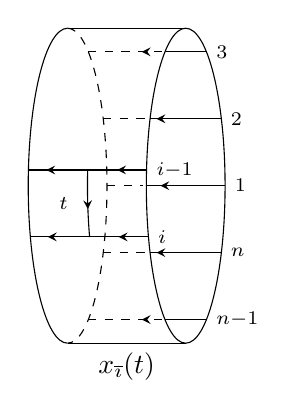
\begin{tikzpicture}
  \node[below] at (0,-2) {$x_{\ol{\imath}}(t)$};
  \draw (0.75,0) ellipse (0.5 and 2);
  %\draw (-1,0) ellipse (0.5 and 1);
  \draw (-0.75,2) arc (90:270:0.5 and 2);
  \draw[dashed] (-0.75,2) arc (90:-90:0.5 and 2);
  \draw[-] (0.75,2) -- (-0.75,2);
  \draw[-] (0.75,-2) -- (-0.75,-2);
  \draw[-] (1.25,0) -- (0.25,0);
  \draw[dashed] (-0.25,0) -- (0.21,0);
  \draw[singlearrow] (1.25,0) -- (-0.25,0);
  \node[right] at (1.25,0) {$\scriptstyle 1$};
  \draw[-] (1.2,-0.85) -- (0.3,-0.85);
  \draw[dashed] (-0.3,-0.85) -- (0.3,-0.85);
  \draw[singlearrow] (1.2,-0.85) -- (-0.3,-0.85);
  \node[right] at (1.2,-0.85) {$\scriptstyle n$};
  \draw[-] (1.015,-1.7) -- (0.49,-1.7);
  \draw[dashed] (-0.49,-1.7) -- (0.45,-1.7);
  \draw[singlearrow] (1.015,-1.7) -- (-0.49,-1.7);
  \node[right] at (1.015,-1.7) {$\scriptstyle n-1$};
  \draw[-] (-1.225,-0.65) -- (0.275,-0.65);
  \draw[doublearrow,draw] (0.275,-0.65) -- (-1.225,-0.65);
  \node[right] at (0.275,-0.65) {$\scriptstyle i$};
  %\draw[postaction=decorate] (-0.475,-0.65) arc (199:174.2:0.5 and 2);
  %\node at (-0.075,0.325) {$\scriptstyle u_i$};
  %\node at (-0.85,-0.875) {$\scriptstyle u_i^{-1}$};
  \draw[-] (-1.245,0.2) -- (0.255,0.2);
  \draw[doublearrow,draw] (0.255,0.2) -- (-1.245,0.2);
  \node[right] at (0.255,0.2) {$\scriptstyle i-1$};
  \draw[singlearrow,draw] (-0.495,0.2) arc (174.2:199:0.5 and 2);
  \node at (-0.8,-0.225) {$\scriptstyle t$};
  %\draw[-] (-1.18,1.05) -- (0.32,1.05);
  %\node[right] at (0.32,1.05) {$\scriptstyle i-1$};
  \draw[-] (1.015,1.7) -- (0.49,1.7);
  \draw[dashed] (-0.49,1.7) -- (0.45,1.7);
  \draw[singlearrow] (1.015,1.7) -- (-0.49,1.7);
  \node[right] at (1.015,1.7) {$\scriptstyle 3$};
  \draw[-] (1.2,0.85) -- (0.3,0.85);
  \draw[dashed] (-0.3,0.85) -- (0.3,0.85);
  \draw[singlearrow] (1.2,0.85) -- (-0.3,0.85);
  \node[right] at (1.2,0.85) {$\scriptstyle 2$};
\end{tikzpicture}
\quad\quad
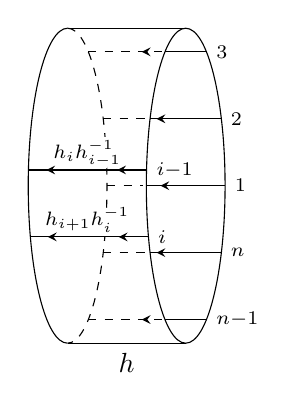
\begin{tikzpicture}
  \node[below,color=white] at (0,-2) {$()$};
  \node[below] at (0,-2) {$h$};
  \draw (0.75,0) ellipse (0.5 and 2);
  %\draw (-1,0) ellipse (0.5 and 1);
  \draw (-0.75,2) arc (90:270:0.5 and 2);
  \draw[dashed] (-0.75,2) arc (90:-90:0.5 and 2);
  \draw[-] (0.75,2) -- (-0.75,2);
  \draw[-] (0.75,-2) -- (-0.75,-2);
  \draw[-] (1.25,0) -- (0.25,0);
  \draw[dashed] (-0.25,0) -- (0.21,0);
  \draw[singlearrow] (1.25,0) -- (-0.25,0);
  \node[right] at (1.25,0) {$\scriptstyle 1$};
  \draw[-] (1.2,-0.85) -- (0.3,-0.85);
  \draw[dashed] (-0.3,-0.85) -- (0.3,-0.85);
  \draw[singlearrow] (1.2,-0.85) -- (-0.3,-0.85);
  \node[right] at (1.2,-0.85) {$\scriptstyle n$};
  \draw[-] (1.015,-1.7) -- (0.49,-1.7);
  \draw[dashed] (-0.49,-1.7) -- (0.45,-1.7);
  \draw[singlearrow] (1.015,-1.7) -- (-0.49,-1.7);
  \node[right] at (1.015,-1.7) {$\scriptstyle n-1$};
  \draw[-] (-1.225,-0.65) -- (0.275,-0.65);
  \draw[doublearrow] (0.275,-0.65) -- (-1.225,-0.65);
  \node[right] at (0.275,-0.65) {$\scriptstyle i$};
  \draw[thick,color=white] (-0.255,-0.28) arc (-8:-18.5:0.5 and 2);
  \node at (-0.5,-0.435) {$\scriptstyle h_{i+1}h_i^{-1}$};
  %\draw[postaction=decorate] (-0.475,-0.65) arc (199:174.2:0.5 and 2);
  \draw[-] (-1.245,0.2) -- (0.255,0.2);
  \draw[doublearrow] (0.255,0.2) -- (-1.245,0.2);
  \node[right] at (0.255,0.2) {$\scriptstyle i-1$};
  \draw[thick,color=white] (-0.255,0.22) arc (6.25:18:0.5 and 2);
  \node at (-0.5,0.405) {$\scriptstyle h_ih_{i-1}^{-1}$};
  %\draw[postaction=decorate] (-0.495,0.2) arc (174.2:199:0.5 and 2);
  %\node at (-0.8,-0.225) {$\scriptstyle t_{-i}$};
  %\draw[-] (-1.18,1.05) -- (0.32,1.05);
  %\node[right] at (0.32,1.05) {$\scriptstyle i-1$};
  \draw[-] (1.015,1.7) -- (0.49,1.7);
  \draw[dashed] (-0.49,1.7) -- (0.45,1.7);
  \draw[singlearrow] (1.015,1.7) -- (-0.49,1.7);
  \node[right] at (1.015,1.7) {$\scriptstyle 3$};
  \draw[-] (1.2,0.85) -- (0.3,0.85);
  \draw[dashed] (-0.3,0.85) -- (0.3,0.85);
  \draw[singlearrow] (1.2,0.85) -- (-0.3,0.85);
  \node[right] at (1.2,0.85) {$\scriptstyle 2$};
\end{tikzpicture}
\quad\quad
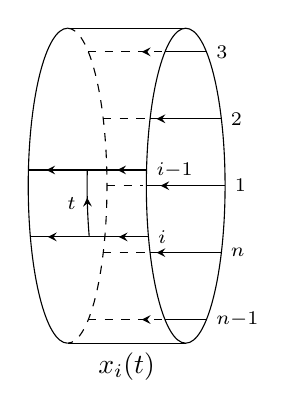
\begin{tikzpicture}
  \node[below] at (0,-2) {$x_i(t)$};
  \draw (0.75,0) ellipse (0.5 and 2);
  %\draw (-1,0) ellipse (0.5 and 1);
  \draw (-0.75,2) arc (90:270:0.5 and 2);
  \draw[dashed] (-0.75,2) arc (90:-90:0.5 and 2);
  \draw[-] (0.75,2) -- (-0.75,2);
  \draw[-] (0.75,-2) -- (-0.75,-2);
  \draw[-] (1.25,0) -- (0.25,0);
  \draw[dashed] (-0.25,0) -- (0.21,0);
  \draw[singlearrow] (1.25,0) -- (-0.25,0);
  \node[right] at (1.25,0) {$\scriptstyle 1$};
  \draw[-] (1.2,-0.85) -- (0.3,-0.85);
  \draw[dashed] (-0.3,-0.85) -- (0.3,-0.85);
  \draw[singlearrow] (1.2,-0.85) -- (-0.3,-0.85);
  \node[right] at (1.2,-0.85) {$\scriptstyle n$};
  \draw[-] (1.015,-1.7) -- (0.49,-1.7);
  \draw[dashed] (-0.49,-1.7) -- (0.45,-1.7);
  \draw[singlearrow] (1.015,-1.7) -- (-0.49,-1.7);
  \node[right] at (1.015,-1.7) {$\scriptstyle n-1$};
  \draw[-] (-1.225,-0.65) -- (0.275,-0.65);
  \draw[doublearrow,draw] (0.275,-0.65) -- (-1.225,-0.65);
  \node[right] at (0.275,-0.65) {$\scriptstyle i$};
  \draw[singlearrow,draw] (-0.475,-0.65) arc (199:174.2:0.5 and 2);
  \node at (-0.7,-0.225) {$\scriptstyle t$};
  \draw[-] (-1.245,0.2) -- (0.255,0.2);
  \draw[doublearrow,draw] (0.255,0.2) -- (-1.245,0.2);
  \node[right] at (0.255,0.2) {$\scriptstyle i-1$};
  %\draw[postaction=decorate] (-0.495,0.2) arc (174.2:199:0.5 and 2);
  %\draw[-] (-1.18,1.05) -- (0.32,1.05);
  %\node[right] at (0.32,1.05) {$\scriptstyle i-1$};
  \draw[-] (1.015,1.7) -- (0.49,1.7);
  \draw[dashed] (-0.49,1.7) -- (0.45,1.7);
  \draw[singlearrow] (1.015,1.7) -- (-0.49,1.7);
  \node[right] at (1.015,1.7) {$\scriptstyle 3$};
  \draw[-] (1.2,0.85) -- (0.3,0.85);
  \draw[dashed] (-0.3,0.85) -- (0.3,0.85);
  \draw[singlearrow] (1.2,0.85) -- (-0.3,0.85);
  \node[right] at (1.2,0.85) {$\scriptstyle 2$};
\end{tikzpicture}
\caption{The constituent networks used to define $\cN^{u,v}$.}\label{fig:networks on cylinders}
\end{figure}


\begin{definition}\label{def:network}
Let $u$, $v$ be elements of the Weyl group of $\widetilde{LSL}_n$ together with a choice of reduced words $u=s_{i_1}\cdots s_{i_{\ell(u)}}$, $v=s_{j_1}\cdots s_{j_{\ell(v)}}$. We associate to this data a weighted directed network $\cN^{u,v}$ on a cylinder, by abuse omitting the choice of reduced words from the notation. The edge weights of the network will take values in the Laurent polynomial ring
\[
\kk[t_{1}^{\pm1},\dotsc,t_{\ell(v)}^{\pm 1},h_1^{\pm 1},\dotsc,h_{n}^{\pm 1},t_{\ol{1}}^{\pm 1},\dotsc,t_{\ol{\ell(u)}}^{\pm 1}].
\] 
We declare one boundary component of the cylinder to be incoming and the other outgoing, and begin by associating a smaller cylindrical network to each factor in Equation~\ref{eq:uvfactorization} (see Figure~\ref{fig:networks on cylinders}). 

For $1 \leq i \leq n$, the networks associated to $x_i(t)$ and $x_{\ol{\imath}}(t)$ contain $n$ horizontal \newword{levels} running from the incoming boundary to the outgoing boundary. These are labelled by $\ZZ_n$ compatibly with their cyclic ordering and all have weight $1$. There is also a vertical \newword{bridge} having weight $t$ running between the $(i-1)^{st}$ level and the $i^{th}$ level; for $x_i(t)$ this bridge is oriented from the $(i-1)^{st}$ level to the $i^{th}$ level, while for $x_{\ol{\imath}}(t)$ this bridge is oriented from the $i^{th}$ level to the $(i-1)^{st}$.

%For $i\in[-n,-1]\cup[1,n]$ define a directed network on a cylinder (which we associate with $x_i(t_i)$) containing $n$ pairwise disjoint \emph{horizontal} edges of weight $1$ running from the right-hand boundary component to the left-hand boundary component, which are labelled by $\ZZ_n$ compatibly with their cyclic ordering, and a (\emph{vertical}) \emph{bridge} of weight $t_i$ joining the $(i-1)^{st}$\sayHW{wrong if $i < 0$?}\sayDR{Ugh, signs...I guess it should have an absolute value $|i|$ but this will be really ugly.} horizontal edge and the $i^{th}$ horizontal edge, which is oriented upward for $i>0$ and downward for $i<0$ (see Figure~\ref{fig:networks on cylinders}).  

The network associated to the Cartan factor $h$ again has $n$ horizontal levels running from the incoming boundary to the outgoing boundary and labelled by $\ZZ_n$. The $i^{th}$ level is of weight $h_{i+1}h_{i}^{-1}$. 

The network $\cN^{u,v}$ is now defined by gluing these constituent networks together in the order they appear in Equation~\ref{eq:uvfactorization} (see Figure~\ref{fig:totalnetwork}). Given two adjacent factors, the incoming boundary of the left is glued to the outgoing boundary of the right so that the horizontal levels of each are aligned. 
%For $i\in[1,n]$ define another directed network on a cylinder (which we associate with $h_i^{\alpha_i^\vee}$) again containing the $n$ pairwise disjoint horizontal edges with the $i^{th}$ horizontal edge of weight $h_i^{-1}$, the $(i-1)^{st}$ horizontal edge of weight $h_i$, and all other horizontal edges of weight 1 (see Figure~\ref{fig:networks on cylinders}).
%\bigskip
%Given reduced decompositions $u=s_{\sigma_1}\cdots s_{\sigma_{\ell(u)}}$ and $v=s_{\tau_1}\cdots s_{\tau_{\ell(v)}}$, define the network $\cN^{u,v}$ to be the concatenation of the basic networks associated to the factors in the decomposition 
%\begin{equation}\label{eq:double Bruhat generic element}
%  g=x_{-\tau_{\ell(v)}}(t_{-\tau_{\ell(v)}})\cdots x_{-\tau_1}(t_{-\tau_1}) hx_{\sigma_{\ell(u)}}(t_{\sigma_{\ell(u)}}) \cdots x_{\sigma_1}(t_{\sigma_1})
%\end{equation}\sayDR{Check whether order of factors is correct.}
%of a generic element of $G^{u,v}$, where $h$ factors as $\prod\limits_{i=1}^n h_i$ with $h_i=\big(h^{\omega_i}\big)^{\alpha_i^\vee}$.
%It follows that $h_i^{\omega_i}=h^{\omega_i}$ and $h_i^{\omega_j}=1$ for $i\ne j$.  
%Here we abuse notation slightly and write $h_i$ also for the value $h_i^{\omega_i}$.
%Given a Coxeter element $c = s_{\sigma_1} \dotsc s_{\sigma_n}$, define the \emph{network} $\cN_c$ to be the concatenation of the basic networks above associated to the factors in the decomposition 
%\[g=x_{-\sigma_1}(t_{-\sigma_1})\cdots x_{-\sigma_n}(t_{-\sigma_n}) hx_{\sigma_n}(t_{\sigma_n}) \cdots x_{\sigma_1}(t_{\sigma_1})\]
%of a generic element of $G^{c,c^{-1}}$, where $h$ factors as $\prod\limits_{i=1}^n h_i$ with $h_i=\big(h^{\omega_i}\big)^{\alpha_i^\vee}$.
%It follows that $h_i^{\omega_i}=h^{\omega_i}$ and $h_i^{\omega_j}=1$ for $i\ne j$.  
%Here we abuse notation slightly and write $h_i$ also for the value $h_i^{\omega_i}$.
\end{definition}

\begin{figure}
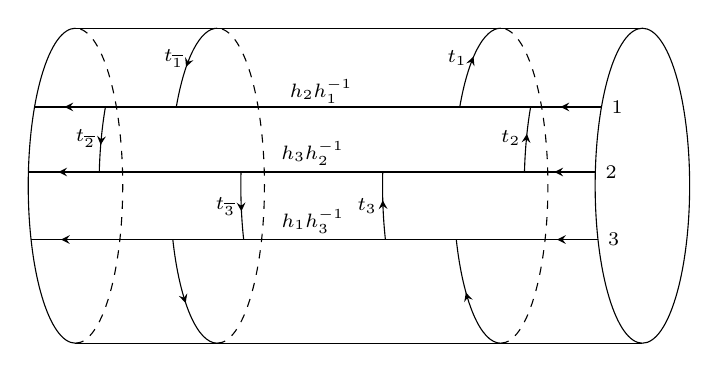
\begin{tikzpicture}
  % drawing parameters
  \pgfmathsetmacro{\ehgt}{2} % vertical radius of ellipse
  \pgfmathsetmacro{\edpt}{0.6} % horizontal radius of ellipse
  \pgfmathsetmacro{\ewdt}{0.9} % horizontal distance in between slices
  \pgfmathsetmacro{\fang}{150} % angle of topmost horizontal line
  \pgfmathsetmacro{\ang}{25} % angle in between horizontal lines
  \pgfmathsetmacro{\ask}{-7} % angle distance of labels
  \pgfmathsetmacro{\hsk}{-0.2} %horizontal distance of labels

  % left side
  \draw ([shift={(90:{\edpt} and \ehgt)}]0,0) arc (90:270:{\edpt} and \ehgt);
  \draw [dashed] ([shift={(-90:{\edpt} and \ehgt)}]0,0) arc (-90:90:{\edpt} and \ehgt);

  % first block
  \draw [singlearrow,draw] ([shift={(\fang:{\edpt} and \ehgt)}]\ewdt,0) arc (\fang:\fang+\ang:{\edpt} and \ehgt);
  \node at ([shift={(\fang+0.5*\ang:{\edpt} and \ehgt)}]\ewdt+\hsk,0) {$\scriptstyle t_{\ol{2}}$};
  
  % second block
  \draw [singlearrow,draw] ([shift={(90:{\edpt} and \ehgt)}]2*\ewdt,0) arc (90:\fang:{\edpt} and \ehgt);
  \draw [dashed] ([shift={(-90:{\edpt} and \ehgt)}]2*\ewdt,0) arc (-90:90:{\edpt} and \ehgt);
  \draw [singlearrow,draw] ([shift={(\fang+2*\ang:{\edpt} and \ehgt)}]2*\ewdt,0) arc (\fang+2*\ang:270:{\edpt} and \ehgt);
  \node at ([shift={({0.6*(\fang-90)+90}:{\edpt} and \ehgt)}]2*\ewdt+\hsk,0) {$\scriptstyle t_{\ol{1}}$};

  % third block
  \draw [singlearrow,draw] ([shift={(\fang+\ang:{\edpt} and \ehgt)}]3*\ewdt,0) arc (\fang+\ang:\fang+2*\ang:{\edpt} and \ehgt);
  \node at ([shift={(\fang+1.5*\ang:{\edpt} and \ehgt)}]3*\ewdt+\hsk,0) {$\scriptstyle t_{\ol{3}}$};
  
  % fourth block
  \draw ([shift={(\fang:{\edpt} and \ehgt)}]0,0) -- ([shift={(150:{\edpt} and \ehgt)}]8*\ewdt,0);
  \draw [singlearrowreversed] ([shift={(\fang:{\edpt} and \ehgt)}]0,0) -- ([shift={(150:{\edpt} and \ehgt)}]\ewdt,0);
  \draw [singlearrowreversed] ([shift={(\fang:{\edpt} and \ehgt)}]7*\ewdt,0) -- ([shift={(150:{\edpt} and \ehgt)}]8*\ewdt,0);
  \node at ([shift={(\fang+\ask:{\edpt} and \ehgt)}]4*\ewdt,0) {$\scriptstyle h_2h_1^{-1}$};

  \draw ([shift={(\fang+\ang:{\edpt} and \ehgt)}]0,0) -- ([shift={(\fang+\ang:{\edpt} and \ehgt)}]8*\ewdt,0);
  \draw [singlearrowreversed] ([shift={(\fang+\ang:{\edpt} and \ehgt)}]0,0) -- ([shift={(\fang+\ang:{\edpt} and \ehgt)}]\ewdt,0);
  \draw [singlearrowreversed] ([shift={(\fang+\ang:{\edpt} and \ehgt)}]7*\ewdt,0) -- ([shift={(\fang+\ang:{\edpt} and \ehgt)}]8*\ewdt,0);
  \node at ([shift={(\fang+\ask+\ang:{\edpt} and \ehgt)}]4*\ewdt,0) {$\scriptstyle h_3h_2^{-1}$};

  \draw ([shift={(\fang+2*\ang:{\edpt} and \ehgt)}]0,0) -- ([shift={(\fang+2*\ang:{\edpt} and \ehgt)}]8*\ewdt,0);
  \draw [singlearrowreversed] ([shift={(\fang+2*\ang:{\edpt} and \ehgt)}]0,0) -- ([shift={(\fang+2*\ang:{\edpt} and \ehgt)}]\ewdt,0);
  \draw [singlearrowreversed] ([shift={(\fang+2*\ang:{\edpt} and \ehgt)}]7*\ewdt,0) -- ([shift={(\fang+2*\ang:{\edpt} and \ehgt)}]8*\ewdt,0);
  \node at ([shift={(\fang+\ask+2*\ang:{\edpt} and \ehgt)}]4*\ewdt,0) {$\scriptstyle h_1h_3^{-1}$};

  % fifth block
  \draw [singlearrowreversed,draw] ([shift={(\fang+\ang:{\edpt} and \ehgt)}]5*\ewdt,0) arc (\fang+\ang:\fang+2*\ang:{\edpt} and \ehgt);
  \node at ([shift={(\fang+1.5*\ang:{\edpt} and \ehgt)}]5*\ewdt+\hsk,0) {$\scriptstyle t_{3}$};
  
  % sixth block
  \draw [singlearrowreversed,draw] ([shift={(90:{\edpt} and \ehgt)}]6*\ewdt,0) arc (90:\fang:{\edpt} and \ehgt);
  \draw [dashed] ([shift={(-90:{\edpt} and \ehgt)}]6*\ewdt,0) arc (-90:90:{\edpt} and \ehgt);
  \draw [singlearrowreversed,draw] ([shift={(\fang+2*\ang:{\edpt} and \ehgt)}]6*\ewdt,0) arc (\fang+2*\ang:270:{\edpt} and \ehgt);
  \node at ([shift={({0.6*(\fang-90)+90}:{\edpt} and \ehgt)}]6*\ewdt+\hsk,0) {$\scriptstyle t_{1}$};

  % seventh block
  \draw [singlearrowreversed,draw] ([shift={(\fang:{\edpt} and \ehgt)}]7*\ewdt,0) arc (\fang:\fang+\ang:{\edpt} and \ehgt);
  \node at ([shift={(\fang+0.5*\ang:{\edpt} and \ehgt)}]7*\ewdt+\hsk,0) {$\scriptstyle t_{2}$};

  % right side
  \draw (8*\ewdt,0) ellipse ({\edpt} and \ehgt);
  \node at ([shift={(\fang:{\edpt} and \ehgt)}]8*\ewdt-\hsk,0) {$\scriptstyle 1$};
  \node at ([shift={(\fang+\ang:{\edpt} and \ehgt)}]8*\ewdt-\hsk,0) {$\scriptstyle 2$};
  \node at ([shift={(\fang+2*\ang:{\edpt} and \ehgt)}]8*\ewdt-\hsk,0) {$\scriptstyle 3$};

  % top and bottom
  \draw ([shift={(90:{\edpt} and \ehgt)}]0,0) -- ([shift={(90:{\edpt} and \ehgt)}]8*\ewdt,0);
  \draw ([shift={(-90:{\edpt} and \ehgt)}]0,0) -- ([shift={(-90:{\edpt} and \ehgt)}]8*\ewdt,0);
\end{tikzpicture}
\caption{The network $\cN^{c,c^{-1}}$ for $c = s_2 s_1 s_3$. It encodes the factorization of a generic element of $\widetilde{LSL}_3^{c,c^{-1}}$ as $g = x_{\ol{2}}(t_{\ol{2}})x_{\ol{1}}(t_{\ol{1}})x_{\ol{3}}(t_{\ol{3}})hx_{3}(t_{3})x_{1}(t_{1})x_{2}(t_{2})$.}
\label{fig:totalnetwork}
\end{figure}

By a \newword{path} in $\cN^{u,v}$ we always mean a path which begins at an incoming boundary vertex, is directed compatibly with the edges of $\cN^{u,v}$, and ends at an outgoing boundary vertex. 
% directed path in the network which begins at a source on the right-hand side of the cylinder, is directed compatibly with the edges of $\cN^{u,v}$, and ends at a sink on the left-hand side of the cylinder. 
If $P = \{P_i\}$ is a collection of paths, we write $\partial_{in}P \subset \ZZ_n$ for the set of incoming boundary vertices at which paths in $P$ begin; $\partial_{out}P \subset \ZZ_n$ denotes the corresponding set of outgoing boundary vertices. 
The \newword{weight} of a path is the product of the weights of the edges it traverses, and the weight $wt(P)$ of a collection of paths is the product of the weights of its constituent paths.  

Given $S \subsetneq \ZZ_n$, let
\[ \omega_S = \sum_{i \in S} \omega_{i+1} - \omega_i \in P^\circ \subset \widehat{P}.\] 
Recall that $P^\circ$, the weight lattice of $SL_n$, is contained in the complement of both the Tits cone and its negative in $\widehat{P}$. The level zero representation $V(\omega_S)$ is $\big(\bigwedge^{|S|}\kk^{n-1}\big)[z^{\pm 1}]$ with its natural $\widetilde{LSL}_n$ action. Definition~\ref{def:network} is motivated by the following observation:

\begin{proposition}\label{prop:minorsfrompaths}
  Suppose $g\in G^{u,v}$ factors as %in Equation \ref{eq:uvfactorization}, 
\[
g = x_{\ol{\imath_1}}(t_{\ol{1}})\cdots x_{\ol{\imath_{\ell(u)}}}(t_{\ol{\ell(u)}})hx_{j_1}(t_{1}) \cdots x_{j_{\ell(v)}}(t_{\ell(v)})
\]
and let $h_i:= h^{\omega_i}$. Then \[ \Delta_{\omega_S}(g) = \sum_{P: S \to S} wt(P), \]
  where the sum is over collections $P$ of pairwise disjoint paths in $\cN^{u,v}$ with $\partial_{in}P = \partial_{out}P = S$.
\end{proposition}
\begin{proof}
  The representation $\big(\bigwedge^{|S|}\kk^{n-1}\big)[z^{\pm 1}]$ has a natural basis $\{ e_{j_1} \wedge \cdots \wedge e_{j_{|S|}} z^d\}$ labelled by pairs of an $|S|$-element subset of $\ZZ_n$ and an integer $d$. The networks associated to $x_i(t)$, $x_{\ol{\imath}}(t)$, and $h$ directly encode the action of the corresponding group elements in this basis (see [GSV, FM ??] for related constructions). If $S = \{i_1,\dotsc,i_{|S|}\}$, then by a generalized Lindstr\"om-Gessel-Viennot argument the sum over collections of nonintersecting paths with $\partial_{in}P = \partial_{out}P = S$ computes the diagonal matrix coefficient by which $g$ rescales the basis element $e_{i_1} \wedge \cdots \wedge e_{i_{|S|}}$. Since this element has weight $\omega_S$, this matrix coefficient is $\Delta_{\omega_S}(g)$. 
% (the exponent $d$ could be encoded more directly by pulling back $\cN^{u,v}$ to the universal cover of the cylinder -- this network would have infinitely many boundary vertices and basis elements are in bijection with certain $|S|$-element subsets of them
%  Write $r=|S|$.  
%  Inside the irreducible representation $\big(\!\bigwedge^{\!r}\CC^n\big)[z^{\pm 1}]$ of $G$, the vector $\bigwedge\limits_{i\in S} e_i$ (following Definition~\ref{def:minors} the choice of sign will be irrelevant) has weight $\omega_S$ and thus this representation identifies with $V(\omega_S)$.
%  By construction, each basic network $x_i(t_i)$ for $i\in[-n,-1]\cup[1,n]$ and $h_i$ for $i\in[1,n]$ encodes the action of the corresponding group element on the standard basis $\{ e_{j_1} \wedge \cdots \wedge e_{j_r} z^d\}$ of $\big(\!\bigwedge^{\!r}\CC^n\big)[z^{\pm 1}]$ labelled by pairs of an $r$-element subset of $\ZZ_n$ and an integer $d$.  Thus the network $\cN^{u,v}$ encodes the action of a generic element $g\in G^{c,c^{-1}}$ given by \eqref{eq:double Bruhat generic element} on this basis and the result then follows from the definition of $\Delta_{\omega_S}$.
\end{proof}

We now return to the specific case of $\widetilde{LSL}_n^{c,c^{-1}}$, where $c = s_{\sigma_1}\cdots s_{\sigma_{n}}$ is a fixed Coxeter element. From now on we reindex the factorization of Equation~\ref{eq:uvfactorization} in a way tailored to this case:
\begin{equation}
\label{eq:coxfactorization}
g = x_{\ol{\sigma_1}}(t_{\ol{\sigma_1}}) \cdots x_{\ol{\sigma_n}}(t_{\ol{\sigma_n}})h x_{\sigma_n}(t_{\sigma_n}) \cdots x_{\sigma_1}(t_{\sigma_1}).
\end{equation}
To use the preceding proposition effectively, we collect some elementary combinatorial observations about collections of pairwise disjoint paths $P$ in $\cN^{c,c^{-1}}$. 
Note that when $u$ and $v$ are Coxeter elements the choice of reduced word in Definition~\ref{def:network} is immaterial: different reduced words differ by relations of the form $s_i s_j = s_j s_i$ for $a_{ij} = 0$, and these relations do not change the combinatorics of the network. 
Given a collection $P$ of disjoint paths, define its \newword{bridge set} $\beta(P)\subset\ZZ_n$ by letting $j\in\beta(P)$ if and only if a path in $P$ traverses the unique bridge of weight $t_j$.


\begin{lemma}\label{lem:phi}
  Let $P$ be a collection of pairwise disjoint paths in $\cN^{c,c^{-1}}$.  Then:
  \begin{enumerate}
    \item for $j\in\partial_{in}P$, $j+1\in\beta(P)$ implies $j+1\to j$ in $Q$ and $j\in\beta(P)$;
    \item for $j\notin\partial_{in}P$, $j\in\beta(P)$ implies $j\to j+1$ in $Q$ and $j+1\in\beta(P)$.
  \end{enumerate}
\end{lemma}
\begin{proof}
If $c = s_{\sigma_1}\cdots s_{\sigma_{n}}$, then by our definitions $(\sigma_1,\ldots,\sigma_{n})$ is sink adapted for $Q$. The orientation of the arrow connecting vertices $j$ and $j+1$ is thus related to the local structure of the network $\cN^{c,c^{-1}}$ as in Figure~\ref{fig:quivernetwork}. The result follows immediately by comparing the statements against the picture.
\end{proof} 

\begin{figure}
  \begin{center}
  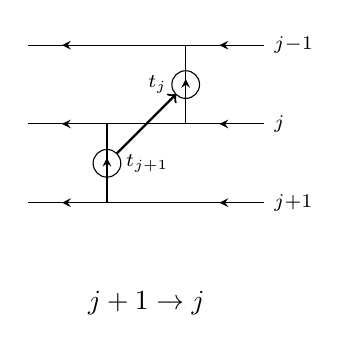
\begin{tikzpicture}
    \node[below] at (0,-2) {$j+1\to j$};
    \draw[singlearrow,draw] (1.5,1) -- (0.5,1);
    \draw[-] (0.5,1) -- (-0.5,1);
    \draw[singlearrow,draw] (-0.5,1) -- (-1.5,1);
    \node[right] at (1.5,1) {$\scriptstyle j-1$};
    \draw[singlearrow,draw] (0.5,0) -- (0.5,1);
    \node[left] at (0.5,0.5) {$\scriptstyle t_j\ $};
    \draw[singlearrow,draw] (1.5,0) -- (0.5,0);
    \draw[-] (0.5,0) -- (-0.5,0);
    \draw[singlearrow,draw] (-0.5,0) -- (-1.5,0);
    \node[right] at (1.5,0) {$\scriptstyle j$};
    \draw[singlearrow,draw] (-0.5,-1) -- (-0.5,0);
    \node[right] at (-0.5,-0.5) {$\ \scriptstyle t_{j+1}$};
    \draw[singlearrow,draw] (1.5,-1) -- (0.5,-1);
    \draw[-] (0.5,-1) -- (-0.5,-1);
    \draw[singlearrow,draw] (-0.5,-1) -- (-1.5,-1);
    \node[right] at (1.5,-1) {$\scriptstyle j+1$};
    \draw (-0.5,-0.5) circle (5pt);
    \draw (0.5,0.5) circle (5pt);
    \draw[thick,->] (-0.38,-0.38) -- (0.38,0.38);
  \end{tikzpicture}
  \qquad\qquad
  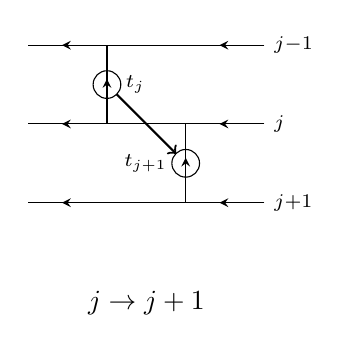
\begin{tikzpicture}
    \node[below] at (0,-2) {$j\to j+1$};
    \draw[singlearrow,draw] (1.5,1) -- (0.5,1);
    \draw[-] (0.5,1) -- (-0.5,1);
    \draw[singlearrow,draw] (-0.5,1) -- (-1.5,1);
    \node[right] at (1.5,1) {$\scriptstyle j-1$};
    \draw[singlearrow,draw] (-0.5,0) -- (-0.5,1);
    \node[right] at (-0.5,0.5) {$\ \scriptstyle t_j$};
    \draw[singlearrow,draw] (1.5,0) -- (0.5,0);
    \draw[-] (0.5,0) -- (-0.5,0);
    \draw[singlearrow,draw] (-0.5,0) -- (-1.5,0);
    \node[right] at (1.5,0) {$\scriptstyle j$};
    \draw[singlearrow,draw] (0.5,-1) -- (0.5,0);
    \node[left] at (0.5,-0.5) {$\scriptstyle t_{j+1}\ $};
    \draw[singlearrow,draw] (1.5,-1) -- (0.5,-1);
    \draw[-] (0.5,-1) -- (-0.5,-1);
    \draw[singlearrow,draw] (-0.5,-1) -- (-1.5,-1);
    \node[right] at (1.5,-1) {$\scriptstyle j+1$};
    \draw (-0.5,0.5) circle (5pt);
    \draw (0.5,-0.5) circle (5pt);
    \draw[thick,->] (-0.38,0.38) -- (0.38,-0.38);
  \end{tikzpicture}
  \end{center}
\caption{
The local picture relating the network $\cN^{c,c^{-1}}$ to the orientation of the arrow of $Q$ connecting vertices $j$ and $j+1$, where we draw the vertices on top of the corresponding bridges in $\cN^{c,c^{-1}}$}\label{fig:quivernetwork}
\end{figure}
  
%\begin{corollary}
%  Let $P$ be a collection of pairwise disjoint paths in $\cN^{c,c^{-1}}$.  Then:
%  \begin{enumerate}
%    \item If $i \to i+1$ in $Q$, $i \in \beta(P)$, and $i \notin \partial_{in}(P)$, then $i + 1 \in \beta(P)$.
%    \item If $i \to i+1$ in $Q$ and $i \in \partial_{in}P$, then $i +1 \notin \beta(P)$.
%    \item If $i+1 \to i$ in $Q$, $i \in \partial_{in}P$, and $i+1 \in \beta(P)$, then $i \in \beta(P)$.
%    \item If $i \notin \beta(P)$ and $i \in \partial_{in}P$, then $i +1 \notin \beta(P)$.
%  \end{enumerate}
%\end{corollary}

We now turn to the main result of the section.  We will freely use the isomorphism $\cA_{\Qdp} \cong \kk[\widetilde{LSL}_n^{c,c^{-1}}]$ to identify elements of $\cA_{\Qdp}$ with elements of 
\[
\kk[t_{1}^{\pm1},\dotsc,t_{n}^{\pm 1},h_1^{\pm 1},\dotsc,h_{n}^{\pm 1},t_{\ol{1}}^{\pm 1},\dotsc,t_{\ol{n}}^{\pm 1}]
\]
by evaluating them on a generic $g \in \widetilde{LSL}_n^{c,c^{-1}}$ factored as in Equation~\ref{eq:coxfactorization} (and setting $h_i := h^{\omega_i}$). For example, we have 
\begin{equation}\label{eq:typeAyhat}
x_i = h_i,\quad\quad \hat{y}_i = t_it_{\ol{\imath}}h_{i-1}^{-1}h_i^2h_{i+1}^{-1},
\end{equation}
the latter following by reindexing vertices of $Q$ in the results of Lemma~\ref{lemma:coefficients_values} with the present conventions, then plugging them into the definition of $\hat{y}_i$.

\begin{theorem}\label{th:cluster character equals minor}
Let $\Qrep_{[k,\ell]}$ be a rigid regular representation of $Q$. Then in $\cA_{\Qdp} \cong \kk[\widetilde{LSL}_n^{c,c^{-1}}]$ the regular cluster variable $x_{\Qrep_{[k,\ell]}}$ is the restriction of the level zero minor $\Delta_{\bfg(\Qrep_{[k,\ell]})}$. 
%Then the isomorphism $\cA_{\Qdp} \cong \kk[\widetilde{LSL}_n^{c,c^{-1}}]$ of Theorem~\ref{thm:coordring} identifies the regular cluster variable $x_{\Qrep_{[k,\ell]}}$ with the restriction of the level zero minor $\Delta_{\omega_{S_{[k,\ell]}}}$. 
\end{theorem}
\begin{proof}
Recall from Lemma~\ref{lem:regulargvectors} the subset $S_{[k,\ell]} \subset \ZZ_n$ such that $\bfg(\Qrep_{[k,\ell]}) = \omega_{S_{[k,\ell]}}$. 
Let $\cP_{[k,\ell]}$ denote the set of pairwise disjoint collections of paths in $\cN^{c,c^{-1}}$ with $\partial_{in}P = \partial_{out}P = S_{[k,\ell]}$. 
%Our goal is to identify this with the evaluation $x_{\Qrep_{[k,\ell]}}(g)$ of the cluster character from \eqref{eq:regular cluster characters}, where the functions $x_i,\hat y_j\in\kk[G^{c,c^{-1}}]$ are determined by the initial cluster \eqref{eq:initialcluster}.\sayDR{Say this better, maybe compute $x_i(g)$ and $\hat y_j(g)$ here?  I just realized an abuse of notation by writing $x_i$ in both sections 2.2 and 2.3.}
%As in Lemma \ref{lem:phi}, we define the bridge set $\beta(P) \subset \ZZ_n$ by letting $j \in \beta(P)$ if and only if a path in $P$ traverses the unique edge of weight $t_j$. 
We claim that for $P \in \cP_{[k,\ell]}$: 
\begin{enumerate}[\quad\upshape (a)]
\item the bridge set $\beta(P)$ is a target-closed subset of $[k,\ell]$, 
\item we have
\[
wt(P) = x^{\bfg(\Qrep_{[k,\ell]})} \prod_{j \in \beta(P)} \hat{y}_j,
\]
\item 
the assignment $P \mapsto \beta(P)$ defines a bijection between $\cP_{[k,\ell]}$ and the set $\cE_{[k,\ell]}$ of target-closed subsets of $[k,\ell]$.
\end{enumerate}
The main claim follows from these given Propositions~\ref{prop:regular coindices} and~\ref{prop:minorsfrompaths}.

%By Proposition \ref{prop:minorsfrompaths}, given a generic $g \in \widetilde{LSL}_n^{c,c^{-1}}$ factored as in Equation \ref{eq:coxfactorization}, we have  
%\[
%\Delta_{\omega_{S_{[k,\ell]}}}(g) = \sum_{P: S_{[k,\ell]} \to S_{[k,\ell]}} wt(P),
%\]
%where the sum is over collections $P$ of pairwise disjoint paths in $\cN^{u,v}$ with $\partial_{in}P = \partial_{out}P = S_{[k,\ell]}$. Let $\cP_{[k,\ell]}$ denote the set of such collections. 


As in Proposition~\ref{prop:regular coindices}, we let $i_1 < \cdots < i_m$ and $o_1 < \cdots < o_m$ denote the labels of the sinks and sources of $Q$ contained in $[k,\ell]$.  
We consider the case where the first source in $[k,\ell]$ comes before the first sink (i.e. $o_1 < i_1$ in $[k,\ell]$), the opposite case following by a symmetric argument.%\sayDR{Thinking of cluster variables in terms of the opposite quiver dualizes representations, negates $g$-vectors, and negates the principal part of $\tilde B$ (this in effect interchanges $h_i$ with $h_i^{-1}$).  Applying $\iota$ to $g$ has the same effect.}\sayHW{If we day ``by symmetry'' then we should write this out - I'm currently too lazy to do this, hence changing to the less slick statement that ``proving the other case has the same flavor.''} 
Recall that in this case
\[S_{[k,\ell]} = [k,o_1-1] \cup [i_1,o_2-1] \cup \cdots \cup [i_m,\ell].\]

Let $P \in \cP_{[k,\ell]}$.  Since $o_1<i_1$, we have $j+1\to j$ in $Q$ for each $j\in[k^-,k-1]$, where $k^-$ is the nearest sink less that $k$ (i.e. none of $[k^-+1,k]$ is a sink).  
But $[k^-,k-1]\cap\partial_{in}P=\emptyset$ and thus part (2) of Lemma~\ref{lem:phi} implies $j\notin\beta(P)$ for any $j\in[k^-,k-1]$.  
Similarly, $o_m<i_m$ gives $j\to j-1$ in $Q$ for each $j\in[\ell+1,\ell^+]$, where $\ell^+$ is the nearest source after $\ell$.  
Applying part (2) of Lemma~\ref{lem:phi} inductively beginning with the source $j=\ell^+$, we see that $j\notin\beta(P)$ for any $j\in[\ell+1,\ell^+]$.  
Noting that $[\ell^+,k^-]\cap\partial_{in}P=\emptyset$ and then arguing as above we conclude that $\beta(P)\subset[k,\ell]$.

Write $i_0=k$ and $i_{m+1}=o_{m+1}=\ell+1$.  For $1\le r\le m+1$ and $j\in[i_{r-1},o_r-1]\subset\partial_{in}P$, we have $j+1\to j$ in $Q$ and part (1) of Lemma~\ref{lem:phi} says $j+1\in\beta(P)$ implies $j\in\beta(P)$.  
For $1\le r\le m$ and $j\in[o_r,i_r-1]$, we have $j\notin\partial_{in}P$ and $j\to j+1$ in $Q$ so that part (2) of Lemma~\ref{lem:phi} says $j\in\beta(P)$ implies $j+1\in\beta(P)$.  
Putting these observations together, we conclude that $\beta(P)\subset[k,\ell]$ is target-closed and (a) is established.

Now suppose $E\in\cE_{[k,\ell]}$ is a target-closed subset of $[k,\ell]$.  
Write $P_0\in\cP_{[k,\ell]}$ for the trivial collection of pairwise disjoint paths in which the path beginning on level $j\in S_{[k,\ell]}=\partial_{in}P_0$ stays on level $j$ without traversing any bridges. 
%Let $\bfe_0=\boldsymbol{0}\in\ZZ_{\ge0}^n$ and n
Note that 
\[
wt(P_0)=\prod_{i \in S_{[k,\ell]}}h_{i+1} h_i^{-1}=x^{\bfg(\Qrep_{[k,\ell]})}.
%h_{k-1}h_\ell^{-1}\prod_{r=1}^m (h_{o_r}h_{i_r}^{-1})=x^{g_{[k,\ell]}}.
\]  
We will show how to inductively modify $P_0$ to obtain a unique collection $\pi(E)\in\cP_{[k,\ell]}$ with $\beta(\pi(E))=E$, keeping track of how the weight of the collection changes along the way. 
%along the way we also compute $wt(P)$ for these collections and show coincidence with $x^{g_{[k,\ell]}}(g)\hat y^\bfe(g)$ for $\bfe=\sum\limits_{j\in E}\alpha_j\in\cQ$.  
%Note that since each $P\in\cP_{[k,\ell]}$ has the same starting and ending set of vertices $S_{[k,\ell]}$, it suffices to only describe the upward steps along bridges labelled $t_j$ for $j\in[1,n]$ since the downward steps along bridges labelled $t_j$ for $j\in[-n,-1]$ will be mirror to these upward steps.  
That is, for $1\le r\le m+1$ we build from $P_{r-1}$ a new collection $P_r \in \cP_{[k,\ell]}$ such that
\[
wt(P_r) = x^{\bfg(\Qrep_{[k,\ell]})} \prod_{j \in E \cap [k,i_r]} \hat{y}_j.
\]
We keep the convention that $i_0=k$ and $i_{m+1}=o_{m+1}=\ell+1$, and define $P_r$ in two steps:
\begin{enumerate}
  \item First define an intermediate network $P'_r \in \cP_{[k,\ell]}$. If $i_{r-1} \notin E$, let $P'_r=P_{r-1}$. Otherwise let $o'_r$ be the largest index in $[i_{r-1},o_r-1]$ such that $[i_{r-1},o'_r]\subset E$. We obtain $P'_r$ from $P_{r-1}$ by, for each $j\in[i_{r-1},o'_r]$, diverting the path that stays on level $j$ 
%\sayHW{This path is guaranteed to be straight in $P_{r-1}$, right? I.e. it crosses no bridges?}\sayDR{Yes, since it is just the initial horizontal path}
 so that it traverses the bridges of weights $t_j$ and $t_{\ol{\jmath}}$. By inspection of Figure 4.3 and their counterparts with $t_{\ol{\jmath}}$, the resulting collection $P'_r$ will remain pairwise disjoint.

If $P'_r \neq P_{r-1}$, then using Equation~\ref{eq:typeAyhat} we have
\[
wt(P'_r)=wt(P_{r-1})\cdot h_{i_{r-1}-1}^{-1}h_{i_{r-1}}h_{o'_r}h_{o'_r+1}^{-1}\prod_{j\in[i_{r-1},o'_r]}(t_jt_{\ol{\jmath}}) = wt(P_{r-1})\prod_{j \in [i_{r-1},o'_r]} \hat{y}_j.
\]
In either case, using our inductive assumption on $wt(P_{r-1})$ and the fact that $E$ is target-closed we have 
\[
wt(P'_r) = x^{\bfg(\Qrep_{[k,\ell]})} \prod_{j \in E \cap [k,o_{r}-1]} \hat{y}_j
\]
%Let $o'_r\in[i_{r-1},o_r-1]$ be maximum so that $[i_{r-1},o'_r]\subset E$.  
%If no such $o'_r$ exists (i.e. $i_{r-1}\notin E$) let $P'_r=P_{r-1}$.  
%  Otherwise, for each $j\in[i_{r-1},o'_r]$ the path in $P_{r-1}$ staying on level $j$ will now traverse its corresponding bridge labelled $t_j$ and by part (1) of Lemma~\ref{lem:phi} the resulting collection $P'_r$ will remain pairwise disjoint.  
%  Set $\bfe'_r=\bfe_{r-1}+\sum\limits_{j\in[i_{r-1},o'_r]}\alpha_j$.
%  In the latter case, the weight of $P_{r-1}$ transforms as follows: 
%  \[wt(P'_r)=wt(P_{r-1})\cdot h_{i_{r-1}-1}^{-1}h_{i_{r-1}}h_{o'_r}h_{o'_r+1}^{-1}\prod_{j\in[i_{r-1},o'_r]}(t_jt_{-j})=x^{g_{[k,\ell]}}(g)\hat y^{\bfe'_r}(g).\]
  \item If $i_r \notin E$, let $P_r = P'_r$. Otherwise let $o''_r$ be the smallest index in $[o_r,i_r]$ such that $[o''_r,i_r]\subset E$. 
%If no such $o''_r$ exists (i.e. $i_r\notin E$) let $P_r=P'_r$. 
We obtain $P_r$ from $P'_r$ by diverting the path that stays on level $i_r$ so that it traverses every bridge of weight $t_j$ and $t_{\ol{\jmath}}$ for $j\in[o''_r,i_r]$. 
%  Otherwise, the path in $P'_r$ staying on level $i_r$ will now traverse every bridge $t_j$ for $j\in[o''_r,i_r]$ and 
By inspection of Figure 4.3 and their counterparts with $t_{\ol{\jmath}}$, the resulting collection $P_r$ will remain pairwise disjoint since $[o''_r,i_r]\cap\partial_{in}P'_r=\{i_r\}$ and when $o''_r=o_r$ (i.e. $o_r\in E$) we have $o_r-1\in\beta(P'_r)$.

If $P_r \neq P'_r$, we have 
\[wt(P_r)=wt(P'_r)\cdot h_{o''_r-1}^{-1}h_{o''_r}h_{i_r}h_{i_r+1}^{-1}\prod_{j\in[o''_r,i_r]}(t_jt_{\ol{\jmath}})=wt(P'_r)\prod_{j \in [o''_r,i_r]} \hat{y}_j.\] 
In either case, again by induction and the fact that $E$ is target-closed we have
\[
wt(P_r) = x^{\bfg(\Qrep_{[k,\ell]})} \prod_{j \in E \cap [k,i_r]} \hat{y}_j.
\]
%  Set $\bfe_r=\bfe'_r+\sum\limits_{j\in[o''_r,i_r]}\alpha_j$.
%  In the latter case, the weight of $P'_r$ transforms as follows: 
%  \[wt(P_r)=wt(P'_r)\cdot h_{o''_r-1}^{-1}h_{o''_r}h_{i_r}h_{i_r+1}^{-1}\prod_{j\in[o''_r,i_r]}(t_jt_{-j})=x^{g_{[k,\ell]}}(g)\hat y^{\bfe_r}(g).\]
\end{enumerate}
By induction, $\pi(E)=P_{m+1} \in \cP_{[k,\ell]}$ has $\beta(\pi(E))=E$ and 
\[wt(\pi(E))=x^{\bfg(M_{[k,\ell]})}\prod_{j\in E}\hat y_j,\]
as desired in (b).  Finally, it is straightforward to see that if $\beta(P) = \beta(P')$ for some $P, P' \in \cP_{[k,\ell]}$, we must have $P = P'$. In particular $\pi(\beta(P))=P$ for any $P\in\cP_{[k,\ell]}$, which shows (c) and completes the proof.%\sayHW{Probably should followup on the uniqueness aspect of finding $P$ with $\beta(P) = E$.}\sayDR{We could probably say more details if needed, but how is this?}
\end{proof}


\subsection{Other affine types}\label{sec:othertypes}

We anticipate that the realization of regular cluster variables as level zero minors is not specific to type $A_{n-1}^{\!(1)}$. %, though the explicit combinatorics used to prove Theorem \ref{th:cluster character equals minor} is. 
This is suggested, for example, by the following fact about $\bfg$-vectors in affine types:

\begin{proposition}
Let $B$ be an acyclic skew-symmetrizable matrix whose Cartan companion $A$ is of affine type. 
Let $x_{i;t} \in \cA_B$ be a non-initial cluster variable with $\bfg$-vecotr $\lambda_{i;t}\in P$. 
Then the level of $V(\bfg_{i;t})$ is greater than, equal to, or less than zero exactly when $x_{i;t}$ is preprojective, regular, or postinjective, respectively.
\end{proposition}
\begin{proof}
The claim about preprojective and postinjective cluster variables follows from Theorem~\ref{thm:vars_and_rels_in_bipartite_belt}. The claim about regular cluster variables corresponding to weights of level zero follows from [RS ??].\sayHW{Salvatore: this is a result of you and Nathan, right?}
\end{proof}

With the preceding proposition in hand we pose the following specific form of Conjecture~\ref{conj:mainconjecture} in affine type:

\begin{conjecture}\label{conj:affine}
Let $B$ be an acyclic skew-symmetrizable matrix whose Cartan companion $A$ is of affine type. Let $x_{i;t} \in \cA_{\Bdp}$ be any regular cluster variable and $\bfg_{i;t} \in P$ its $\bfg$-vector. Then in $\cA_{\Bdp} \cong \kk[G^{c,c^{-1}}]$, $x_{i;t}$ is the restriction of the level zero minor $\Delta_{\bfg_{i;t}}$.
\end{conjecture}

While the combinatorics we used to prove Conjecture~\ref{conj:affine} in type $A_{n-1}^{\!(1)}$ is not available in general, in some types it is possible to compute the relevant minors by hand. In the simplest cases this can be done using only the characters of these representations (e.g. when they are spaces of Laurent polynomials valued in a representation without weight spaces of dimension greater than one), and the results are consistent with Conjecture~\ref{conj:affine}:

\begin{proposition}
Conjecture~\ref{conj:affine} holds when the Cartan companion of $B$ is of type $B_3^{(1)}$, $C_2^{(1)}$, $D_4^{(1)}$, $G_2^{(1)}$. 
\end{proposition}
\begin{proof}
We illustrate the needed computation in the case of a sample regular cluster variable in type $B_{2}^{(1)}$. The full Proposition amounts to an assertion about several dozen such calculations, which can be efficiently checked by a computer. 

Consider the exchange matrix and Cartan companion
\[
B= \begin{bmatrix} 0 & 1 & 0 \\ -2 & 0 & 2 \\ 0 & -1 & 0  \end{bmatrix}, \quad A = \begin{bmatrix} 2 & -1 & 0 \\ -2 & 2 & -2 \\ 0 & -1 & 2  \end{bmatrix}.
\]
This corresponds to the Coxeter element $s_1 s_2 s_3$, where the $B_2^{(1)}$ Dynkin diagram is labelled as
\vspace{3mm}
\[
 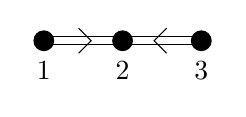
\begin{tikzpicture}[scale=0.5]
\draw (0, 0.1 cm) -- +(2 cm,0);
\draw (0, -0.1 cm) -- +(2 cm,0);
\draw[shift={(1.2, 0)}, rotate=0] (135 : 0.45cm) -- (0,0) -- (-135 : 0.45cm);
{
\pgftransformxshift{2 cm}
\draw (0 cm,0) -- (0 cm,0);
\draw (0 cm, 0.1 cm) -- +(2 cm,0);
\draw (0 cm, -0.1 cm) -- +(2 cm,0);
\draw[shift={(0.8, 0)}, rotate=180] (135 : 0.45cm) -- (0,0) -- (-135 : 0.45cm);
\draw[fill=black] (0 cm, 0 cm) circle (.25cm) node[below=4pt]{$2$};
\draw[fill=black] (2 cm, 0 cm) circle (.25cm) node[below=4pt]{$3$};
}
\draw[fill=black] (0 cm, 0 cm) circle (.25cm) node[below=4pt]{$1$};
\end{tikzpicture}
\]
If we mutate at indices 1, 3, and 2 in order we obtain the regular cluster variable
\[
x_2''' = \frac{x_1 x_2^2 z_1 z_2 z_3 z_{\ol{1}} z_{\ol{2}} z_{\ol{3}} + x_1 z_1 z_2 z_{\ol{1}} z_{\ol{2}} + x_2^2 x_3 +  x_3 z_1 z_{\ol{1}}}{x_1 x_2 x_3}
\]
with $\bfg$-vector is $\omega_2 - \omega_1$. 

Let us evaluate the level zero minor $\Delta_{\omega_2 - \omega_1}$ on a generic element
\[
g = x_{\ol{1}}(t_{\ol{1}})x_{\ol{2}}(t_{\ol{2}})x_{\ol{3}}(t_{\ol{3}})hx_3(t_3)x_2(t_2)x_1(t_1) \in \widetilde{LSp}_4^{c,c^{-1}}.
\]
To do this, fix a vector $v$ of weight $\omega_2 - \omega_1$  in $V(\omega_2 - \omega_1) \cong \kk^4[z^{\pm 1}]$. Note that $v$ is extremal in the sense that it is a highest- or lowest- weight vector for each (not necessarily simple) coroot subgroup of $\widetilde{LSP}_4$; the same property then holds automatically for any weight vector whose weight is a conjugate of $\omega_2 - \omega_1$. 

Write $e_i$ and $f_i$ for the standard generators of $\widetilde{L\mathfrak{sp}}_4$. Since $v$ sits in an $\alpha_1$-root string of length 2, we have
\[
x_1(t_1)v = v + t_1e_1v. 
\]
Similarly, since $e_1v$ has weight $s_1(\omega_2 - \omega_1) = \omega_1 - \omega_2$\sayDR{Is the equivalent weight of $\alpha_1$ given by the rows of $A$ or the columns of $A$?}, it sits in an $\alpha_2$-root string of length 2, and we have
\[
x_2(t_2)x_1(t_1)v = v + t_1e_1v + t_1t_2e_2e_1v. 
\]
Finally, $e_2e_1v$ has weight $s_2s_1(\omega_2 - \omega_1) = \omega_2 - \omega_3$, and we have
\[
x_3(t_3)x_2(t_2)x_1(t_1)v = v + t_1e_1v + t_1t_2e_2e_1v + t_1t_2t_3e_3e_2e_1v.
\]

Since we know the weights of each component of $x_3(t_3)x_2(t_2)x_1(t_1)v$, we can now compute that
\[
hx_3(t_3)x_2(t_2)x_1(t_1)v = h^{\omega_2-\omega_1}v + h^{\omega_1 - \omega_2}t_1e_1v + h^{\omega_2-\omega_3}t_1t_2e_2e_1v + h^{\omega_3-\omega_2}t_1t_2t_3e_3e_2e_1v.
\]
From here we can see that the component of $gv$ of weight $\omega_2 - \omega_1$ is
\[
(h^{\omega_2-\omega_1} + h^{\omega_1 - \omega_2}t_1t_{\ol{1}}e_1 + h^{\omega_2-\omega_3}t_1t_{\ol{1}}t_2t_{\ol{2}}e_2e_1 + h^{\omega_3-\omega_2}t_1t_{\ol{1}}t_2t_{\ol{2}}t_3t_{\ol{3}}e_3e_2e_1)v,
\]
and $\Delta_{\omega_2-\omega_1}$ is equal to the scalar by which $v$ has been multiplied in this equation. 
But now using Equation \ref{eq:frozen_values} we can check that $\Delta_{\omega_2-\omega_1}$ is equal to the formula for $x_2'''$ evaluated on $g$.
\end{proof}

\subsection{The Homogeneous Element}%\sayHW{In the process of trying to flesh out this section more, I'm a bit ambivalent about some of the notation I introduced, e.g. using $\lambda$ as a parameter for the tubes when we often use it as a weight.}\sayDR{I changed it to $\eta$ and made sure we never use this as a weight}
We conclude with an extension of Theorem~\ref{th:cluster character equals minor} motivated by the theory of canonical bases. Cluster monomials form a partial basis of a cluster algebra, and there are various meaningful (and in general different) ways of completing them to a full basis [references]. One approach in line with the considerations of this paper is to form a basis consisting of cluster characters of potentially non-rigid representations. By taking the cluster character of a generic representation with each possible $\bfg$-vector, one obtains the generic basis of \cite{Dup12} (which directly generalizes the dual semicanonical basis of Lusztig).

When $Q$ is an acyclic orientation of an $n$-cycle as in Section~\ref{sec:rigidregular}, the simplest example of a non-rigid representation is the representation $\Qrep_\eta$ at the base of a homogeneous tube $\mathcal{T}_\eta$, $\eta \in \kk^*$. That is, $\Qrep_\eta$ consists of a one-dimensional vector space at each vertex of $Q$, with arrows acting by isomorphisms such that the monodromy around $Q$ is equal to $\eta$. The dimension vector of $\Qrep_\eta$ is the minimal imaginary root $\delta$, and if $i_1<\cdots<i_m$ and $o_1<\cdots < o_m$ denote the sinks and sources of $Q$, its $\bfg$-vector is 
\[
\bfg(\Qrep_\eta) = \sum_{j=1}^m \omega_{o_j} - \omega_{i_j}.
\]
The cluster character of $\Qrep_\eta$ is independent of $\eta$, and we refer to the resulting element of the generic basis as the homogeneous element.

%We conclude with a final suggestive result which is proven exactly as Theorem~\ref{th:cluster character equals minor}.
\begin{theorem}\label{thm:homogeneous}
In $\cA_{\Qdp} \cong \kk[\widetilde{LSL}_n^{c,c^{-1}}]$ the homogeneous element $x_{\Qrep_\eta}$ is the restriction of the level zero minor $\Delta_{\bfg(\Qrep_\eta)}$. 
%  Let $D$ be any indecomposable representation $Q$ with dimension vector $\delta=\sum\limits_{i\in Q_0}\alpha_i$ and all maps isomorphisms.  Under the identification $\kk[G^{c,c^{-1}}] \cong A_Q$ we have
%  \[x_D = \Delta_{\omega_S}\]
%  for $S=[i_1,o_1-1] \cup [i_2,o_2-1] \cup \cdots \cup [i_m,o_m-1]$, where $i_1<o_1<\cdots<i_m<o_m<i_1$ denote the sinks and sources of $Q$ in the cyclic ordering of vertices.
\end{theorem}
\begin{proof}
Similar to Lemma~\ref{lem:regulargvectors}, we have $\bfg(M_\eta) = \omega_S$, where
\[
S=[i_1,o_1-1] \cup [i_2,o_2-1] \cup \cdots \cup [i_m,o_m-1] \subset \ZZ_n.
\]
The proof now proceeds exactly like that of Theorem~\ref{th:cluster character equals minor}, and we omit the details. 
%$S=[i_1,o_1-1] \cup [i_2,o_2-1] \cup \cdots \cup [i_m,o_m-1]$, where $i_1<o_1<\cdots<i_m<o_m<i_1$
\end{proof}

%While the element $x_D$ is not a cluster variable of $\cA_Q$, it is contained in the generic basis \cite{Dup12}.  It would be interesting to study the relationship of minors whose weights are $g$-vectors of other representations in the tubes with the generic basis elements.

%This suggests the study of minors whose weights are $g$-vectors of other representations in the tubes.  It turns out that these other minors do not belong to the generic basis as they do not satisfy the relations of \cite[Lemma 5.2]{Dup12}.

\begin{remark}
Theorem~\ref{thm:homogeneous} has an analogue for an arbitrary symmetric Kac-Moody group of rank two, at least formally. Let $Q$ be the $n$-Kronecker quiver: it has two vertices, and $n$ arrows from vertex 2 to vertex 1. Note that all non-initial cluster variables of $\cA_Q$ are either preprojective or postinjective. However, it contains a homogeneous element $x_M$, where $M$ is any representation with $M_1$ and $M_2$ one-dimensional and at least one arrow acting by an isomorphism. Using the obvious injective resolution of $M$ and the fact that its only nontrivial proper submodule is $S_1$, we have
\[
x_M = x_1^{-1}x_2^{n-1}(1 + \hat{y}_1 + \hat{y}_1 \hat{y}_2).
\]

On the other hand, we have $\cA_{\Qdp} \cong \kk[G^{c,c^{-1}}]$, where $G$ is the Kac-Moody group with Cartan matrix 
\[
A = \begin{bmatrix} 2 & -n \\ -n & 2 \end{bmatrix}
\]
and $c = s_1 s_2$. Let us formally compute the minor $\Delta_{\bfg(M)}$, where $\bfg(M) = (n-1) \omega_2 - \omega_1$. That is, we suppose there exists a representation $V(\bfg(M))$ of $G$ having a one-dimensional extremal weight space of weight $\bfg(M)$ (i.e. this weight space is either highest- or lowest-weight for both simple root subgroups of $G$).
\end{remark}

\section{Conventions}

\begin{itemize}

  \item 
    The Cartan matrix is $A=(a_{ij})$ and it's $n \times n$.

  \item 
    $I=[1,n]$ is the set of indices of the nodes of the Dynkin diagram. The labels are such that $c=s_1\dots s_n$.

  \item 
    $B_c$ is the matrix given by
    \[
      b_{ij} = \begin{cases}
        -a_{ij} & i<j\\
        a_{ij}  & i>j\\
        0       & i=j
      \end{cases}
    \]
    (negative below the diagonal)

  \item
    The Euler matrix $E_c$ is given by
    \[
      e_{ij} = \begin{cases}
        0       & i<j\\
        a_{ij}  & i>j\\
        1       & i=j
      \end{cases}
    \]
    (negative below the diagonal, 0 above)

  \item
    The initial $B$-matrix for $G^{c,c^{-1}}$ with double reduced word $\bar 1,\dots,\bar n,n\dots 1$ is
    \[
      \left[
        \begin{array}{c}
          B_c\\
          E_{c^{-1}}\\
          E_{c^{-1}}
        \end{array}
      \right]
    \]
  
  \item 
    The minor $\Delta_\omega^\delta$ is our notation for YZ's $\Delta_{\delta, \omega}$.
  
  \item 
    $[\alpha:\alpha_j]$ notation defined immediately before \Cref{lem:minorsondbc}
  
  \item 
    The transpose $g \mapsto g^T$ of YZ is defined in passing without notation in the proof of \Cref{lem:minorsondbc}.
  
  \item 
    $L_{\omega_i}$ is the $i$-th fundamental representation in the proof of \Cref{lem:minorsondbc}.

  \item 
    Used the notation $h^\omega$ for $\omega$ a weight and $h \in H$ without explaining it in the proof of \Cref{lem:minorsondbc}.

  \item 
    We use $x_{-i}(t)$ rather than a barred version for negative 1-parameter subgroups in the proof of \Cref{lem:minorsondbc}.

  \item 
    The identity $\beta_j^+ + \sum_{i=1}^{j-1} a_{ij} \beta_i^+ = \alpha_j$ is used in the proof of \Cref{lem:minorsondbc} without comment.
\end{itemize}

  \begin{lemma}\sayDR{This should be translated into our current notation and placed in an appropriate location.}\sayHW{The final sentence before the main theorem in Section 4.2 I think now accomplishes ass that is needed.}
    Let $g$ be a generic element of $L^{c,c^{-1}}$.
    \begin{enumerate}
      \item $\Delta_{\omega_i}(g)=u_i^{-1}$
      \item $\Delta_{c\omega_i}^{\omega_i}(g)=\begin{cases}u_i^{-1}\prod\limits_{j=i^-}^{i^+}t_j & \text{if $i$ is a sink in $Q$;}\\u_i^{-1}t_i & \text{if $i$ is a source in $Q$;}\\u_i^{-1}\prod\limits_{j=i}^{i^+}t_j & \text{if $i$ is neither a source nor a sink in $Q$ but $i^+$ is a source;}\\u_i^{-1}\prod\limits_{j=i^-}^it_j & \text{if $i$ is neither a source nor a sink in $Q$ but $i^-$ is a source.}\end{cases}$
      \item For 
      \begin{equation}
        y_i=\begin{cases}\Delta_{c\omega_i}^{\omega_i} & \text{if $i$ is a sink in $Q$;}\\\Delta_{c\omega_i}^{\omega_i}\left(\Delta_{c\omega_{i_-}}^{\omega_{i_-}}\Delta_{c\omega_{i_+}}^{\omega_{i_+}}\right)^{-1} & \text{if $i$ is a source in $Q$;}\\\Delta_{c\omega_i}^{\omega_i}\left(\Delta_{c\omega_{i_+}}^{\omega_{i_+}}\right)^{-1} & \text{if $i$ is neither a source nor a sink in $Q$ but $i^+$ is a sink;}\\\Delta_{c\omega_i}^{\omega_i}\left(\Delta_{c\omega_{i_-}}^{\omega_{i_-}}\right)^{-1} & \text{if $i$ is neither a source nor a sink in $Q$ but $i^-$ is a sink.}\end{cases}
      \end{equation}
      we have
      \begin{align}
        y_i(g)&=\begin{cases}u_i^{-1}t_i & \text{if $i$ is a sink in $Q$;}\\u_{i_-}u_i^{-1}u_{i_+}t_i & \text{if $i$ is a source in $Q$;}\\u_i^{-1}u_{i_+}t_i & \text{if $i$ is neither a source nor a sink in $Q$ but $i^+$ is a sink;}\\u_{i_-}u_i^{-1}t_i & \text{if $i$ is neither a source nor a sink in $Q$ but $i^-$ is a sink.}\end{cases}
      \end{align}
    \end{enumerate}
  \end{lemma}



% bibliography
\bibliographystyle{amsalpha}
\bibliography{bibliography}

\end{document}

% a test for Harold
